
\documentclass[12pt,a4paper,oneside]{article}
\usepackage[margin=1.2in]{geometry}
\usepackage{appendix}
\usepackage[dvips]{graphicx}
\usepackage{epsfig}
\usepackage{amsmath}
\usepackage{amssymb}
\usepackage{psfrag}
\usepackage[square, comma,sort,numbers]{natbib}
\usepackage{fancyhdr}
\usepackage[nottoc]{tocbibind}
\usepackage{color}
\usepackage{fixltx2e}
\usepackage{pdfpages}
\usepackage{pdflscape}
\usepackage{booktabs}
\usepackage{graphicx}
\usepackage{float}
\usepackage{afterpage}
\usepackage{subcaption}
\usepackage{lscape}
\usepackage{rotating}
\usepackage{enumitem}
\usepackage{array,tabularx}
\usepackage{fancyref}
\usepackage[dvipsnames]{xcolor}
\usepackage[colorlinks=true,allcolors=blue]{hyperref}%



\newcommand{\quotes}[1]{``#1''}

\newenvironment{conditions*}
  {\par\vspace{\abovedisplayskip}\noindent
   \tabularx{\columnwidth}{>{$}l<{$} @{\ : } >{\raggedright\arraybackslash}X}}
  {\endtabularx\par\vspace{\belowdisplayskip}}



\pagestyle{fancy}
\title{\Huge The Hat Creek Radio Observatory\\
\vspace{0.5cm}
The Attemplifier Module\\
\vspace{0.5cm}
\normalsize \emph{}
\vspace{3.5cm}
\begin{center}

\includegraphics[height=4cm]{titlepage/SETI_institute_logo.jpg}
\end{center}
}
\author{ 
\vspace{1cm}
\Large
\textbf{ Alexander Pollak \& Sarah Schoultz} \\
SETI Institute \\ 
189 Bernardo Ave, Suite 200 \\
Mountain View, CA 94043 \\ 
Alexander.Pollak.87@gmail.com\\
}
\date{\today}



\begin{document}
\clearpage\maketitle
\thispagestyle{empty}

%\newpage
%\thispagestyle{empty}
%\section*{Abstract}
%\noindent 
%



%
%\vspace{3cm}
%\begin{flushright}
%Alexander Pollak \\ \emph{September, 2015}
%\end{flushright}

%\newpage
%\thispagestyle{empty}
%\tableofcontents
\newpage

%----------------------------------------------------------------------------------------
%	General
%----------------------------------------------------------------------------------------
%\pagestyle{plain}
\section{General}
\label{sec:1}
% ----------------------------------------------------------------

This document outlines general information regarding the Attemplifier Module such as the design, parts, wiring, cabling, and testing. This information is aimed at detailing the entire process of creating an Attemplifier Module from design to manufacturing to testing. 

The attmplifiers in the module condition the power level going into the analog to digital converter (an RFSoC) to the correct value. The module itself is needed to contain and operate sixteen attemplifiers as the digitizer, an HTG-ZRF16 board by High Tech Global, being used has sixteen channels. 

Finally, please note that \emph{this module can only be operated at 110V AC.} 

%----------------------------------------------------------------------------------------
%	CAD Design and Drawings
%--------------------------------------------------------------------------------------

\section{CAD Design and Drawings}
\label{sec:2}
% ----------------------------------------------------------------
This section includes a description of the CAD design. An image of the CAD model is shown in Figure 1. One can see the internal arrangement of the control board (left rear), general power supply (front right), the Raspberry Pi power supply (middle right) the Raspberry Pi (middle rear), the two layered racks of attemplifiers (middle), and directional fan (left rear). Note that the Raspberry Pi power supply, metal case perforated with circles, is not visible in Figure \ref{fig:CAD-Iso} but is in Figure \ref{fig:CAD-above}. The lid of the enclosure, not shown in Figure \ref{fig:CAD-Iso} or \ref{fig:CAD-above}, is perforated to further increase cooling. The panel facing the viewer in Figure \ref{fig:CAD-Iso} is considered the front panel. This is important to note for future sections. The majority of the Attemplifier Module enclosure is off the shelf (PN: 24563-174) except for a few parts: the front panel, the back panel, the base plate, and the attemplifier mounting rails. These custom parts were made by Front Panel Express, and the drawings can be found in Appendix A. 

\hfill \break

%
\begin{figure}[H]
\centering
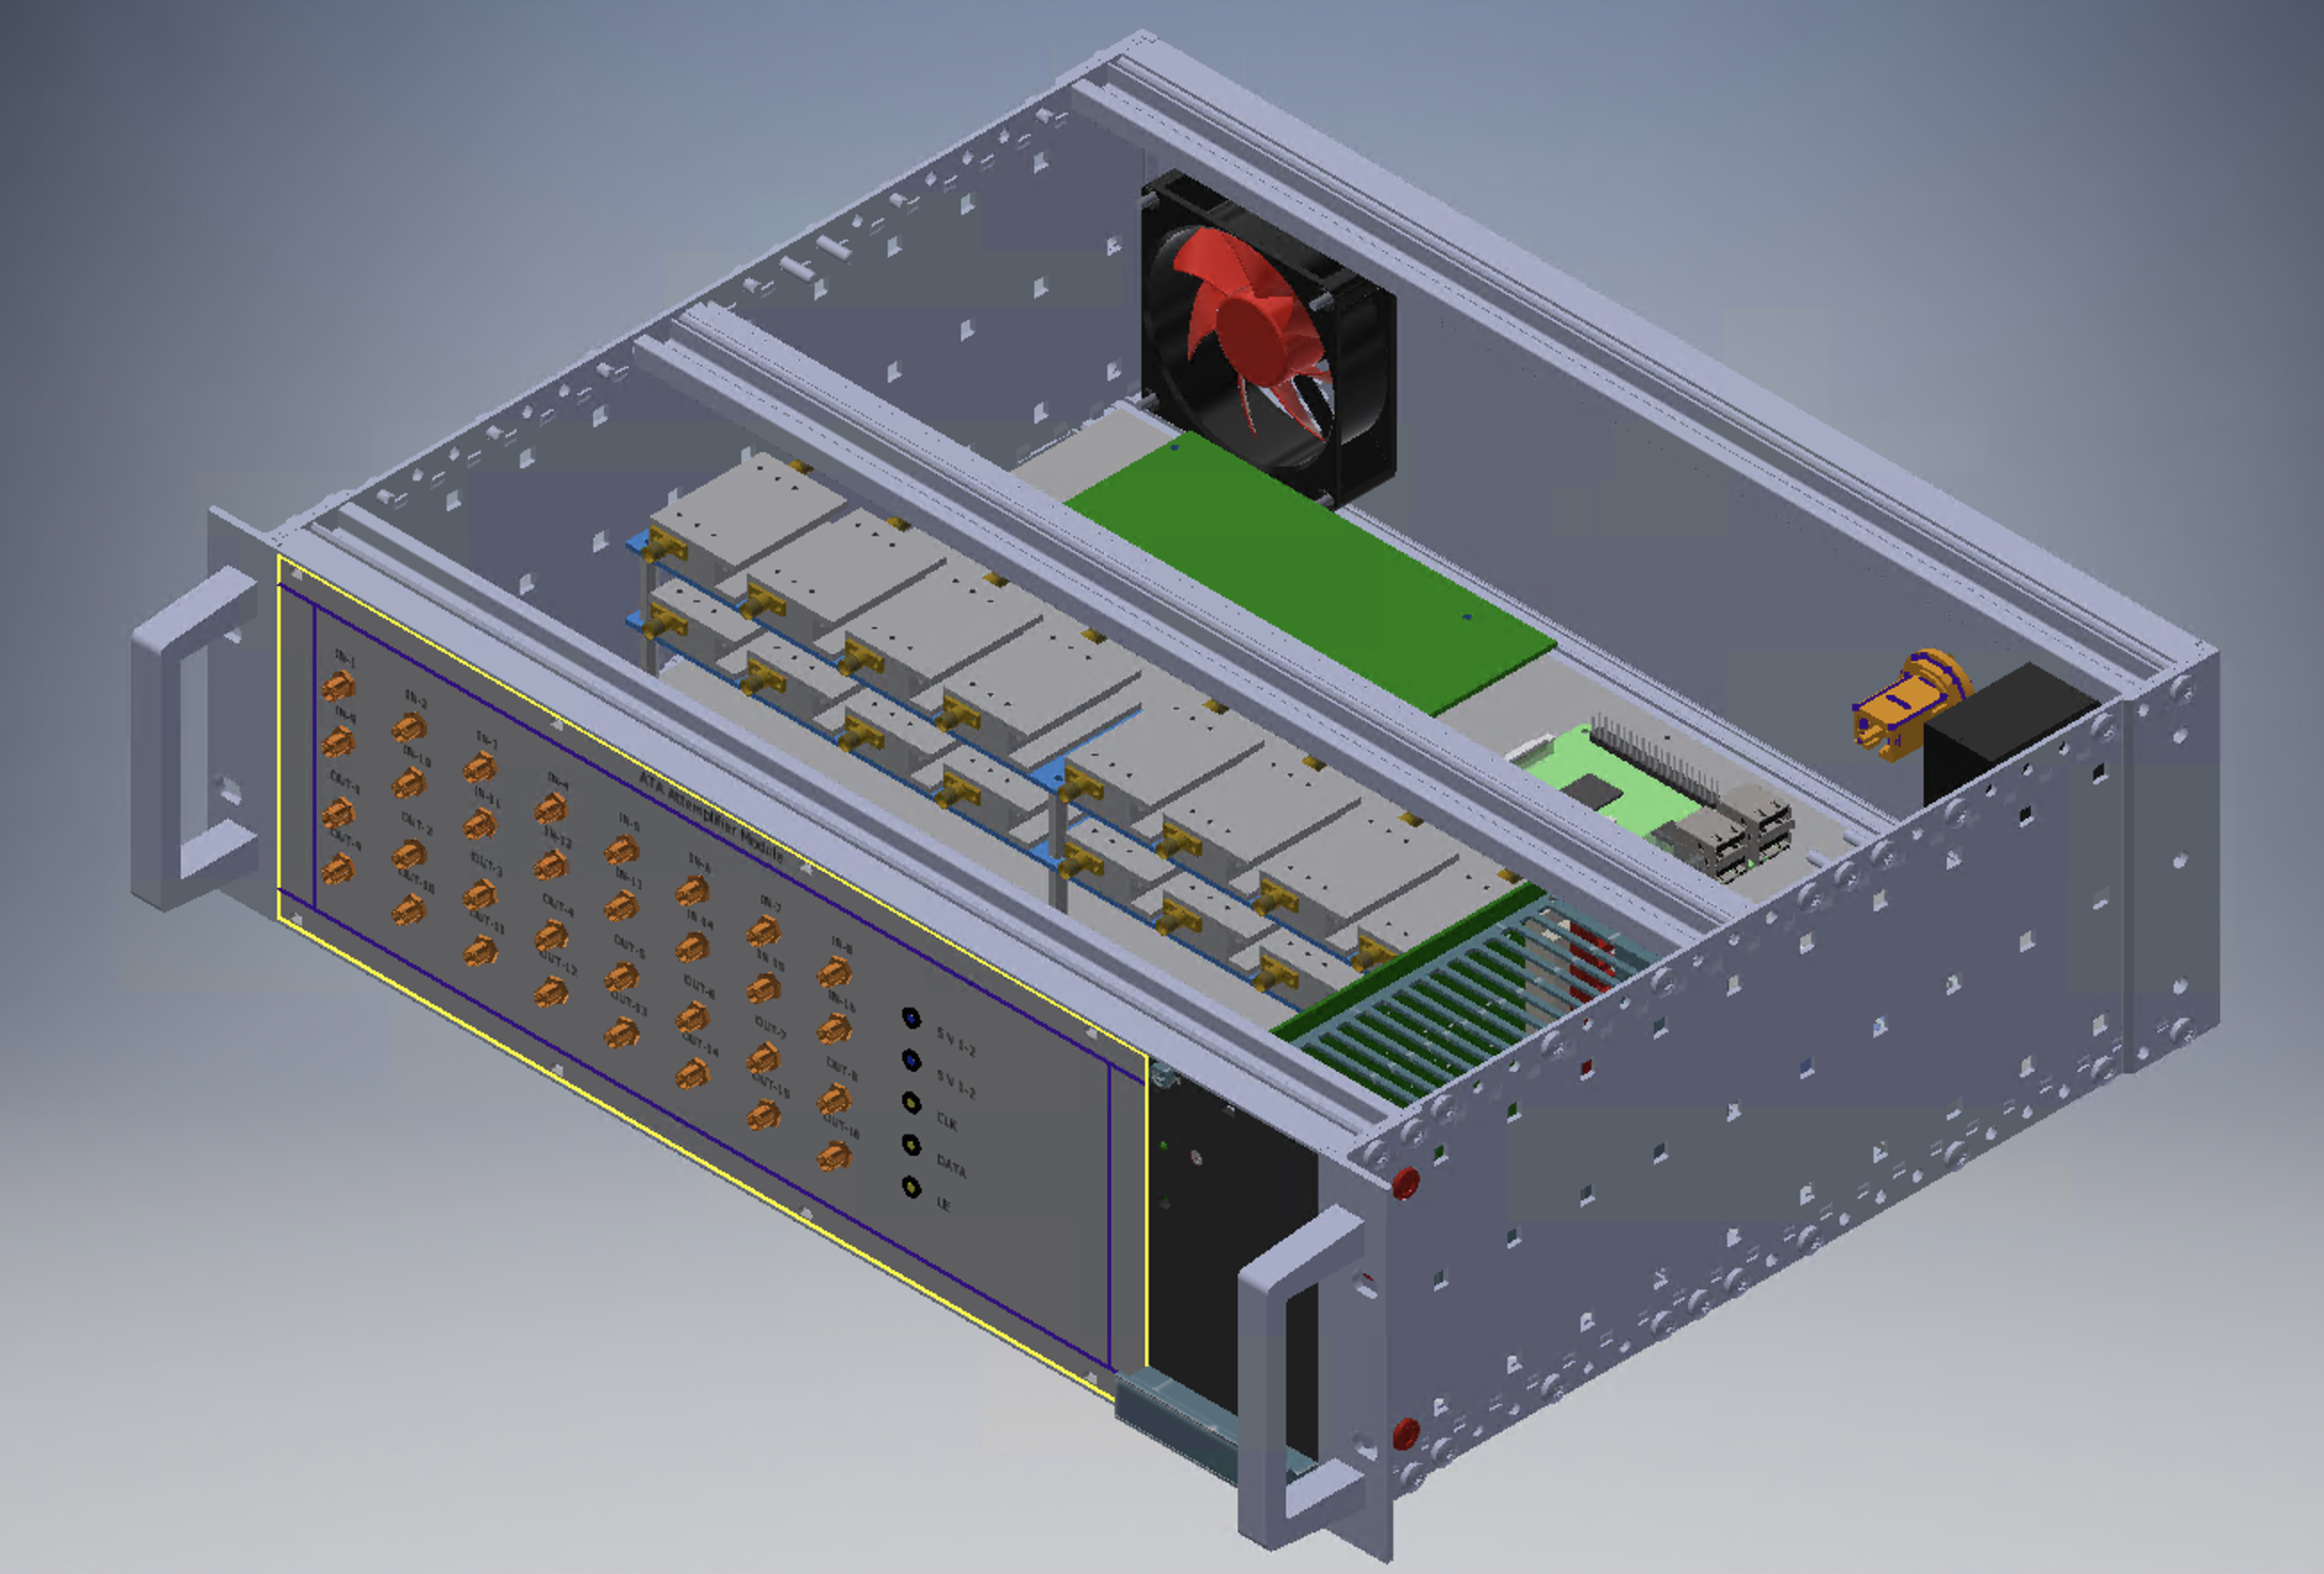
\includegraphics[width=1\linewidth]{Documentation/figures/iso view.png}
\caption{ISO view of the Attemplifier Module CAD}
\label{fig:CAD-Iso}
\end{figure}
%

%
\begin{figure}[H]
\centering
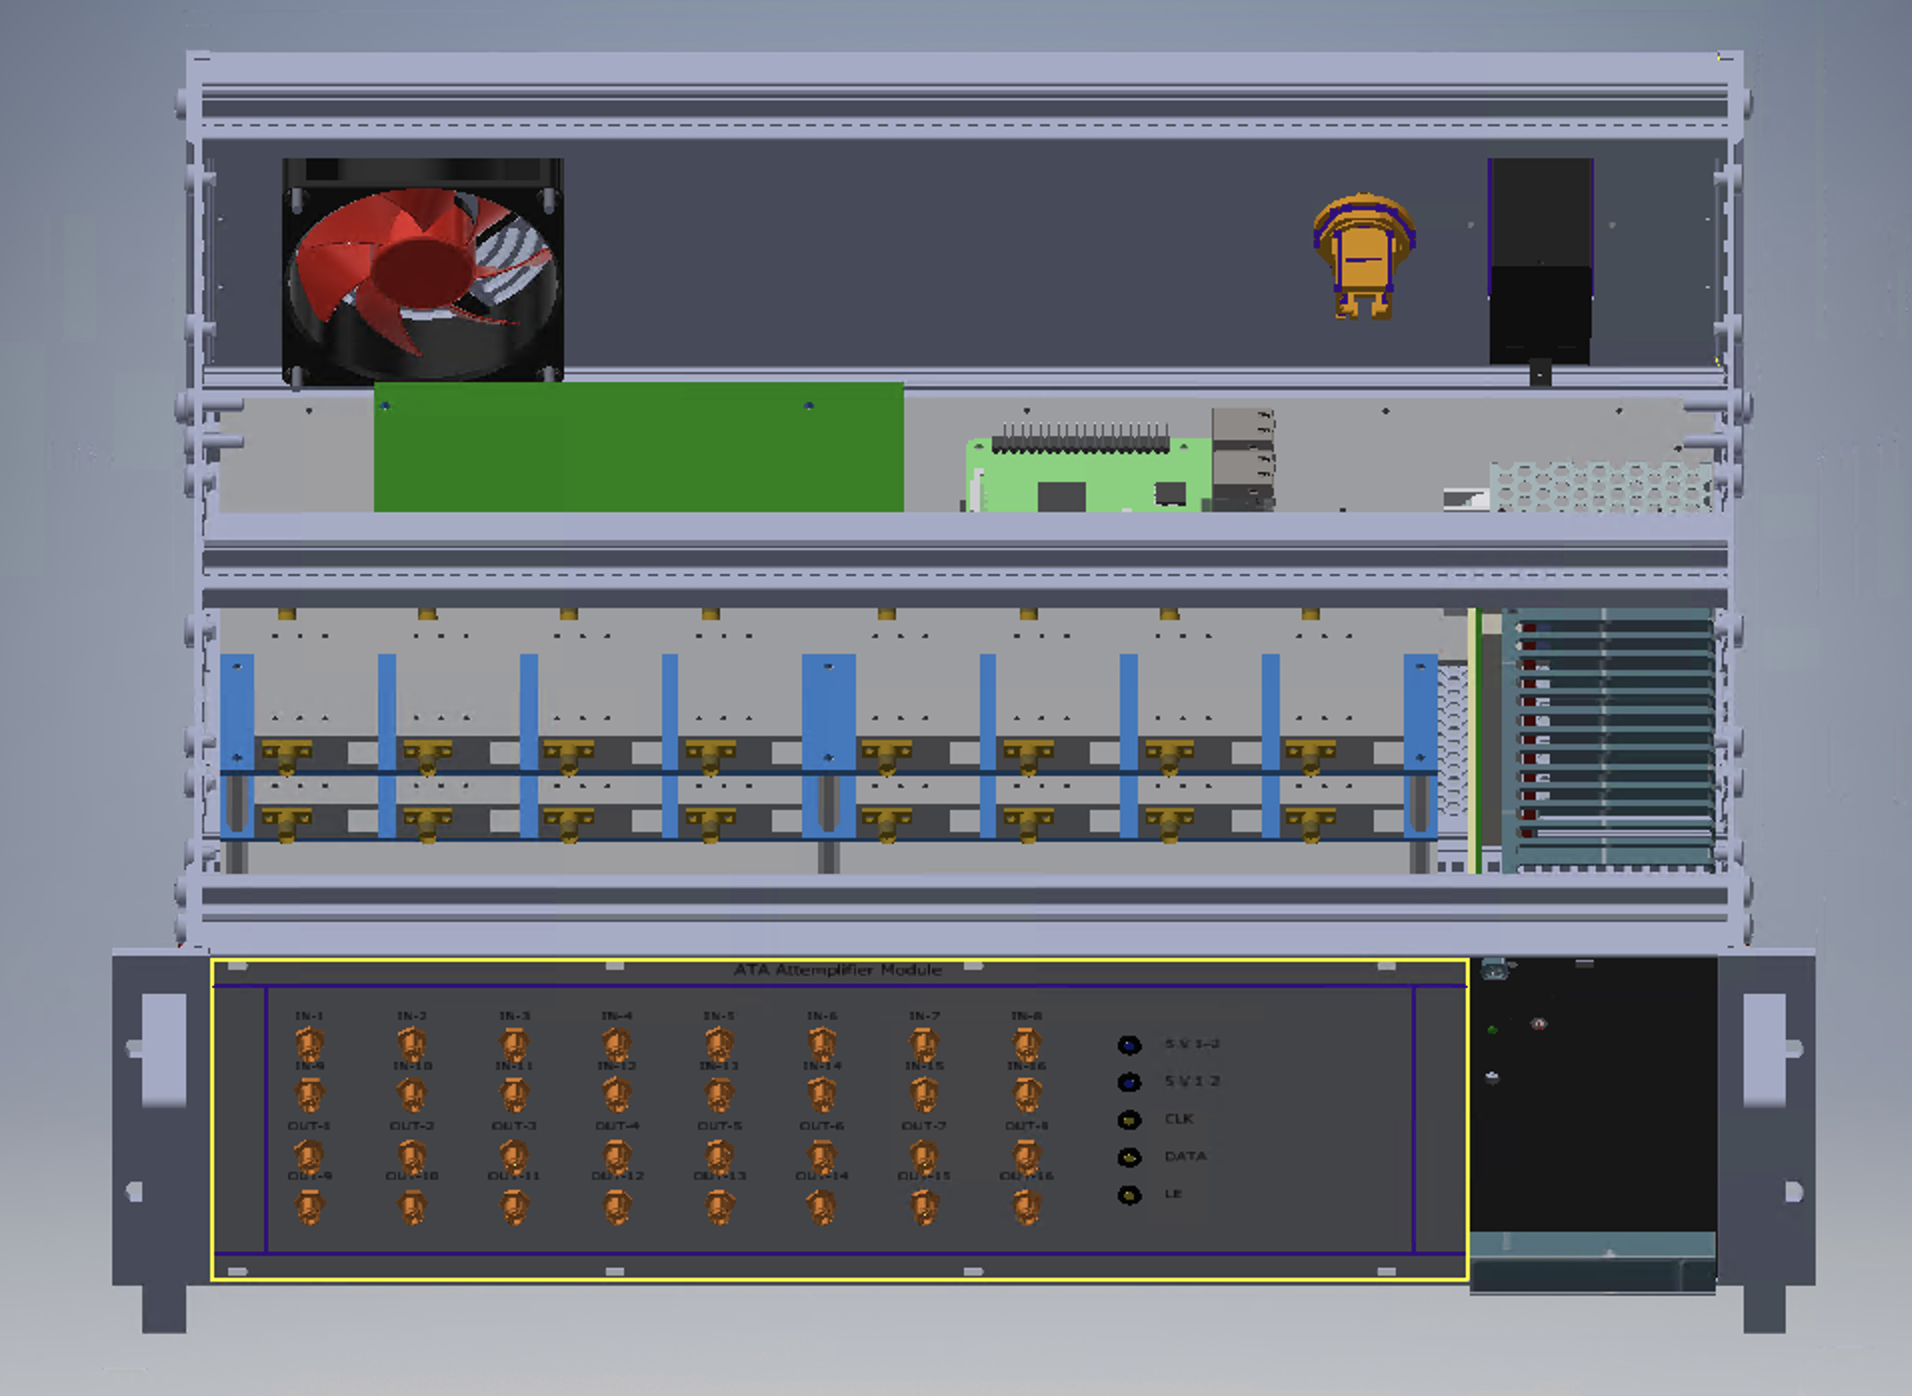
\includegraphics[width=1\linewidth]{Documentation/figures/cad_above.png}
\caption{Top View of the Attemplifier Module CAD}
\label{fig:CAD-above}
\end{figure}
%

For a part list of the Attmplifier Module, except for the attmplifiers,  control board, and some wiring parts, see Appendix B. 

%----------------------------------------------------------------------------------------
%	Control Board
%--------------------------------------------------------------------------------------

\section{Control Board}
\label{sec:3}
% ----------------------------------------------------------------

The control board is designed as an interface between the GPIOs of the Raspberry Pi and the attemplifiers. Assembled in house, see Figure \ref{fig:Control Board} for how a completed control board should look. A list of all the required parts for it appears in Appendix C. 

%
\begin{figure}[H]
\centering
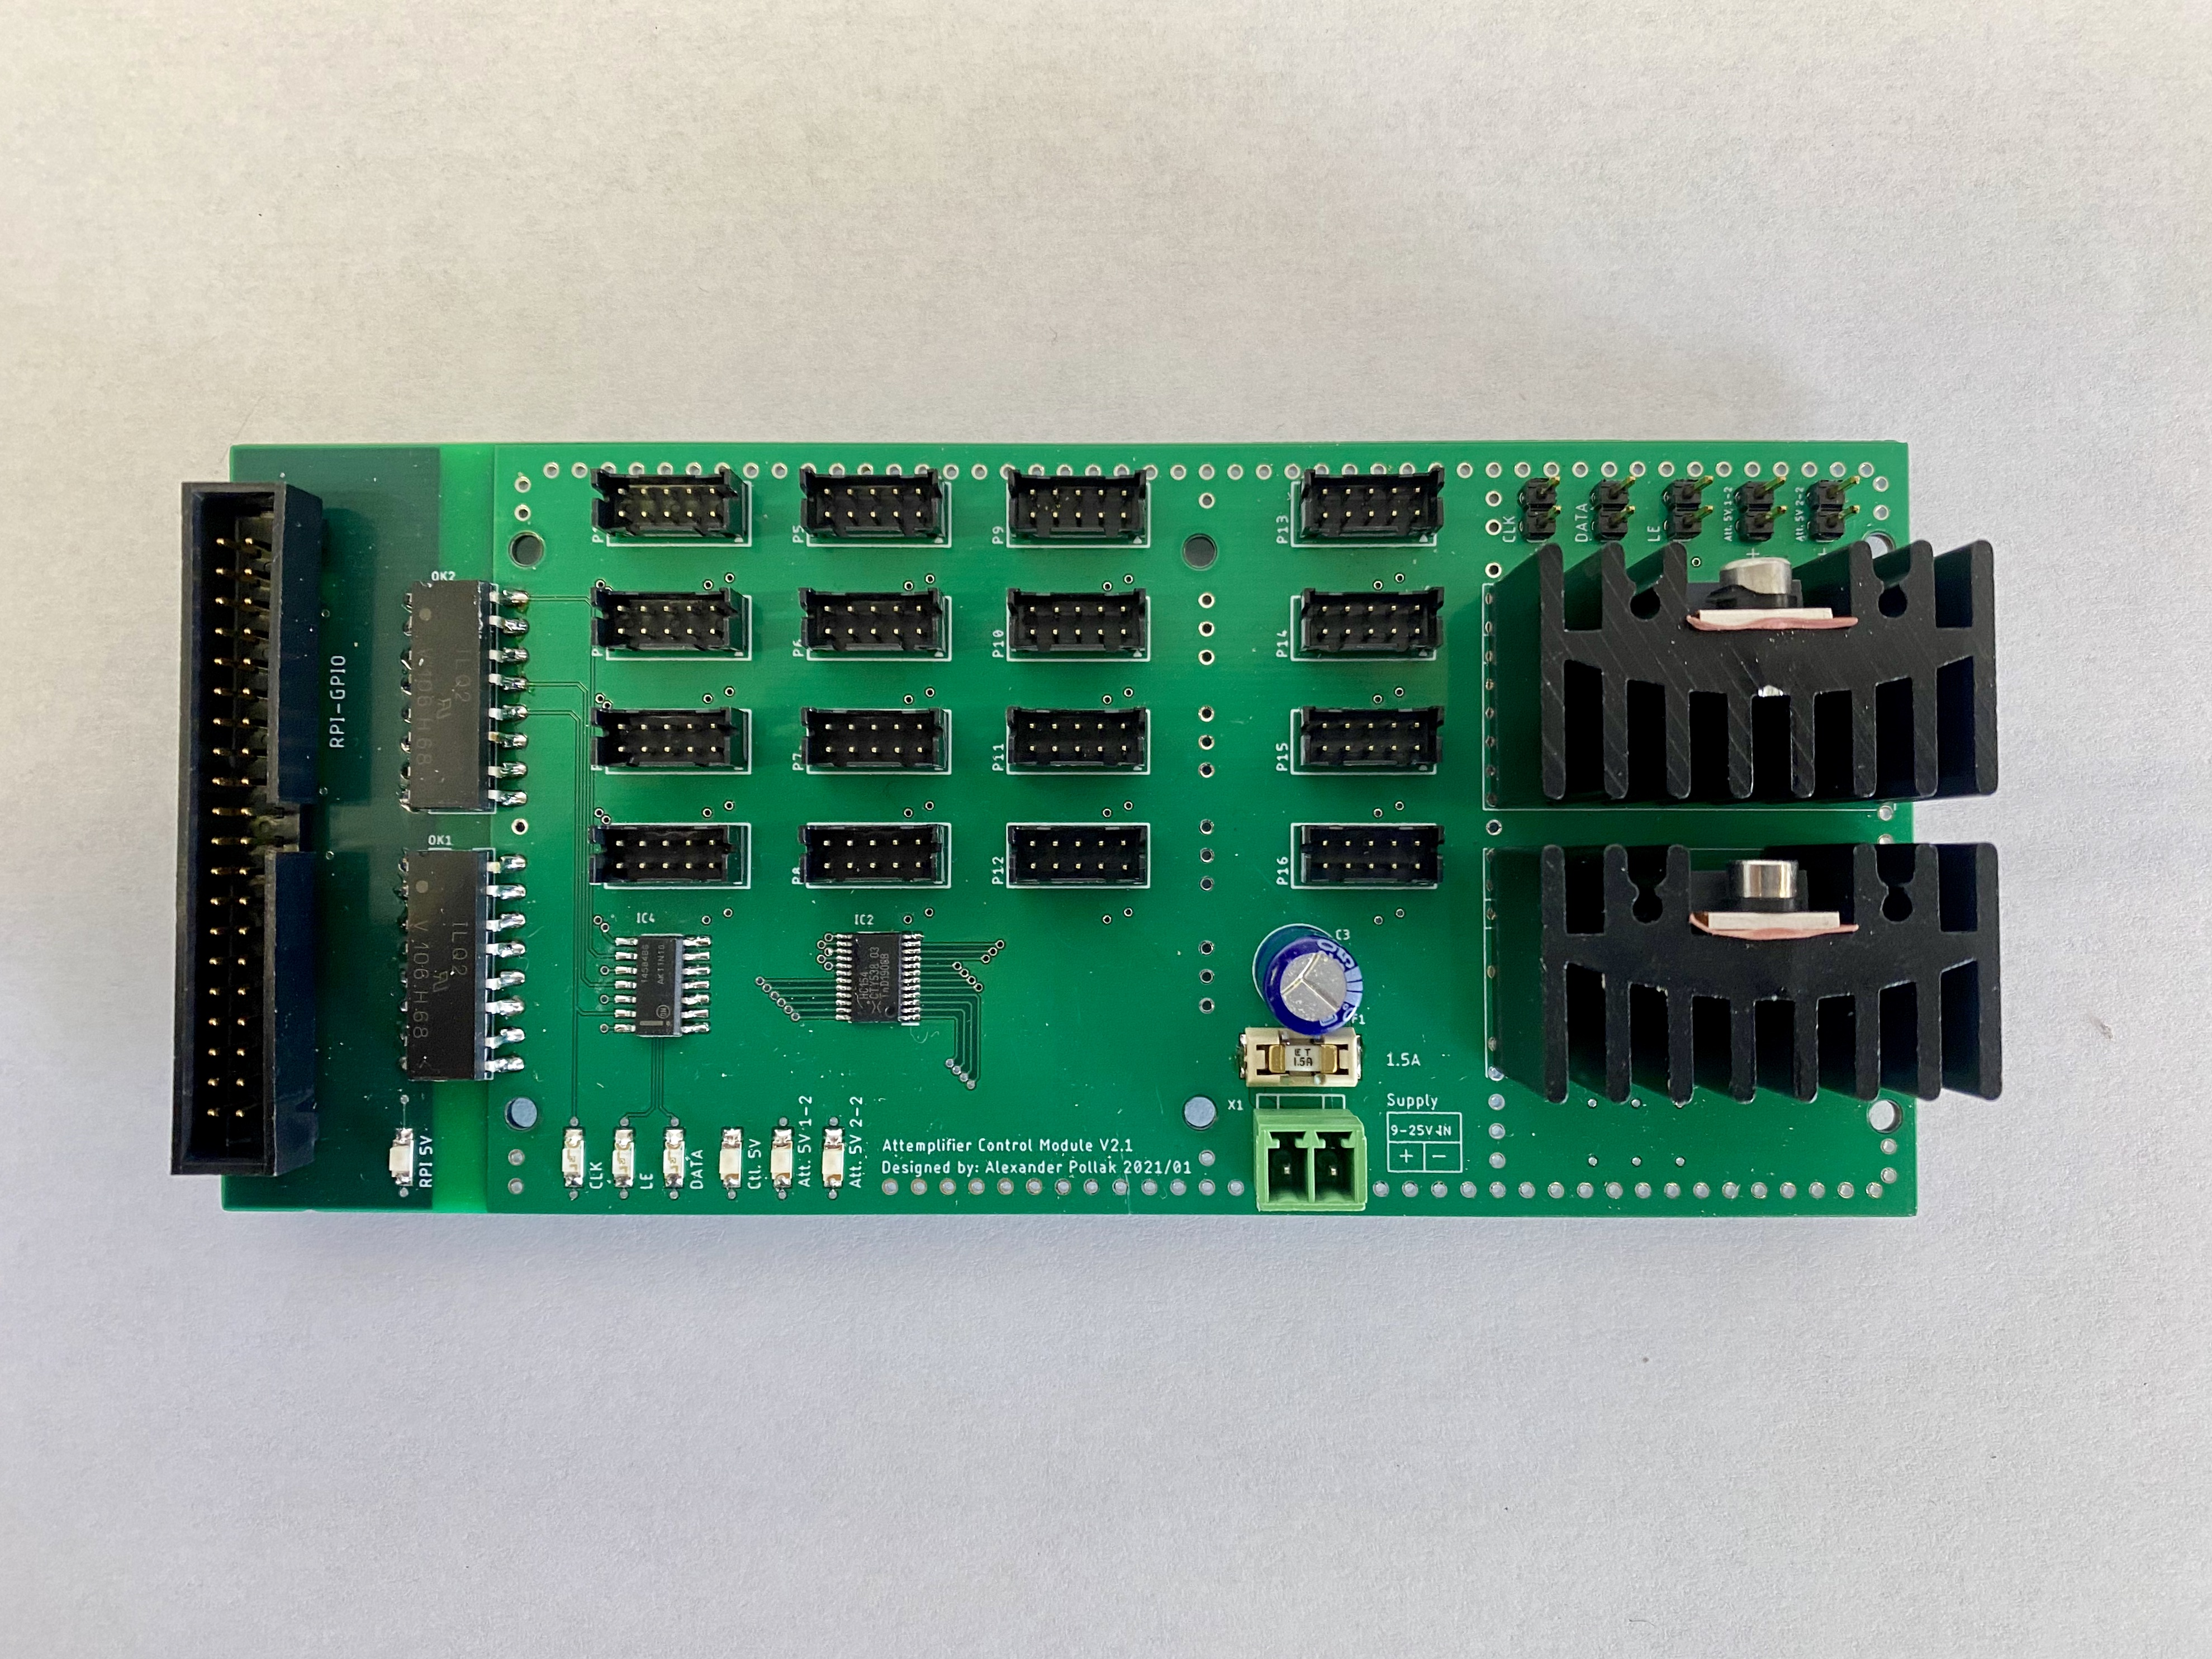
\includegraphics[width=1\linewidth]{Documentation/figures/Control Board.jpeg}
\caption{Completed Control Board}
\label{fig:Control Board}
\end{figure}
%

\subsection{Design}
\label{sec:3.1}
% ----------------------------------------------------------------

The control board electrically isolates any signals from the Raspberry Pi via optocouplers to avoid any noise contamination. The board also includes two linear voltage regulators each of which powers eight attemplifiers. The board is designed to accept 9-25V DC as an input and includes several green LEDs indicating the supply voltage of the attemplifiers and control voltage of the board. Additionally, when programming an attemplifier, the control board shows the communication signals, clock, data, latch enable, using three yellow LEDs. Both the green and yellow LEDs showing the supply voltages and communication signals are duplicated on the front panel of the module and are connected to the control board via pin-headers. All of these functionalities are reflected in the schematic, Appendix D, and layout, Figure \ref{fig:Control_Layout} of the control board. The control board voltage range is 9-25V.

%
\begin{figure}[H]
\centering
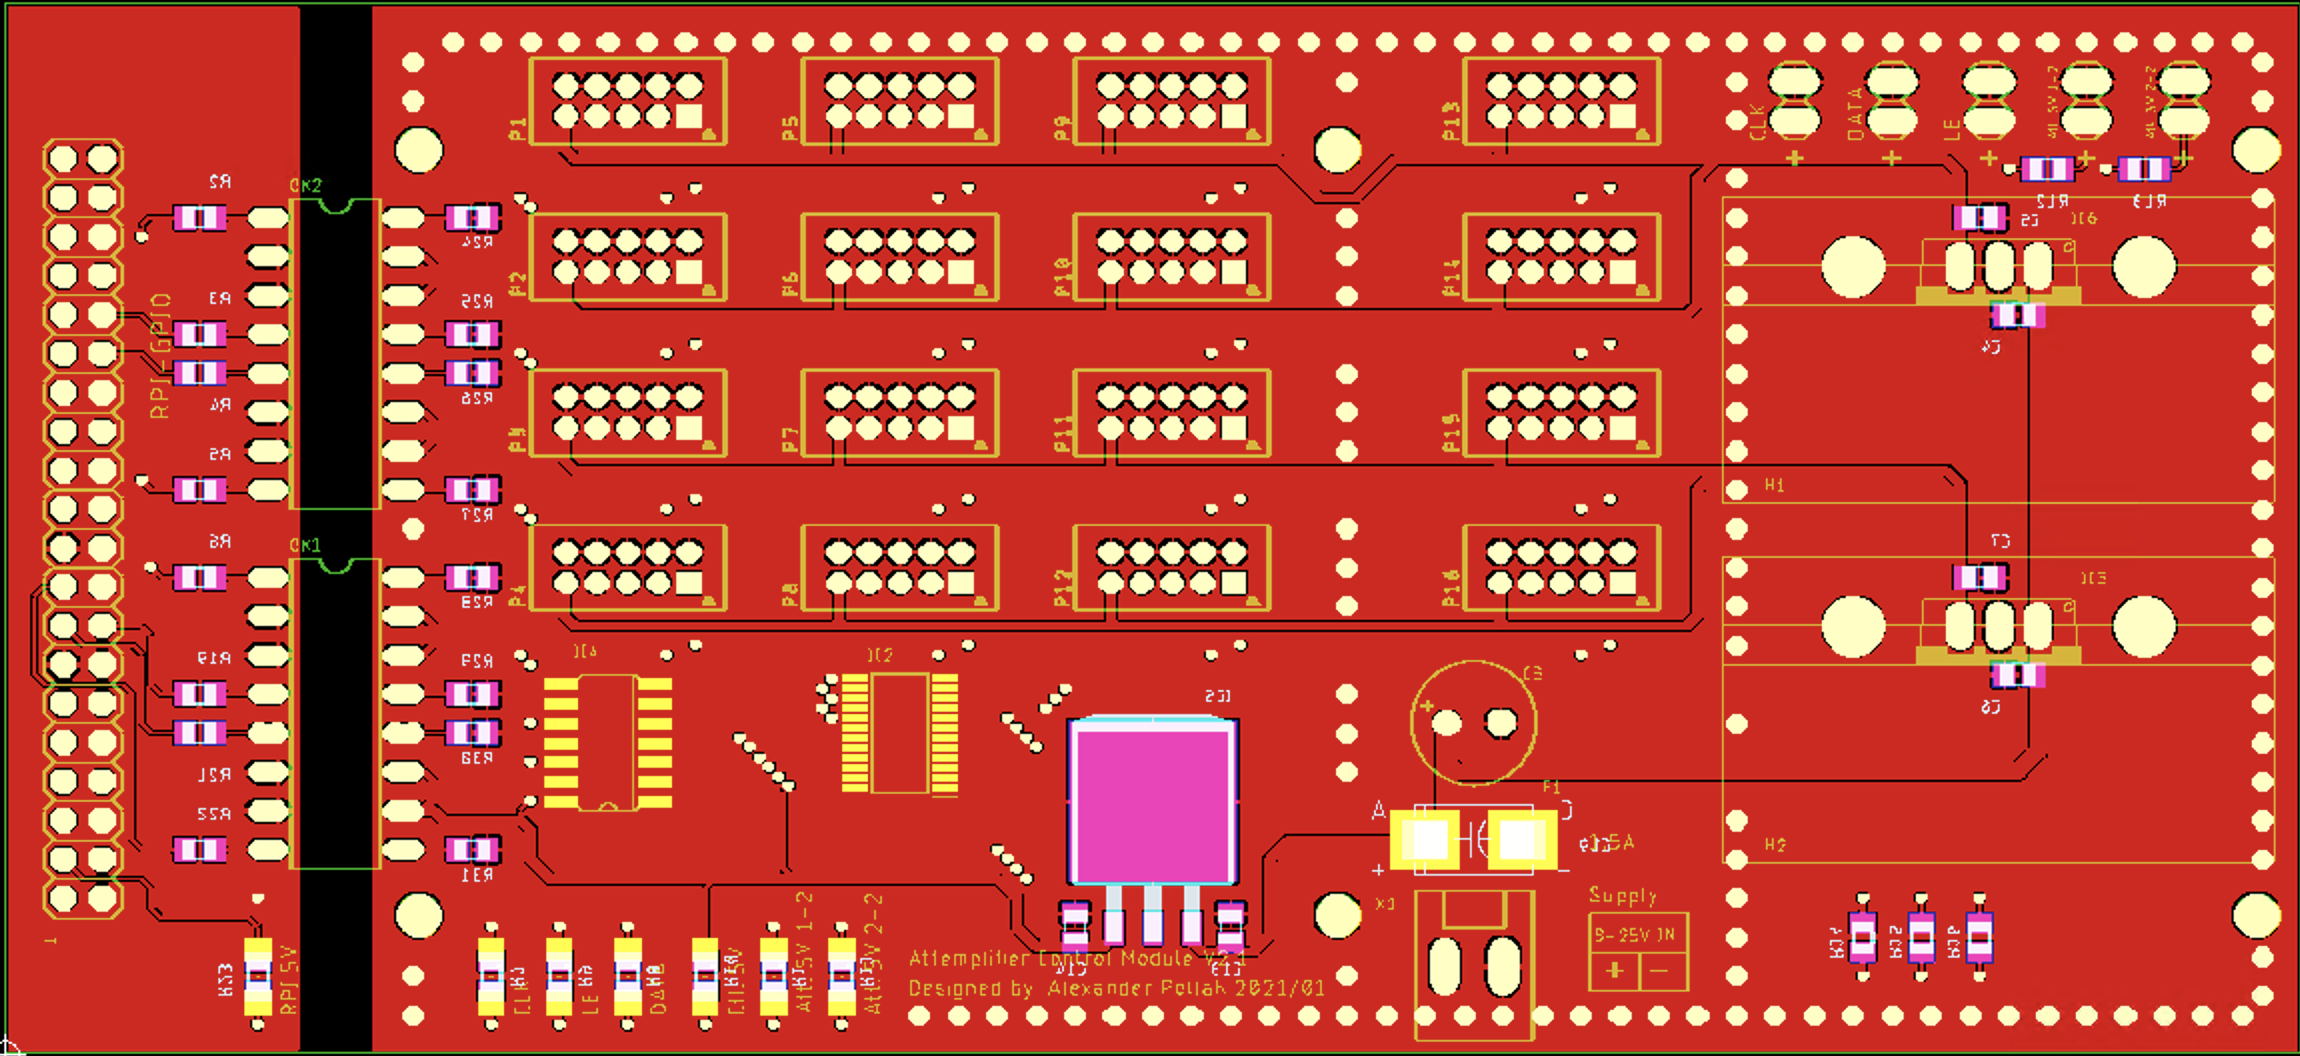
\includegraphics[width=1\linewidth]{Documentation/figures/Control_Layout.png}
\caption{Control Board Layout}
\label{fig:Control_Layout}
\end{figure}
%

%----------------------------------------------------------------------------------------
%	Attemplifiers
%--------------------------------------------------------------------------------------

\section{Attemplifiers}
\label{sec:4}
% ----------------------------------------------------------------

The purpose to the attemplifiers is to set the IF power level so that the ADCs operate with enough dynamic range and utilize the appropriate amount of bits.

\subsection{Design}
\label{sec:4.1}
% ----------------------------------------------------------------

Originally designed in 2007, the attemplifier's worked in conjunction with the IBobs. However, the IBobs have since been retired and replaced with the SNAP board and RFSOC Modules. Furthermore, 2007 attemplifier design was improved upon, and so the design that is used for the Attempifier Module is from 2012 and is called 1050-A. Figure \ref{fig:Attemp_Schem} and \ref{fig:Attemp_layout} show the electronic schematic and layout of 1050-A. For the amplifier enclosure design, go to Appendix E.

%
\begin{figure}[H]
\centering
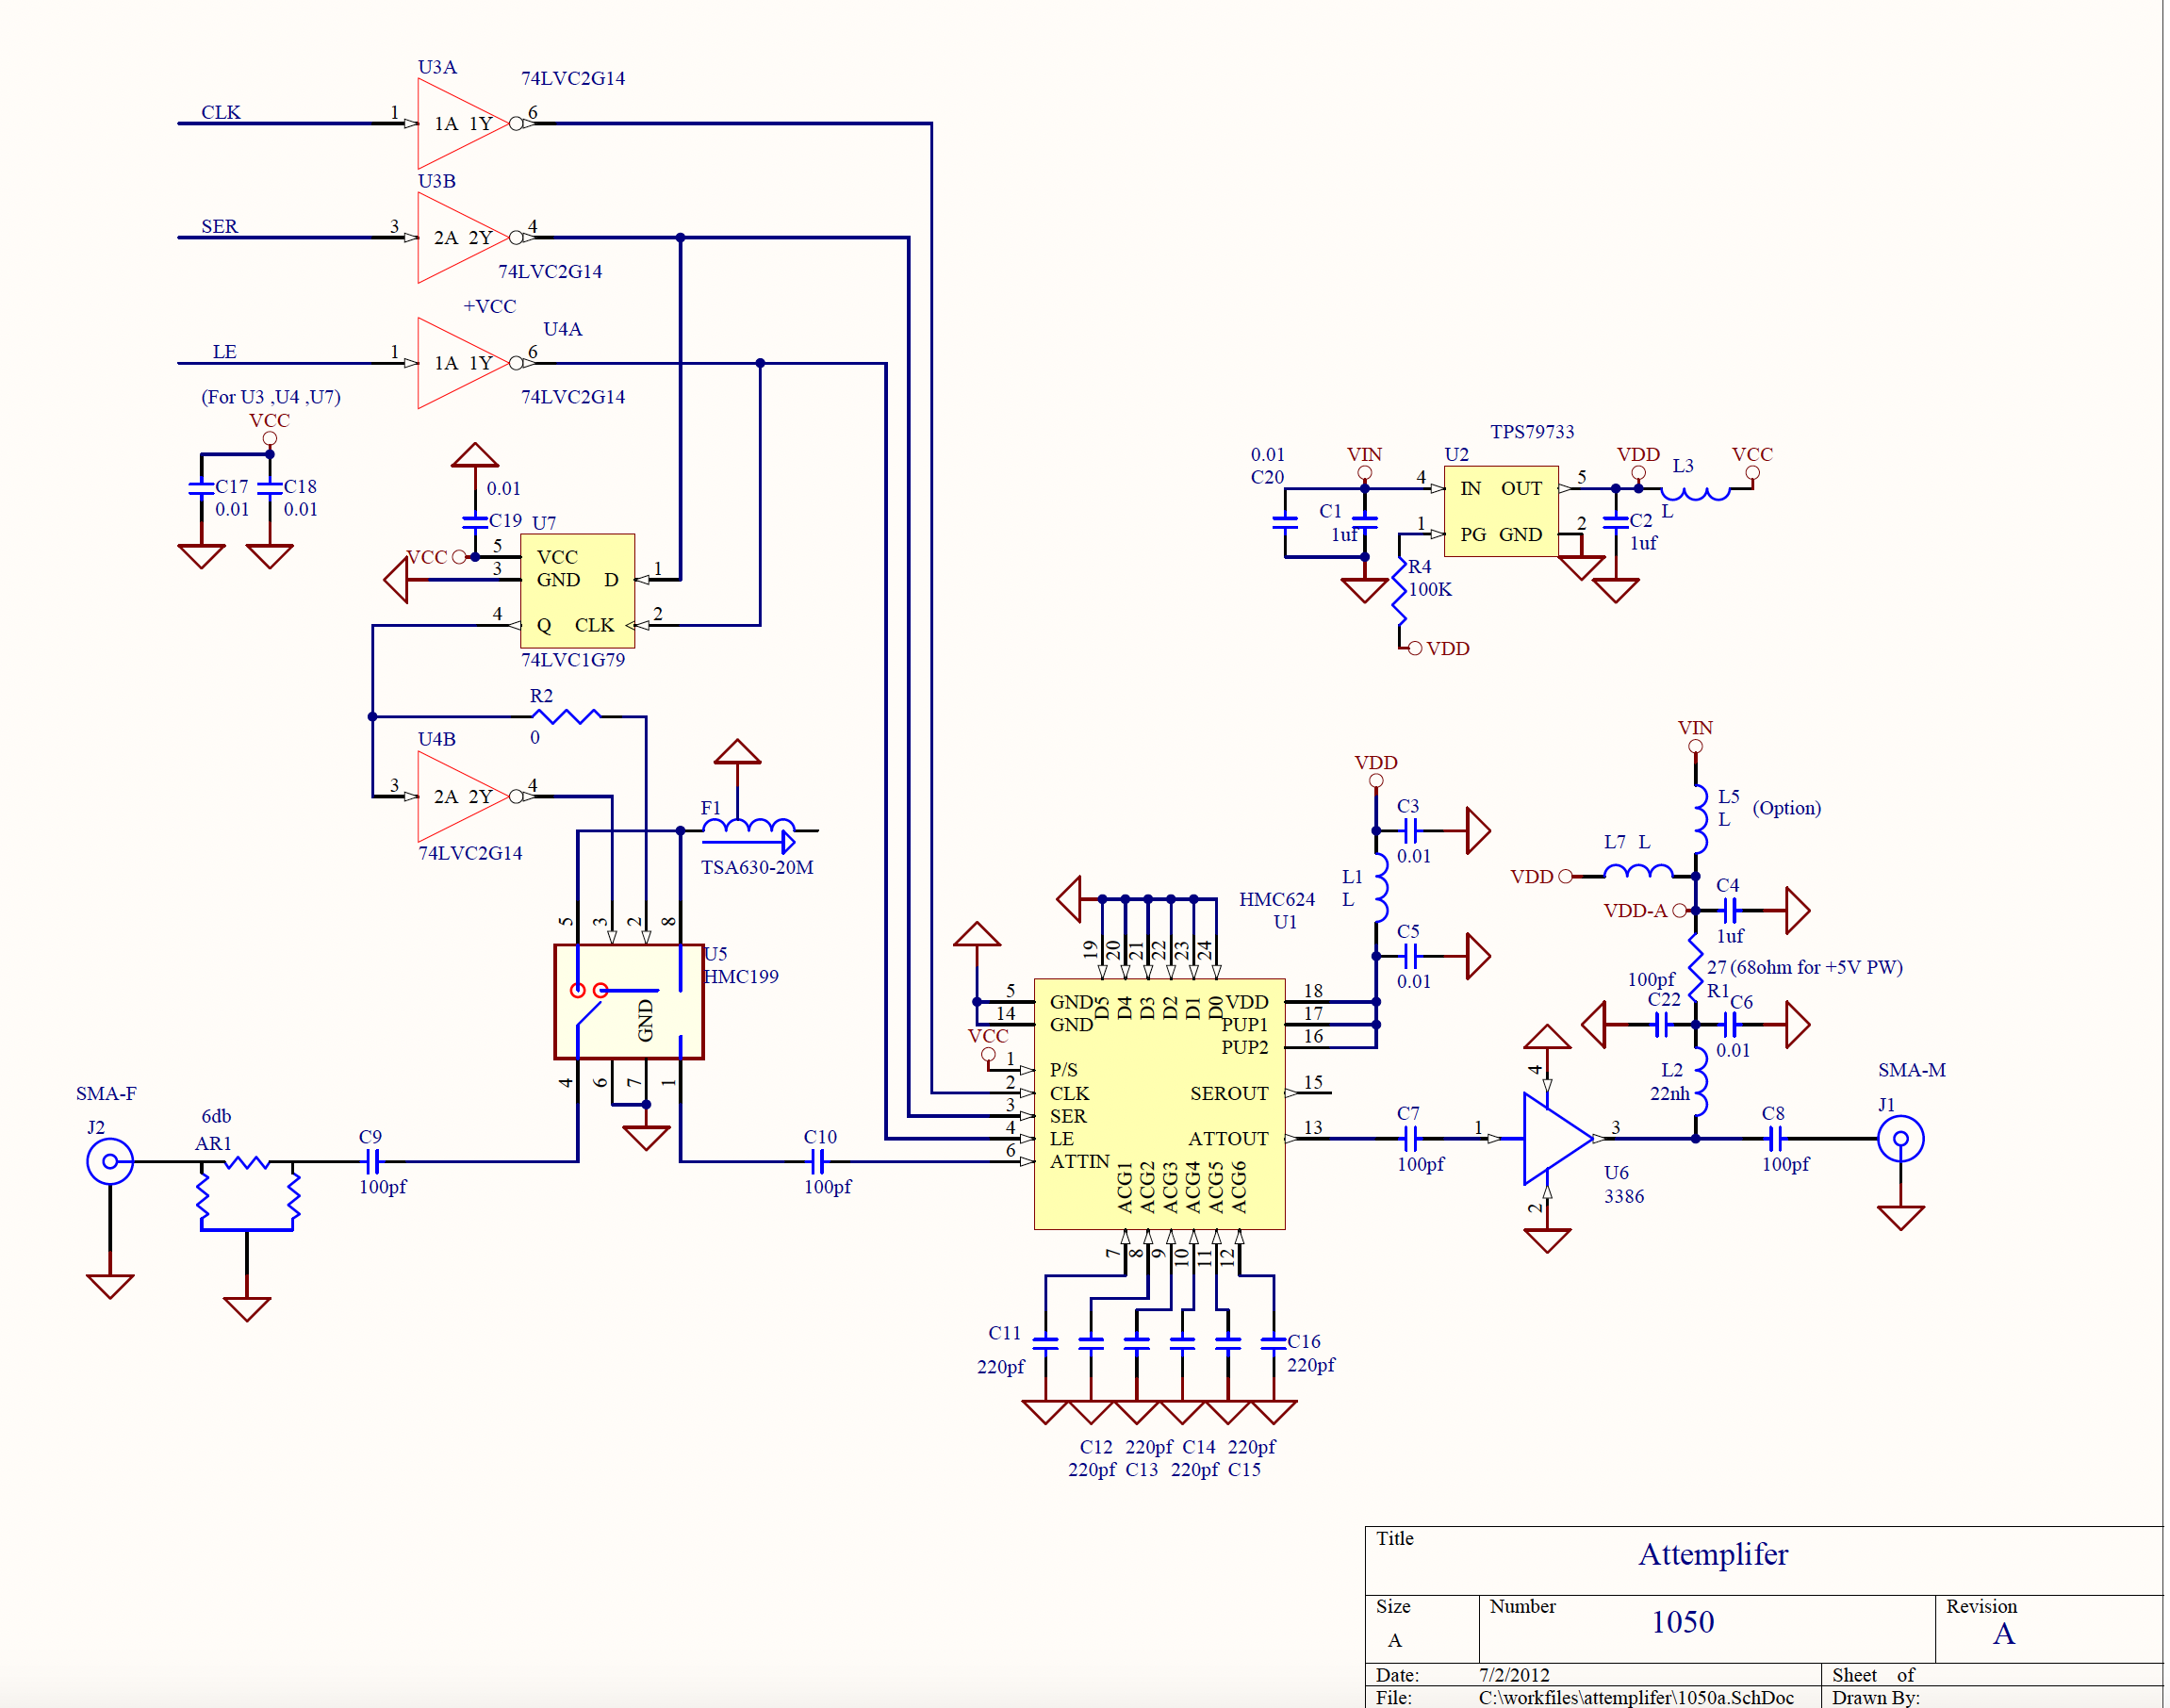
\includegraphics[width=1\linewidth]{Documentation/figures/Attemp_Schematic.png}
\caption{1050-A Attemplifier Electronics Schematic}
\label{fig:Attemp_Schem}
\end{figure}
%

%
\begin{figure}[H]
\centering
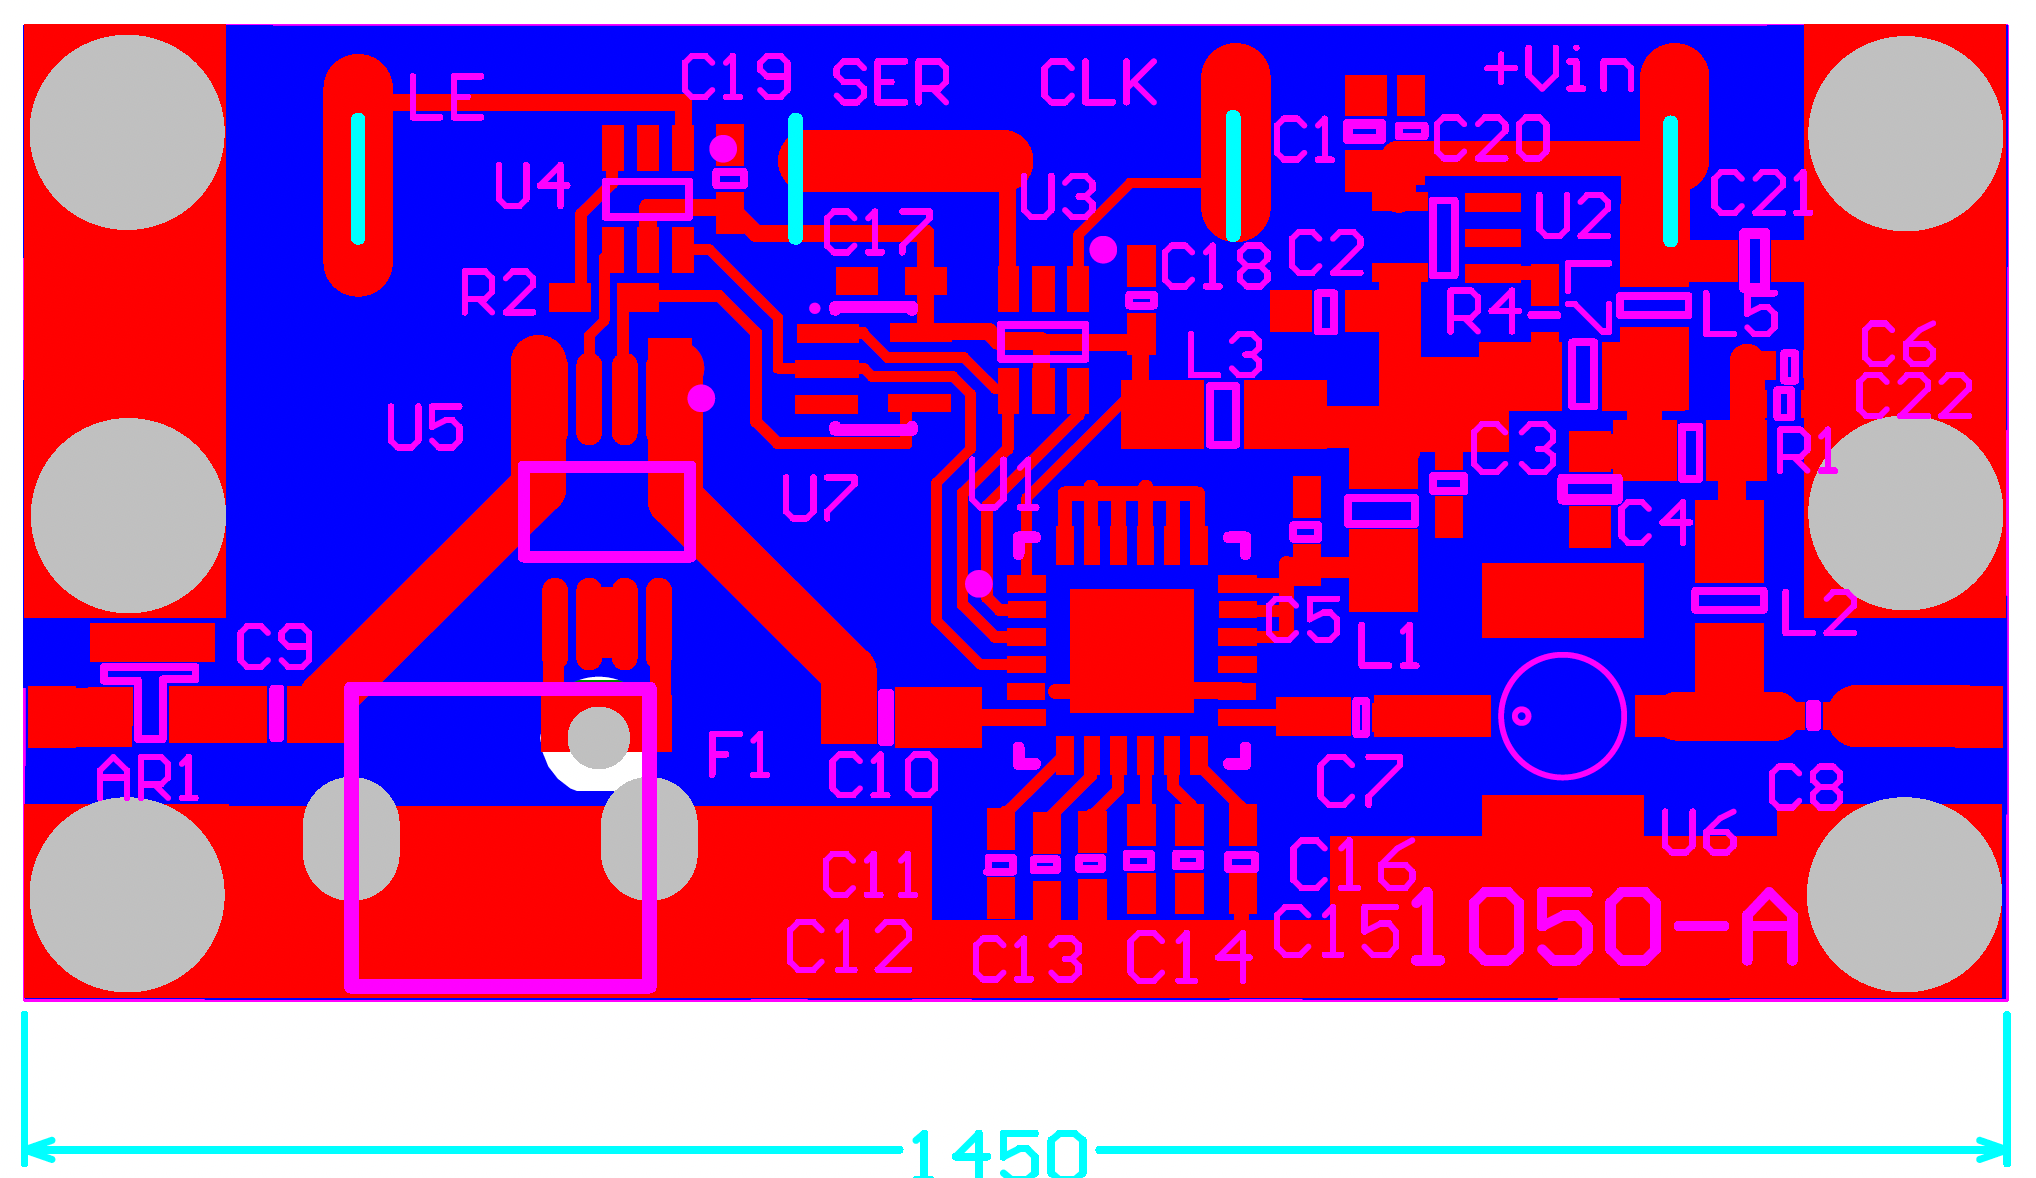
\includegraphics[width=1\linewidth]{Documentation/figures/Attemp_gerber.png}
\caption{1050-A Attemplifier Layout}
\label{fig:Attemp_layout}
\end{figure}
%


\subsection{Wiring}
\label{sec:4.2}
% ----------------------------------------------------------------

There are four 28 awg, twisted wire pairs connected to each attemplifier as shown in Figure \ref{fig:Attemplifier} and \ref{fig:Attemp_pegs}. One wire in each twisted pair is black and functions as the ground for the wire it is twisted with. 

%
\begin{figure}[H]
\centering
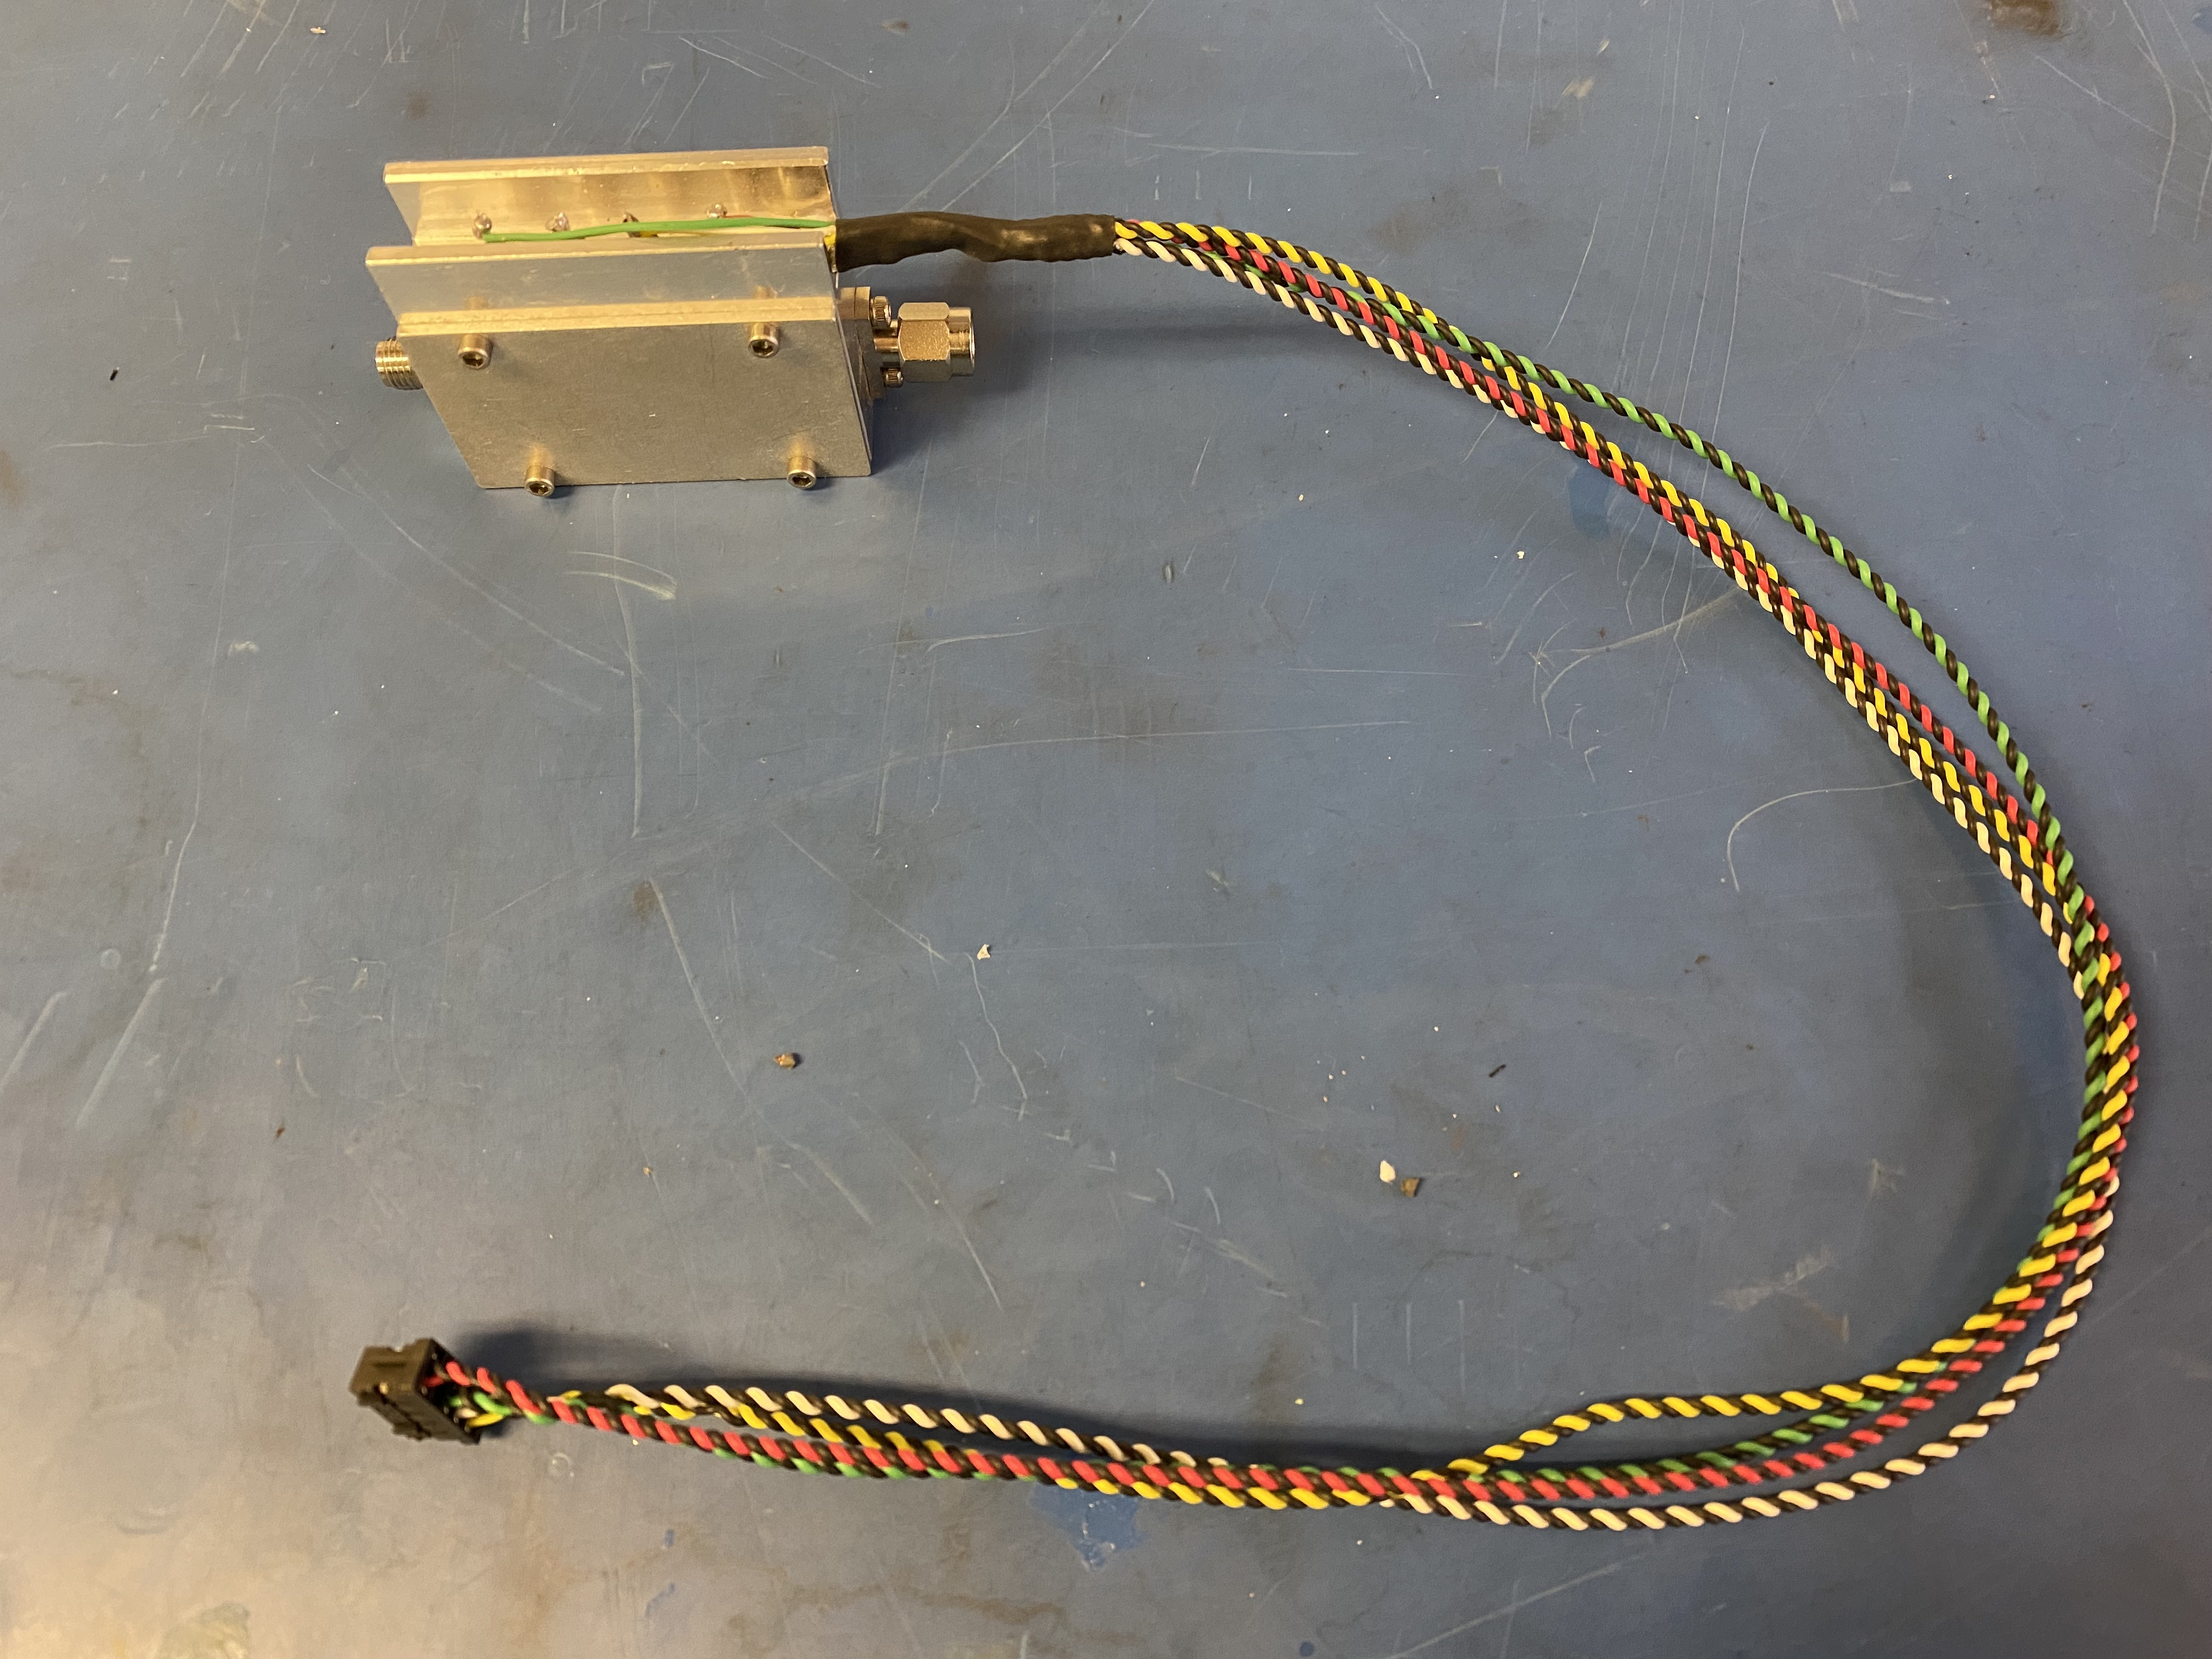
\includegraphics[width=.8\linewidth]{Documentation/figures/Attemplifier.jpeg}
\caption{Attemplifier Complete with Wiring }
\label{fig:Attemplifier}
\end{figure}
%

%
\begin{figure}[H]
\centering
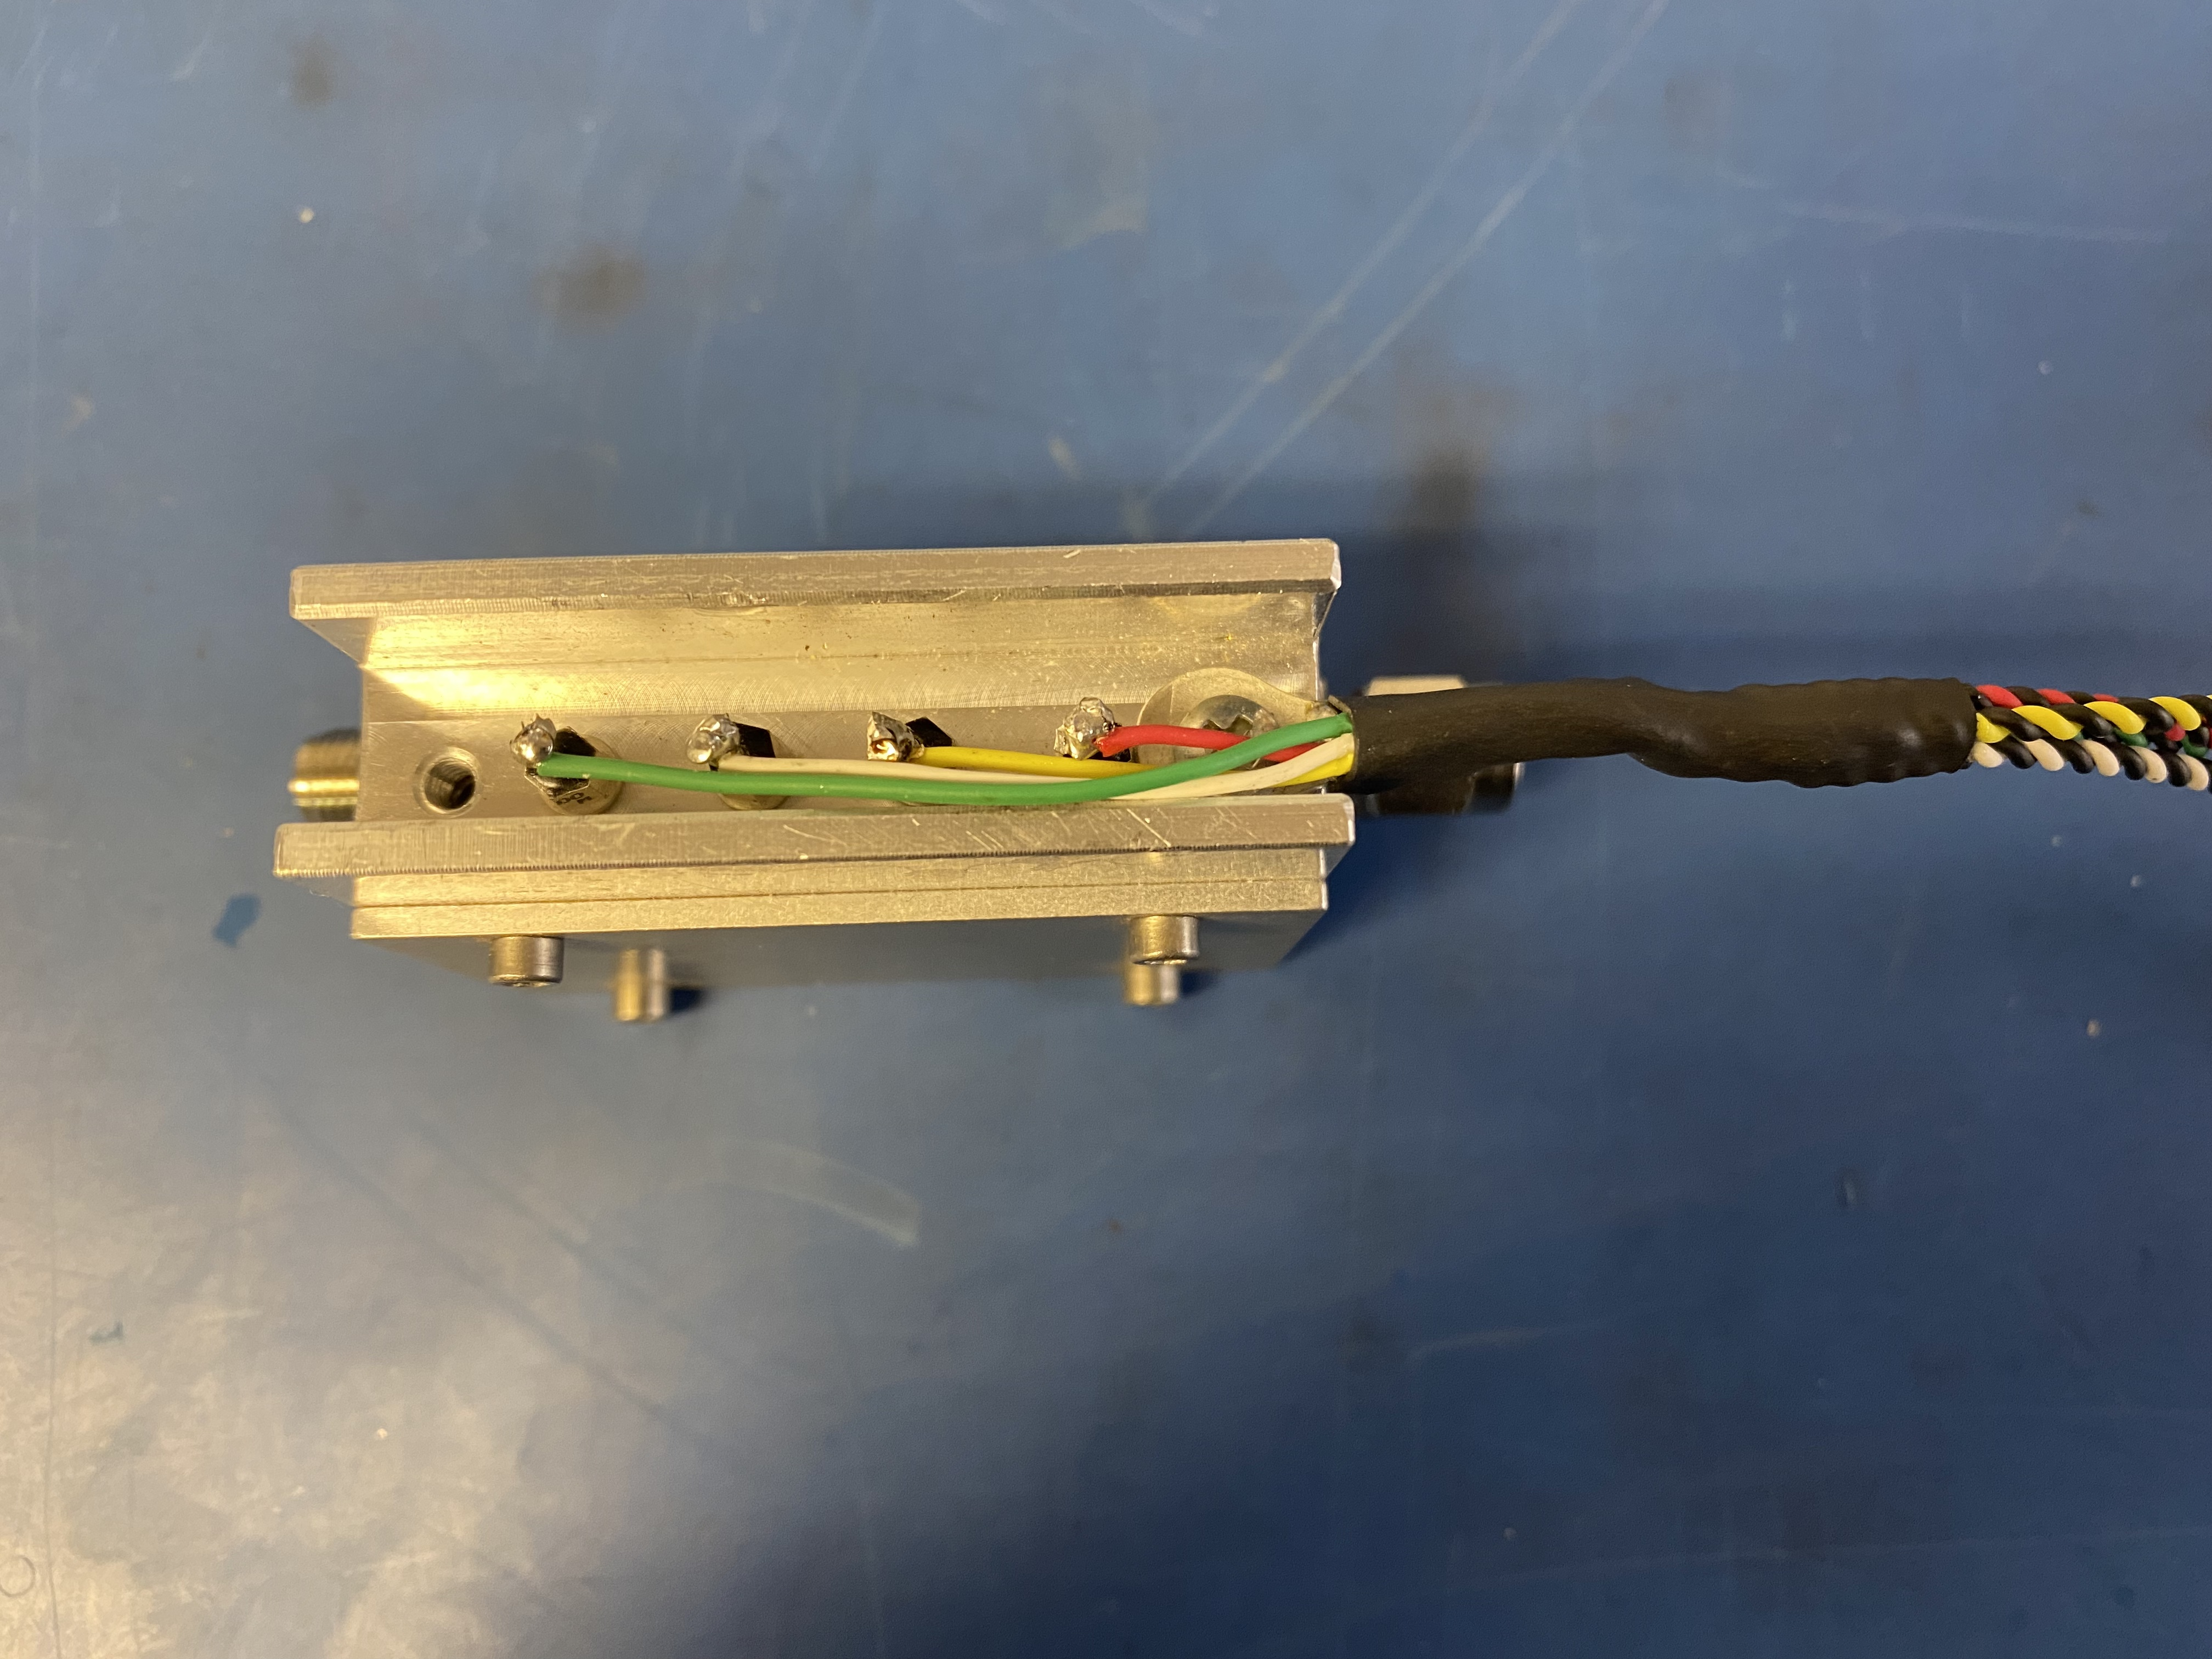
\includegraphics[width=.8\linewidth]{Documentation/figures/Attemp_pegs.jpeg}
\caption{Soldered Wire Connection of an Attemplifier}
\label{fig:Attemp_pegs}
\end{figure}
%

The function of the other four wires is shown in Table \ref{table: Wire_func}. The ground wires are all soldered into a \#6 eye terminal which is screwed into the attemplifier (Figure \ref{fig:Attemp_pegs}). The other wires, meanwhile, are  soldered onto the attemplifier's feed through filters. The order in which they are soldered is shown in Figure \ref{fig:Attemp_pegs}. Note that the wire, solder, and eye terminal for the attemplifiers is considered on hand supplies and therefore are not listed in either of the component lists. 

\begin{table}[H]
\centering
\caption{Attemplifier Wire Functions}
\begin{tabular}{@{}cc@{}}
\toprule
Color & Function\\ 
\midrule
Yellow & Clock\\
White & Data\\
Green & Latch Enable\\
Red & Power\\

\bottomrule            
\end{tabular}
\label{table: Wire_func}
\end{table}

Each of the eight wires ends in a DF11 series crimped contact (PN: DF11-2428SC) that are all then inserted into a DF11 series wire to board header connector (PN: DF11-10DP-2DSA(24)). Figure \ref{fig:pinout} shows the pin out of this connector as viewed from the mating face. The black wire from each twisted pair is directly below its partner in the connector.

%
\begin{figure}[H]
\centering
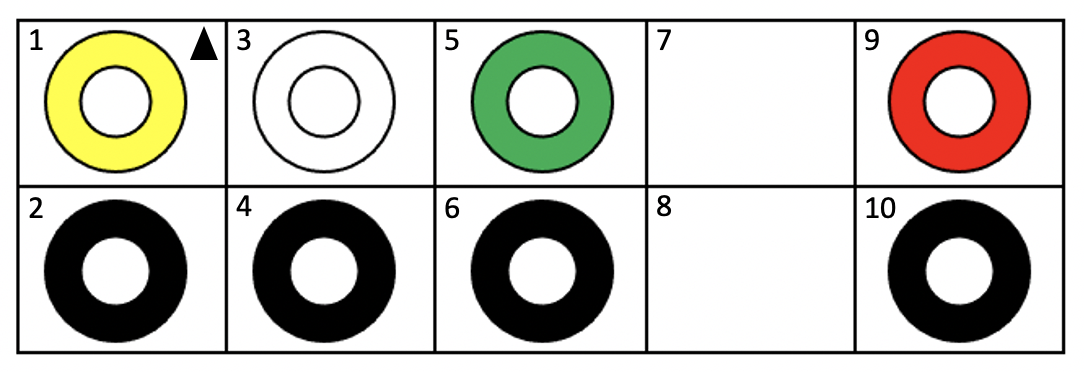
\includegraphics[width=.8\linewidth]{Documentation/figures/Attemp_pinout.png}
\caption{Connector Pin Out of an Attemplifier}
\label{fig:pinout}
\end{figure}
%

\subsection{Testing}
\label{sec:4.3}
% ----------------------------------------------------------------

The attemplifiers were manufactured far prior to the Attemplifier Module being designed. Therefore, before installation, all 352 attemplifiers were tested. The test setup required a N5230C VNA, two male to male SMA cables, female to female adapter, a Raspberry Pi 2 Model B, a control board, a 40 to 40 GPIO Ribbon Cable, a power supply and connector for the Raspberry Pi, a power supply and connector for the control board. Note that the control board's voltage range is 9-25V. To set up the test, the VNA's power is set to -10dBm and the frequency to 10MHz-2GHz.  Then one SMA needs to connected to Port 1 of the VNA on one end and the other to the female terminal on the attemplifer. Next, the second SMA needs to be connected to the VNA's Port 2 and the male terminal on the attemplifier with the female to female adapter in between. Power up the Raspberry Pi and control board and connect them via the 40 to 40 GPIO Ribbon Cable. Finally, plug the attemplifier into P1 of the control board. An image of this test setup is shown in Figure \ref{fig:Attemp_test}. 

%
\begin{figure}[H]
\centering
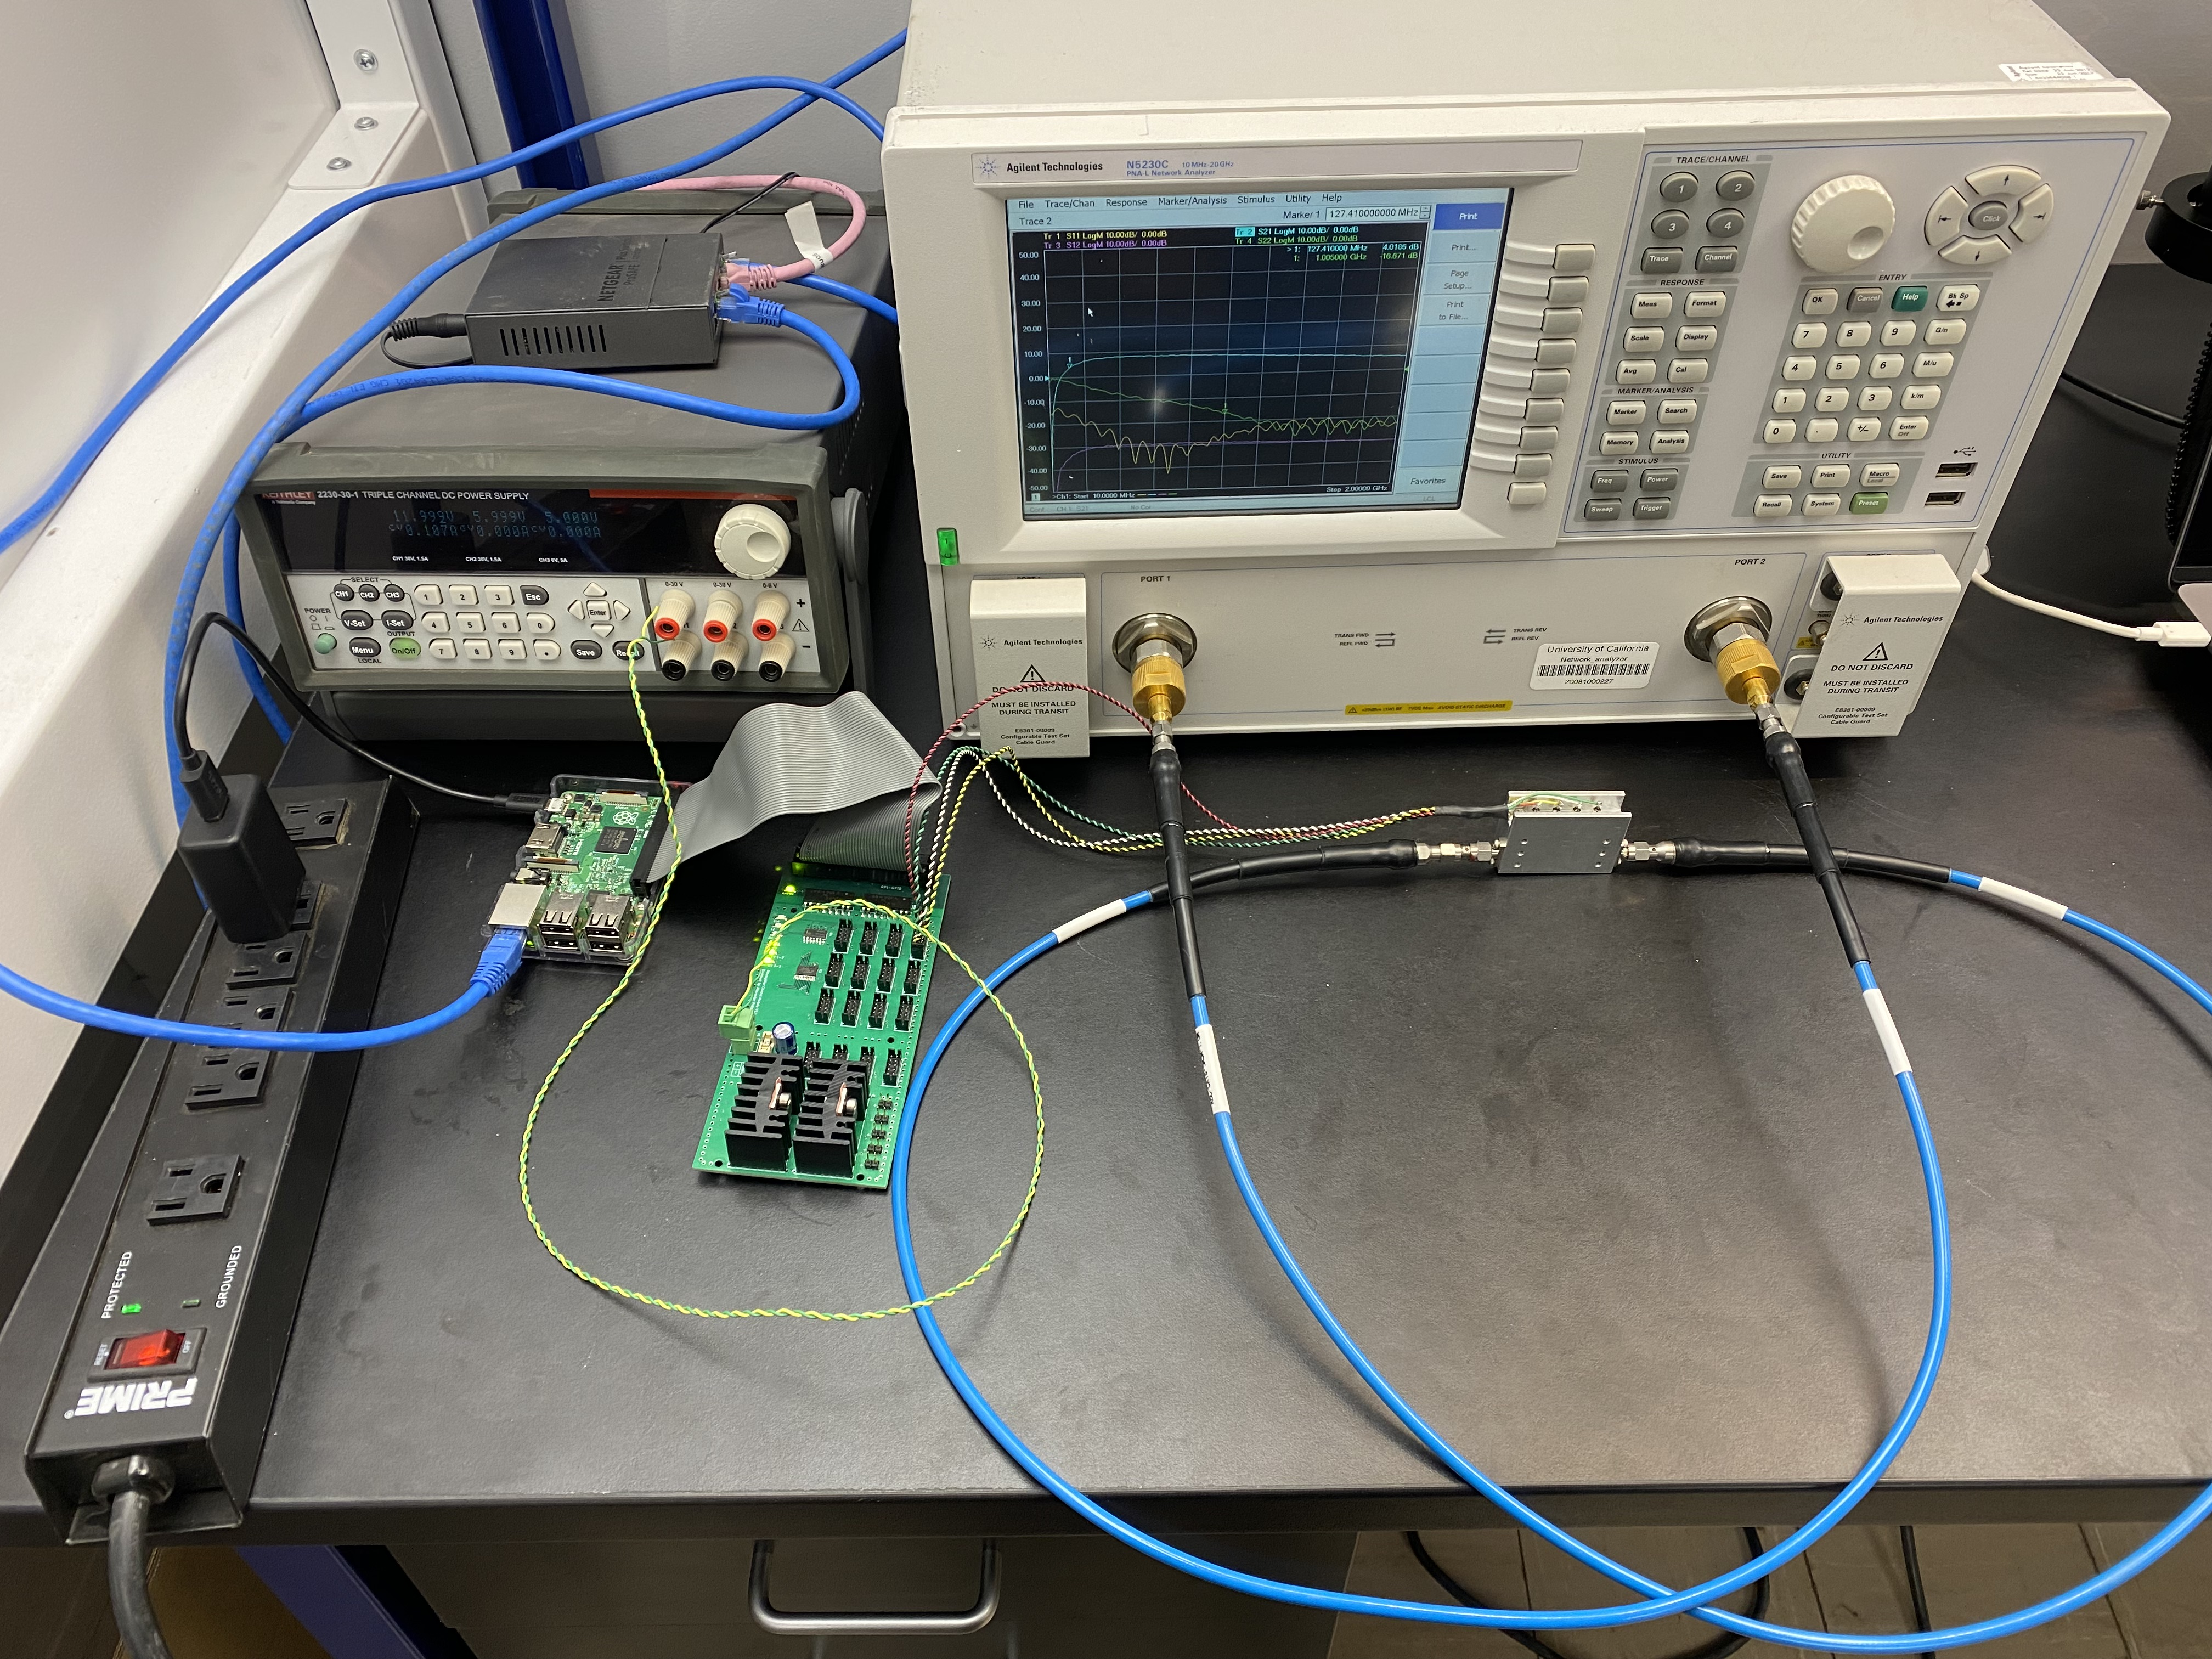
\includegraphics[width=.8\linewidth]{Documentation/figures/Attemp_test.jpeg}
\caption{Set Up to Testing of Indivual Attemplifiers}
\label{fig:Attemp_test}
\end{figure}
%


Commands can now be given through a terminal to set the attenuation of the attmplifier to different values using a script called TestRun. These attenuation changes are displayed on the VNA to show whether the attemplifier is functioning. Below are step-by-step directions on how to test an attemplifier.

\begin{enumerate}
 \item ssh into the Raspberry Pi: ssh sonata@10.1.49.230
 \item Run TestRun script
 \item Watch how the graph on the VNA responds as the attenuation increases. Figure \ref{fig:Test_Run} shows how the VNA display should look as TestRun sets the attenuation to 0dB, 1dB, 2dB, 4dB, 8dB, and 16dB.  Graphs a-f from Figure \ref{fig:Test_Run} match the attenuation settings in ascending order. 

 \item Rate the Attemplifier as pass or fail based on whether its VNA graphs were correct
 
\end{enumerate}

\begin{figure}[H]
 \centering
 
 \begin{subfigure}[b]{.6\linewidth}
   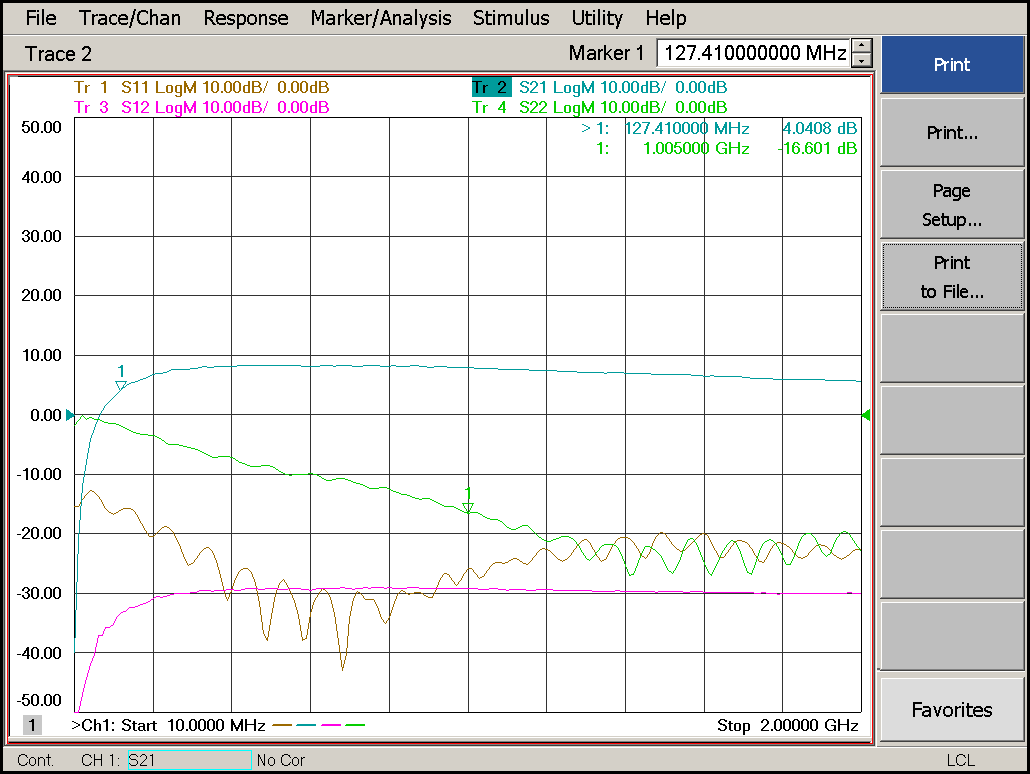
\includegraphics[width=1\linewidth]{Documentation/figures/Attemp_0dB.png}
   \caption{}
   \label{fig:test_0dB}
 \end{subfigure}
 
 \begin{subfigure}[b]{.6\linewidth}
  \centering
   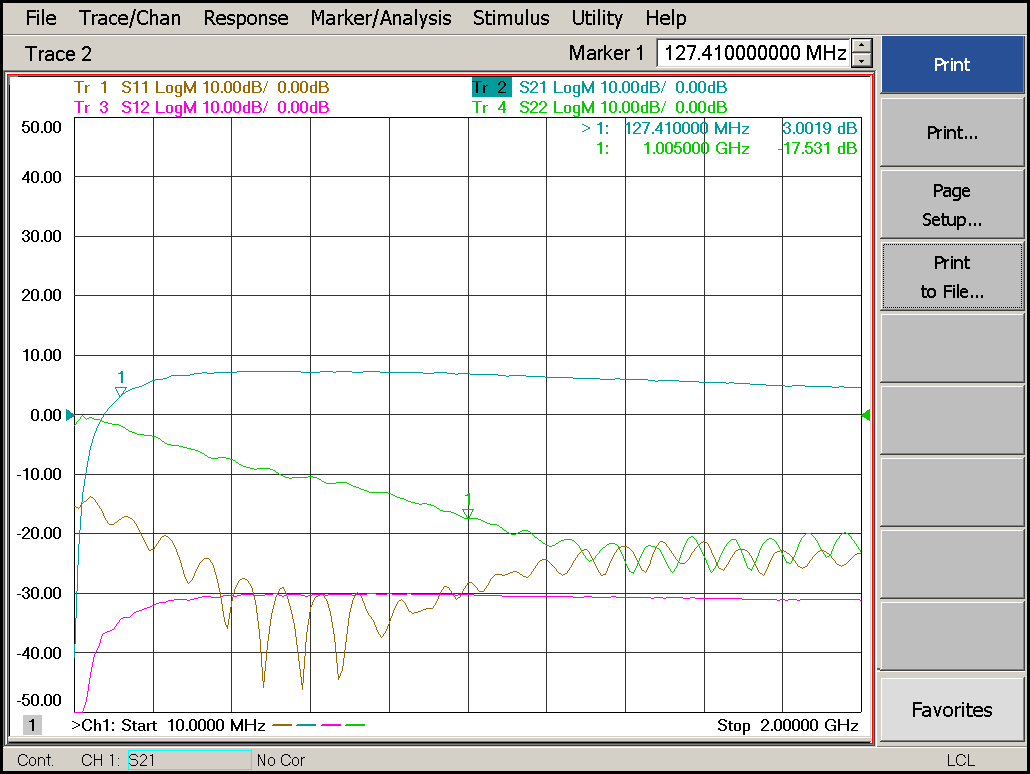
\includegraphics[width=1\linewidth]{Documentation/figures/Attemp_1dB.png}
   \caption{}
   \label{fig:test_1dB}
 \end{subfigure}
 
 \begin{subfigure}[b]{.6\linewidth}
  \centering
  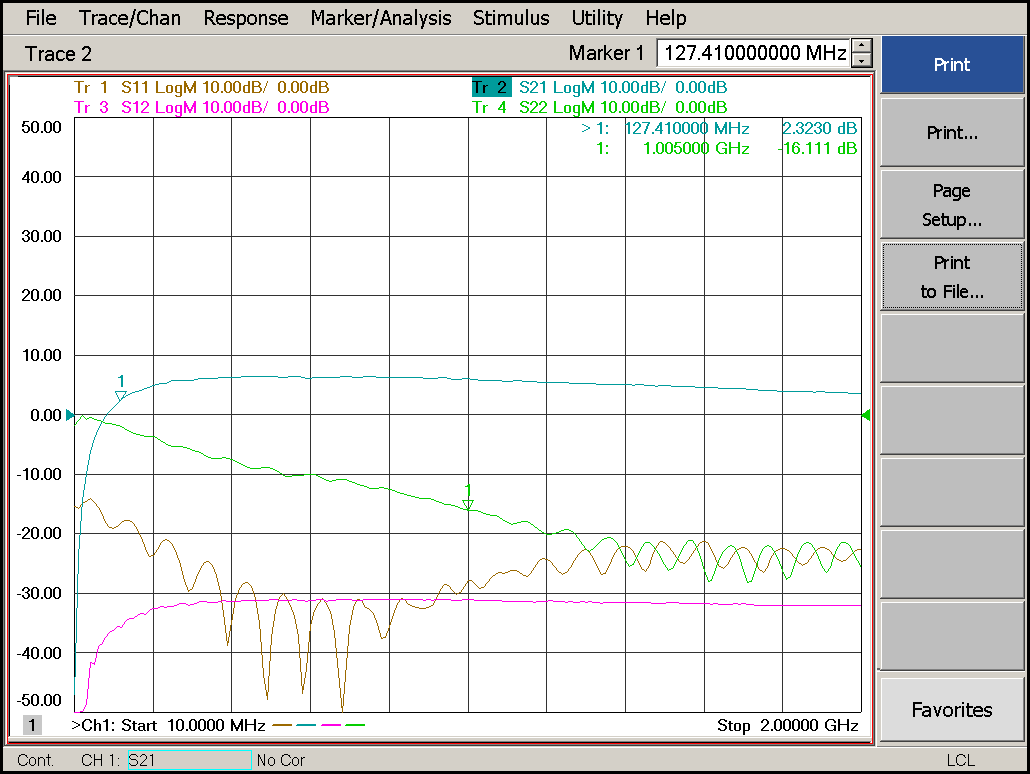
\includegraphics[width=1\linewidth]{Documentation/figures/Attemp_2dB.png}
  \caption{}
  \label{fig:test_2dB}
 \end{subfigure}

\end{figure}

\begin{figure}[H]\ContinuedFloat
 \centering
 
 \begin{subfigure}[b]{.6\linewidth}
   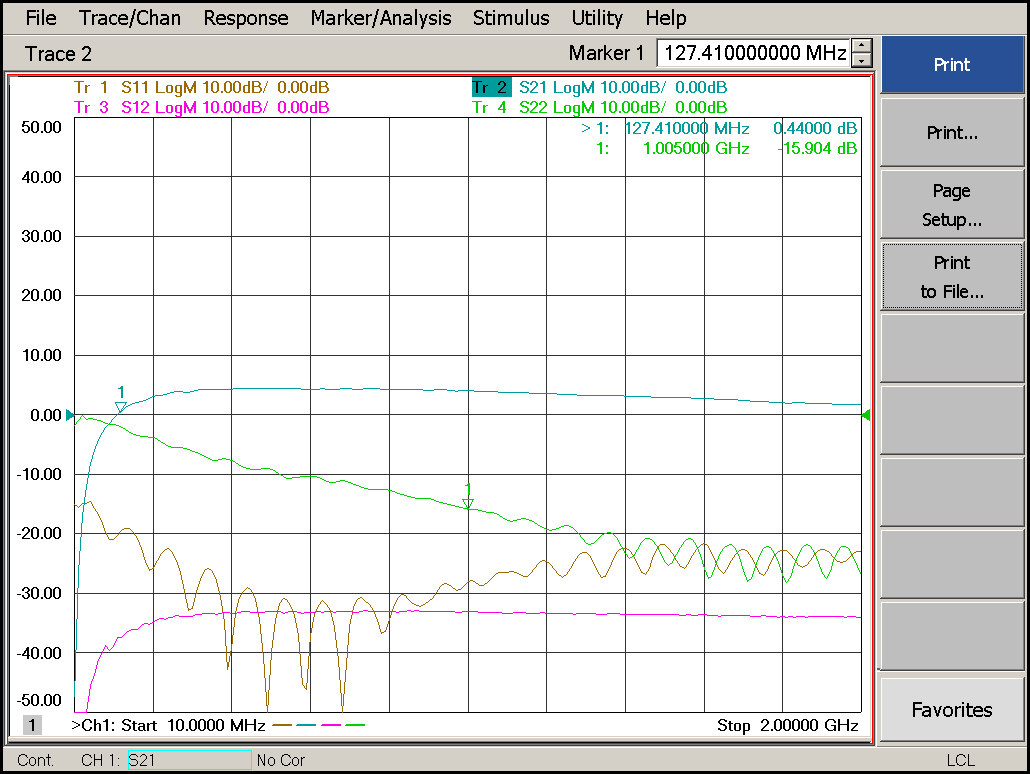
\includegraphics[width=1\linewidth]{Documentation/figures/Attemp_4dB.png}
   \caption{}
   \label{fig:test_4dB}
 \end{subfigure}
 
 \begin{subfigure}[b]{.6\linewidth}
  \centering
   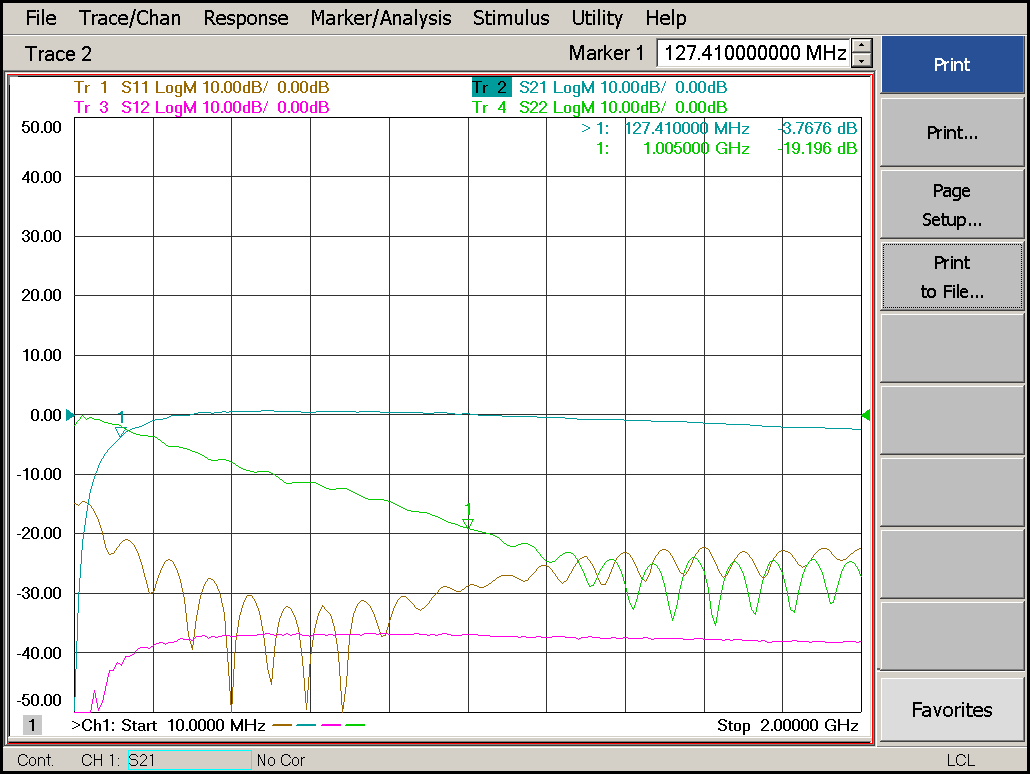
\includegraphics[width=1\linewidth]{Documentation/figures/Attemp_8dB.png}
   \caption{}
   \label{fig:test_8dB}
 \end{subfigure}
 
 \begin{subfigure}[b]{.6\linewidth}
  \centering
  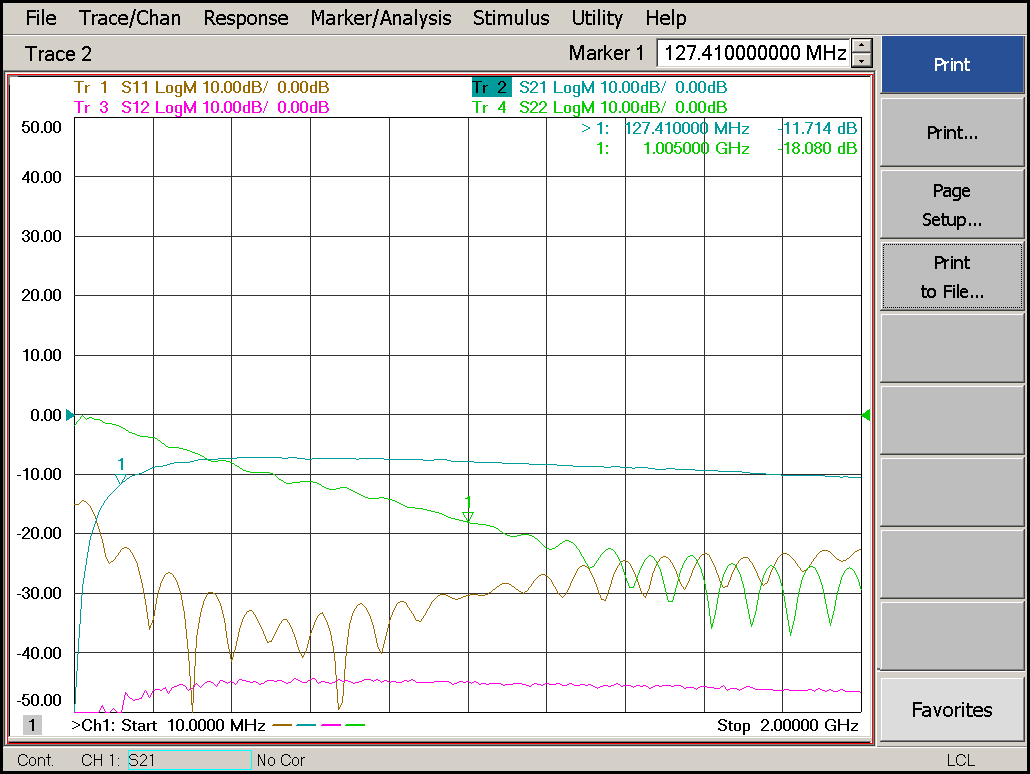
\includegraphics[width=1\linewidth]{Documentation/figures/Attemp_16dB.png}
  \caption{}
  \label{fig:test_16dB}
 \end{subfigure}

 \caption{Desired VNA Displays at all the TestRun Attentions}
 \label{fig:Test_Run}
 
 
\end{figure}

On the VNA display, there are four colored traces. Orange, S11, shows the return loss of the attemplifer's input. Green, S22, shows the return loss of the attemplifer's output. Magenta, S12, shows the transmission from output through the attemplifier and to the input. Cyan, S21, shows the transmission from input through the attemplifier and to the output.  For a functional attemplifier, changing the attenuation changes S21. More specifically, increasing attenuation decreases the power that S21 sits at. This relationship is shown in Figure \ref{fig:Test_Run}. S21 show a gain of 8dB when the attenuation is set to 0dB. The attenuation range of an attemplifier is about 31.5 dB in 0.5 dB steps.



%----------------------------------------------------------------------------------------
%	Power Supplies & Adapter
%----------------------------------------------------------------------------------------
\section{Power Supplies \& Adapter}
\label{sec:6}
% ----------------------------------------------------------------

There are two power supplies in the Attemplifier Modules. The first, called the general linear power supply, is a Schroff PSG 112 (PN: 13105-012) and is mounted directly to the front panel of the enclosure. It powers the control board, the attemplifiers, and the fan (PN: PF80251V1-1000U-A99). The operating temperature range of the power supply is from $0^{\circ}$C through $70^{\circ}$C and the technical specifications are shown in Table \ref{tab:gen_psu_spec}. As shown in the table, this linear power supply can only be operated at $110 \rm{VAC}$, so \emph{only operate the module at 110 VAC.}

The second power supply, called the Rasberry Pi power supply, is a Mean Well RS-15-5 (PN: RS-15-5) and is mounted directly behind the first power supply. This power supply powers only the Raspberry Pi. It operates at a temperature range of $-20^{\circ}$C through $70^{\circ}$C. The technical specification are shown in Table \ref{tab:ras_psu_spec}. The power entry module (PN: 43,044,005), mounted in the back panel, combines an IEC inlet and a mains filter with a single fuse holder. The AC supply fuse (PN: 0217001.HXP) current rating for this unit is selected to be 1\,A. 

\begin{table}[H]
\centering
\caption{General Linear Power Supply Specification}
\label{tab:gen_psu_spec}
\begin{tabular}{@{}ccccc@{}}
\toprule
\multicolumn{1}{l}{Description} & \multicolumn{1}{l}{Output Voltage} & \multicolumn{1}{l}{Output Current} & \multicolumn{1}{l}{Power W} & \multicolumn{1}{l}{Input Voltage} \\ \midrule
PSG 112                        & 12\,VDC                               & 4.2A                               & 50W                         & $110\rm{VAC}$                              \\ \bottomrule
\end{tabular}
\end{table}

\begin{table}[H]
\centering
\caption{Rasberry Pi Power Supply Specification}
\label{tab:ras_psu_spec}
\begin{tabular}{@{}ccccc@{}}
\toprule
\multicolumn{1}{l}{Description} & \multicolumn{1}{l}{Output Voltage} & \multicolumn{1}{l}{Output Current} & \multicolumn{1}{l}{Power W} & \multicolumn{1}{l}{Input Voltage} \\ \midrule
RS-15-5                        & 5\,VDC                               & 3A                               & 15W                         & $85 \sim 164\,\rm{VAC}$                              \\ \bottomrule
\end{tabular}
\end{table}



%----------------------------------------------------------------------------------------
%	Module Wiring
%--------------------------------------------------------------------------------------

\section{Module Wiring}
\label{sec:6}
% ----------------------------------------------------------------

This section outlines the internal connections of the Attemplifier Module. It is broken up into how parts connect to the front panel, the control board, the Raspberry Pi, the power supplies, and the power entry module. 

\subsection{Front Panel}      
\label{sec:6.1}
% ----------------------------------------------------------------

 For the front panel (PN: ATA-AP-2456717498.fpd), an IN and OUT connection of same number connect to an attemplifier which in turn connects to the control board. The IN connectors hook up to the female inlets on the attmplifiers via a nine inch male to female SMA cable (PN: PE39433-9). The OUT connectors hook up to the male inlets of the attemplifiers via a twelve inch male to female SMA cable (PN: PE39433-12) with a female to female adapter in between (PN; PE9070). Note that the attemplifier numbers are different for each module as there are 352 attemplifiers. The attemplifiers are installed in each module in groups of sixteen in ascending order. For example, module 1 has attemplifiers 1-16, module 2 has attemplifiers 17-32, module 3 which has attemplifiers 33-48, and so on. Thus, while Table \ref{tab:Front_to_attemp} only shows the front panel cable connections for module 1, it is representative for all of the modules.



\begin{table}[H]
\centering
\caption{Front Panel Cable Connections for Module 1}
\begin{tabular}{@{}cc@{}}
\toprule
Panel Labels & Attemplifier Number\\ 
\midrule
IN-1 \& OUT-1 & 1\\
IN-2 \& OUT-2 & 2\\
IN-3 \& OUT-3 & 3\\
IN-4 \& OUT-4 & 4\\
IN-5 \& OUT-5 & 5\\
IN-6 \& OUT-6 & 6\\
IN-7 \& OUT-7 & 7\\
IN-8 \& OUT-8 & 8\\
IN-9 \& OUT-9 & 9\\
IN-10 \& OUT-10 & 10\\
IN-11 \& OUT-11 & 11\\
IN-12 \& OUT-12 & 12\\
IN-13 \& OUT-13 & 13\\
IN-14 \& OUT-14 & 14\\
IN-15 \& OUT-15 & 15\\
IN-16 \& OUT-16 & 16\\

\bottomrule            
\end{tabular}
\label{tab:Front_to_attemp}
\end{table}

\subsection{Control Board}
\label{sec:6.2}
% ----------------------------------------------------------------

The control board is connected to the general power supply (PN: 13105-012), the Raspberry Pi (PN: RPI2-MODB-V1.2), the LEDs (PN: Q6F7BXXB02E and Q6F3GXXY02E), and the attemplifiers.

For the power supply connection, a twisted pair of red and black 18 awg wire was made. Then two E7508 gray ferrules were crimped onto one end and inserted into a 2 way cable mount screw terminal (PN: 1803578). This then plugs into the straight PCB terminal block header (PN: 1803426) on the control board. Because the ferrules and wire are considered on hand supplies, they are not included on either of the components lists. 

The Raspberry Pi is connected to the control board only via a 40 to 40 GPIO Ribbon Cable. It plugs into a 40 circuit C-Grid Header (PN: 70246-4001)

There are sixteen DF11 series wire to board receptacles (PN: DF11-10DS-2C) on the control board. Each one matches to an attemplifier. Table \ref{tab:Attemp_to_board} shows how they do so for module 1. However, no matter the module, the attemplifier with the lowest number always plugs into P1 and then proceeds in ascending order. 

\begin{table}[H]
\centering
\caption{Front Panel Cable Connections for Module 1}
\begin{tabular}{@{}cc@{}}
\toprule
Attemplifier Number & Board Label\\ 
\midrule
1 & P1\\
2 & P2\\
3 & P3\\
4 & P4\\
5 & P5\\
6 & P6\\
7 & P7\\
8 & P8\\
9 & P9\\
10 & P10\\
11 & P11\\
12 & P12\\
13 & P13\\
14 & P14\\
15 & P15\\
16 & P16\\

\bottomrule            
\end{tabular}
\label{tab:Attemp_to_board}
\end{table}

The control board has five two pin Straight PCB Headers (PN: 22-28-4023) for each LED on the front panel. The control board was miss labeled, so the front panel label does not necessarily match the control board label (Table \ref{LED_to_board}). 

\begin{table}[H]
\caption{LED Internal Cable Connections}
\centering
\label{LED_to_board}
\begin{tabular}{@{}cc@{}}
\toprule
 LED Panel Label & Board Connector Label\\ 
\midrule
5 V 1-2 & 5 V 1-2\\
5 V 2-2 & 5 V 2-2\\
CLK & DATA\\
DATA & CLK\\
LE & LE\\

\bottomrule            
\end{tabular}
\label{table:LED_to_board}
\end{table}

The LEDs themselves had their wires extended with 28 awg red and black wire. Again, the wire is not listed in the component lists because it is considered to be an on hand material. Both wires where then crimped with a F/M crimp term (PN: M20-1180042) contact and then inserted into a 2 pin SIL housing (PN: M20-1060200). The LED headers on the control are also labeled with + and -. Each LED's red wire plugs into the + pin and the black plugs into the -.

\subsection{Raspberry Pi}
\label{sec:6.3}
% ----------------------------------------------------------------

The Raspberry Pi (PN: RPI2-MODB-V1.2) is connected to the Raspberry Pi power supply (PN: 	RS-15-5), the Ethernet feed through (PN: XB5PRJ45), and the control board. For the connection to the Raspberry Pi power supply, the USB 2.0 connection cable is used. Prior to connecting up, the cable needs to be modified: the five pin female connector needs to be removed, all the wires except the black and red need to be shortened and isolated, and finally a CLS series fork terminal (PN: CLS-TV-1806) soldered onto the red and black wire individually. The Ethernet feed through connects to the Raspberry Pi via a one foot Cat6 Ethernet cable (PN: C6-UTPSGPVCBE-0.3M). 

\subsection{Raspberry Pi Power Supply}
\label{sec:6.4}
% ----------------------------------------------------------------

The Raspberry Pi power supply (PN: RS-15-5) is connected to the Raspberry Pi (PN: RPI2-MODB-V1.2), the base plate (PN: ATA-AP-2456717499.fpd), and the power supply entry module (PN: 43,044,005). Refer to Figure \ref{fig:Attemp_Power_Schematic} for the wiring schematic of the Raspberry Pi power supply. 

On the lower voltage side of the power supply, the modified USB 2.0 connection cable connects the Raspberry Pi and the Raspberry Pi power supply. The USB end plugs into the Raspberry Pi while the CLS series fork terminal (PN: CLS-TV-1806) connect to the power supply. The lower voltage side of the power supply is NOT connected to the base plate for grounding. This leaves the Raspberry Pi floating to minimize interference.

On the mains voltage end of the power supply, it is wired up to the power entry module and the base plate. The green, white, and black wires all connect to the power supply via CLS series fork terminal. The green wire connects to the base plate via a 6s  eye terminal. The white and black wires then end in female quick disconnect terminals (PN: FDFD1-250) to connect to the power supply entry module.

\subsection{The General Linear Power Supply}
\label{sec:6.5}
% ----------------------------------------------------------------

The general liner power supply (PN: 13105-012) is connected to the control board, the fan (PN: PF80251V1-1000U-A99), the base plate (PN: ATA-AP-2456717499.fpd), and the power supply entry module (PN: 43,044,005). Refer to Figure \ref{fig:Attemp_Power_Schematic} for the wiring schematic of the general linear power supply. 

For the lower voltage side of linear power supply, it connects to the control board, the fan, and the base plate. As mentioned in a previous section, a twisted pair of 18 awg wire with ferrule plugged into a 2 way cable mount screw terminal (PN: 1803578) connects to the control board while the other end connects to the linear power supply. The fan, the wires of which were extended with 20 awg red and black wire, also plugs into linear power supply. Note that the linear power supply's wire bridge's are made out of 18 awg. The lower voltage end is grounded in this case with the green wire that screws into the base plate via s 6s eye terminal. Finally, the terminals for +V, -V, and -Sense are female piggyback disconnect terminal (PN: PBDD2-250) while +Sense has a female quick disconnect terminal (PN: FDFD1-250).

For the mains voltage end, the linear power supply is connected to the power entry module and the base plate. The green, black, and white wires all connect to the linear power supply via female quick disconnect terminals. Like the other grounding wire, the green wire has a 6s eye terminal that is screwed into the base plate. Lastly, the white and black wires plug into the power entry module via female piggyback disconnect terminals.

\subsection{The Power Entry Module}
\label{sec:6.5}
% ----------------------------------------------------------------

The power entry module (PN: 43,044,005) is connected to the base plate (PN: ATA-AP-2456717499.fpd), the general power supply (PN: 13105-012), and the Raspberry Pi power supply (PN: RS-15-5). Refer to Figure \ref{fig:Attemp_Power_Schematic} for the wiring schematic of the power entry supply. 

The green ground wire plugs into the power entry module via a
female quick disconnect terminal (PN: FDFD1-250) while the other end has 6s eye terminal that is screwed into the base plate. Then the white and black wires from the Raspberry Pi power supply plug into the female piggyback disconnect terminals (PN: PBDD2-250) from the black and white wires of the general linear power supply. Finally, the general linear power supply wires plug into the power entry module.

\begin{figure}[H]
\centering
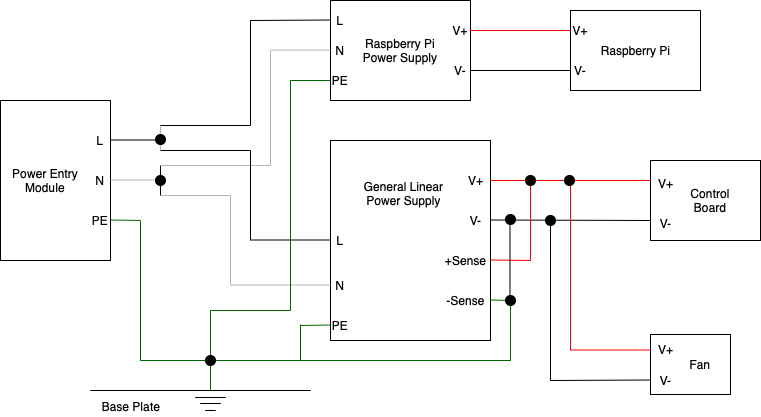
\includegraphics[width=1\linewidth]{Documentation/figures/Attemp_Power_Schematic.png}
\caption{Attemplifier Module Power Schematic. The colors of the connections represent the color of wire used. The grey represents white wire. All the wires connecting the to the power entry module and base plate are 12 awg. The rest of the wire gauges are specified  in the power supply subsections.}
\label{fig:Attemp_Power_Schematic}
\end{figure}

%----------------------------------------------------------------------------------------
%	Completed Module
%----------------------------------------------------------------------------------------
\section{Completed Module}
\label{sec:7}
% ----------------------------------------------------------------

Upon completion, an assembled Attemplifier Module is shown in the figures below. The biggest difference between the finished module and the CAD design is the wiring as the CAD design did not include wiring. Furthermore, the fully completed module includes a lid, as shown in Figure \ref{fig:Module_w/_lid}, but was absent in Figures \ref{fig:CAD-Iso} and \ref{fig:CAD-above}.


\begin{figure}[H]
\centering
\includegraphics[width=1\linewidth]{Documentation/figures/Top view.jpeg}
\caption{Completed Attemplifier Module}
\label{fig:Module_above}
\end{figure}

\begin{figure}[H]
\centering
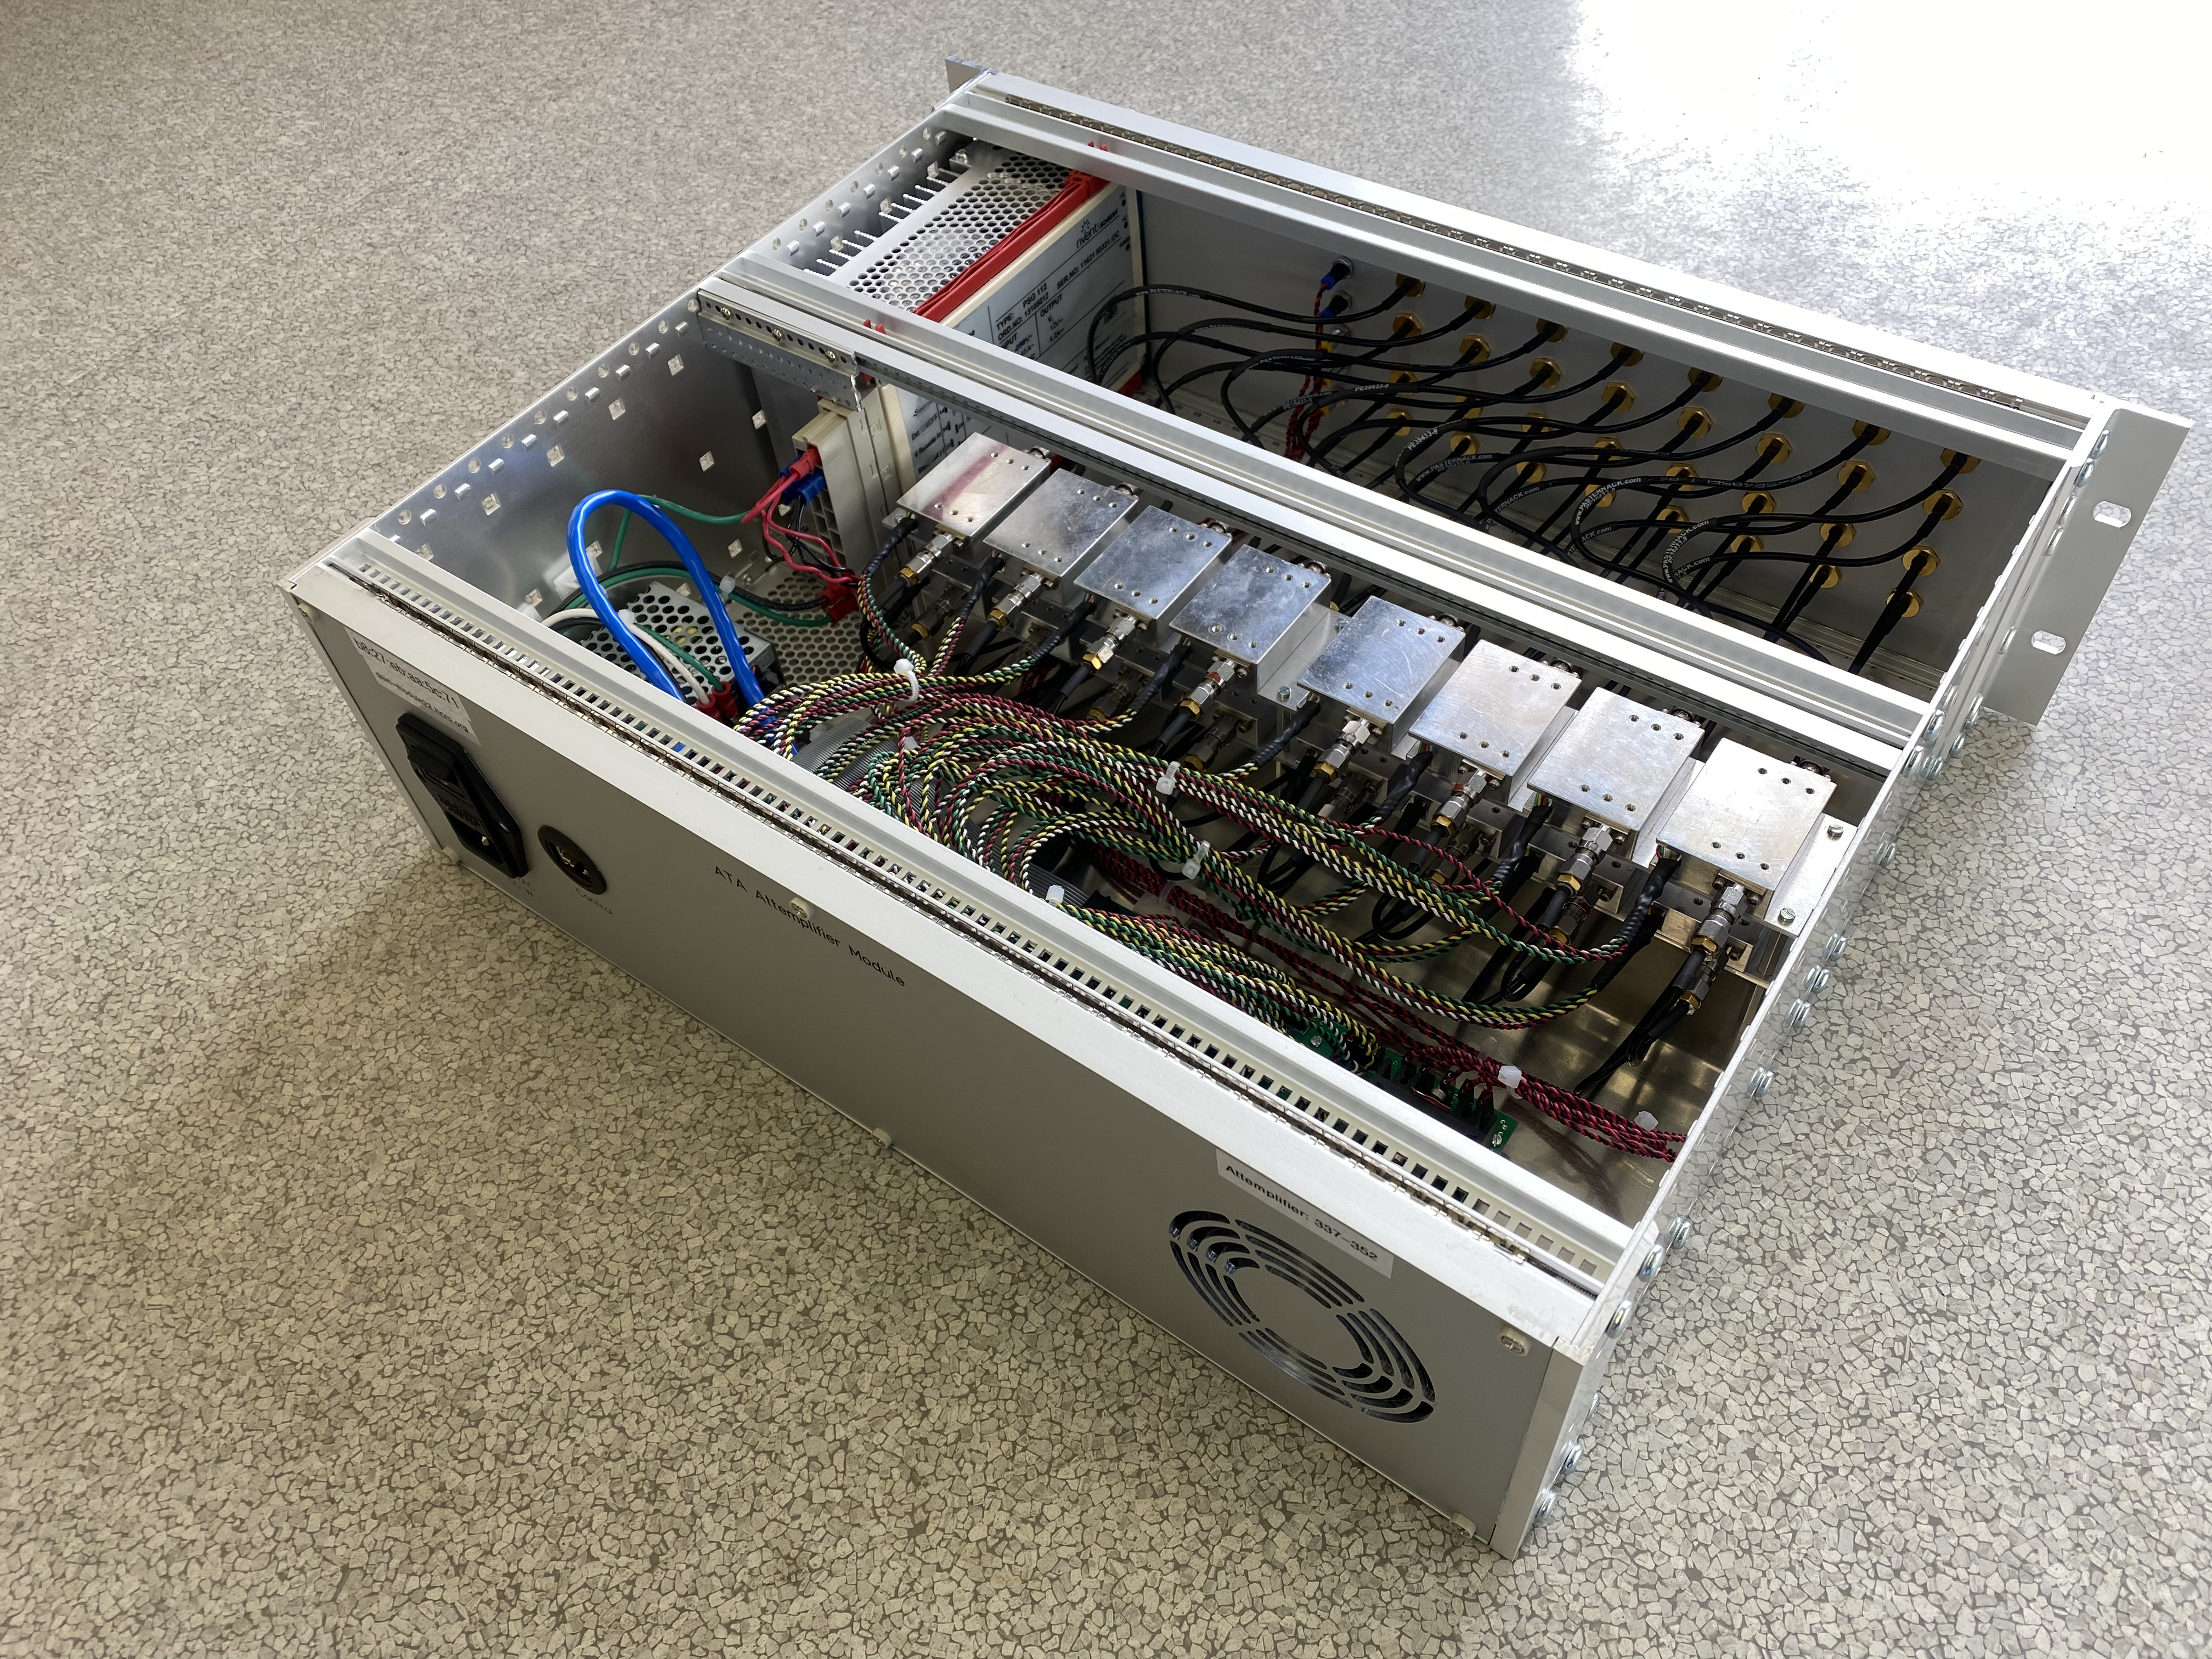
\includegraphics[width=.9\linewidth]{Documentation/figures/backpanel.jpeg}
\caption{Back Panel of Completed Attemplifier Module}
\label{fig:Module_back}

\hfill \break
\hfill \break

\centering
\includegraphics[width=.9\linewidth]{Documentation/figures/lid.jpeg}
\caption{Completed Attemplifier Module with Lid}
\label{fig:Module_w/_lid}
\end{figure}

\newpage

%----------------------------------------------------------------------------------------
%	Module Testing
%----------------------------------------------------------------------------------------
\section{Module Testing}
\label{sec:8}
% ----------------------------------------------------------------

This section describes the testing that each Attemplifier Module went through before it was deemed ready for installation. The test setup, test method, desired results, and encountered problems will all be specifically outlined. Note that the setup, method, and desired results are essentially the same to the prior testing done for each individual attemplifier.

\subsection{Setup}
\label{sec:8.1}
% ----------------------------------------------------------------

For the test setup, a N5230C VNA along with two male to male SMA cables are required. The Attemplifier Module needs to be plugged into power, connected to the network, and turned on. Next, the VNA needs power is set to -10dBm and the frequency to 10MHz-2GHz. Finally, the SMA cables must be connected up: one from PORT 1 on VNA to an IN feed through and the other from PORT 2 on the VNA to the OUT feed through of the same number as the IN. An image of the setup is shown in Figure \ref{fig:Test_Setup}.

 \begin{figure}[H]
 \centering
 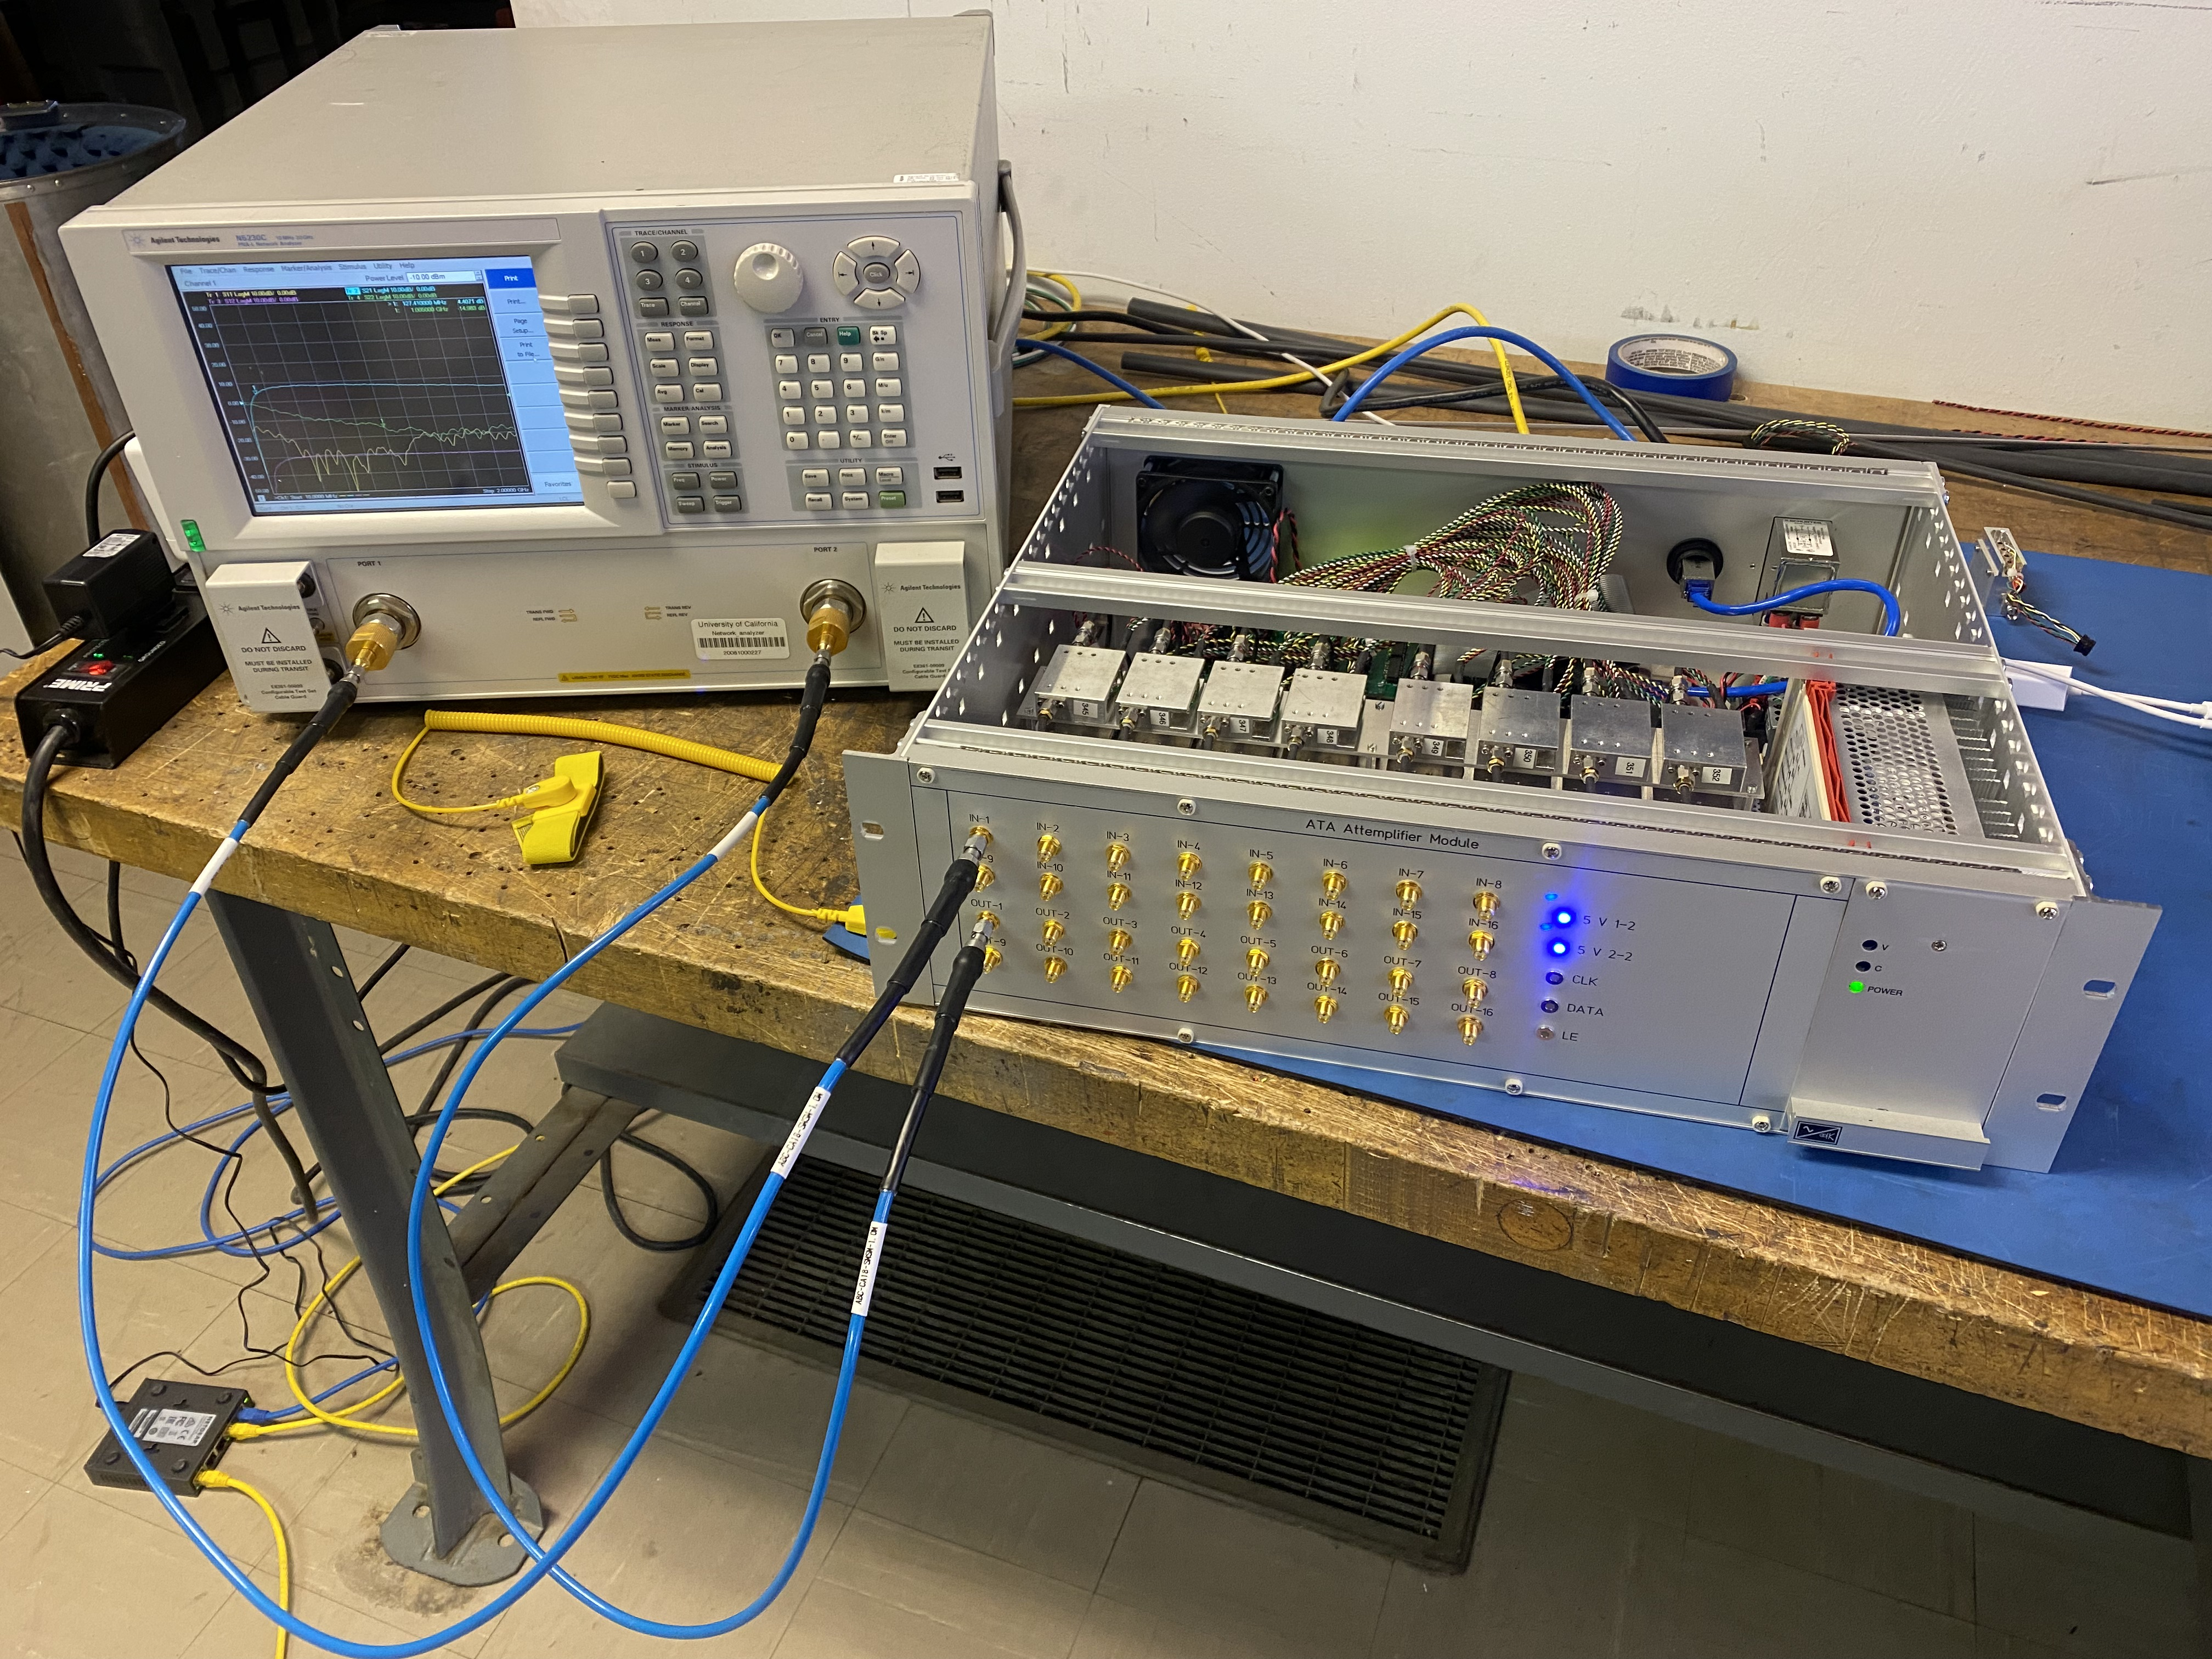
\includegraphics[width=1\linewidth]{Documentation/figures/Test_setup.jpeg}
 \caption{Attemplifier Module Test Setup}
 \label{fig:Test_Setup}
 \end{figure}

\subsection{Method \& Desired Results}
\label{sec:8.2}
% ----------------------------------------------------------------

To test the module, each attemilifer must be tested individually. As discussed in the previous section, this is done by connecting SMA cables from the VNA to the respective pair of IN and OUT feed through of the attemplifier being tested. Once done, commands are given through a terminal to set the attenuation of the attemplifier to three different values. The results of these attenuation settings are displayed on the VNA and show whether the attemplifier is working properly. Below are the set of terminal commands used to test each attemplifier along with the desired results displayed on the VNA.

\begin{enumerate}
 \item ssh into the module: ssh sonata@gain-module1.hcro.org \\
  The number in the ssh command changes based on which module you are testing. Before the attemplifier is set to an attenuation, the VNA should have the display in Figure \ref{fig:Before_atten}.
  
 \begin{figure}[H]
 \centering
 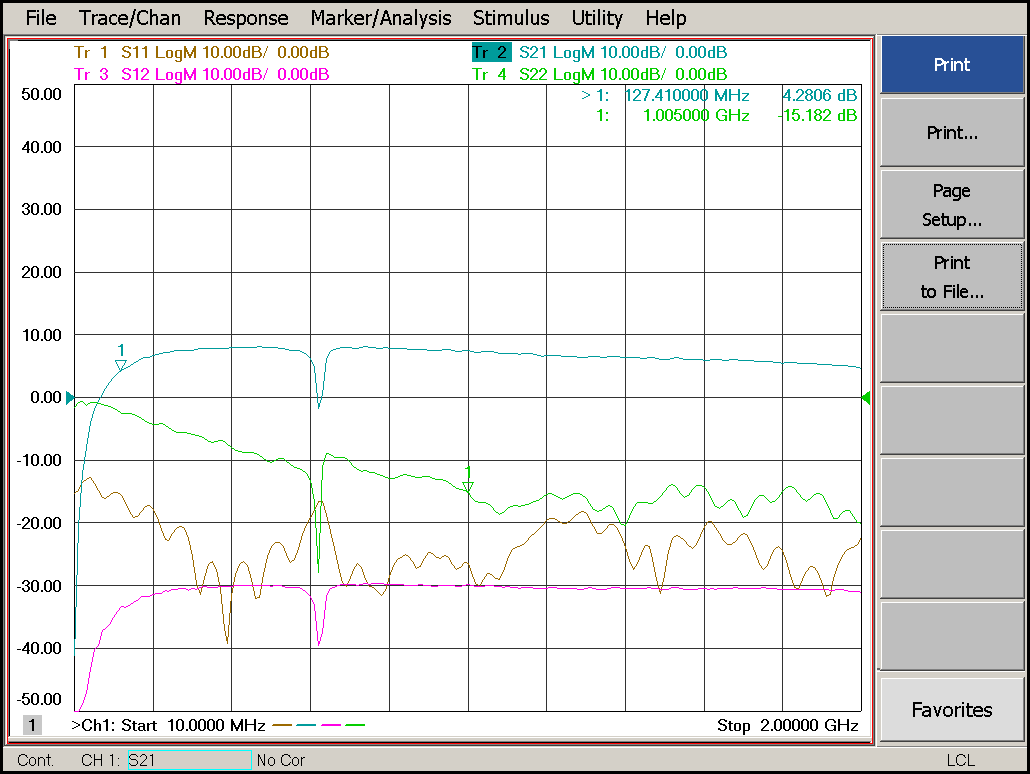
\includegraphics[width=.9\linewidth]{Documentation/figures/Before_set.png}
 \caption{VNA Display before Attenuation is Set}
 \label{fig:Before_atten}
 \end{figure}
 
 \item select the attemplifier and set its attenuation to 0: Attemplifier -n 1 -a 0
 
 \begin{figure}[H]
 \centering
 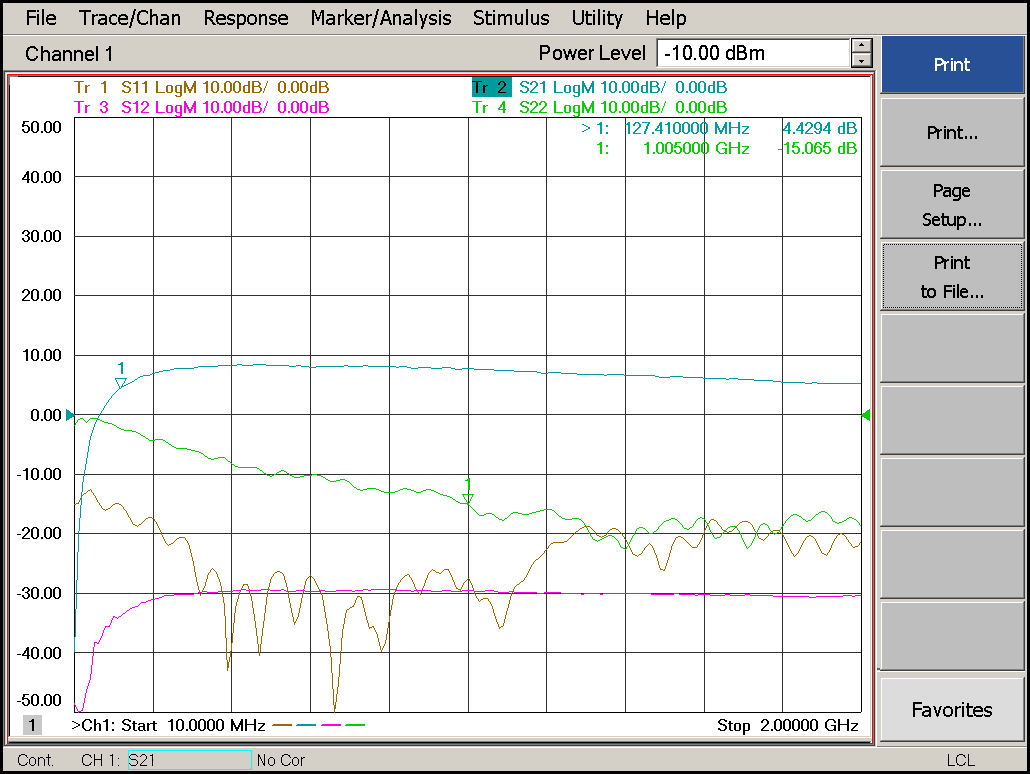
\includegraphics[width=.9\linewidth]{Documentation/figures/Correct_0_atten.png}
 \caption{Desired VNA Display for 0 Attenuation}
 \label{fig:Attenuation_0}
 \end{figure}

 \item set the attenuation to 10: Attemplifier -n 1 -a 10
 
 \begin{figure}[H]
 \centering
 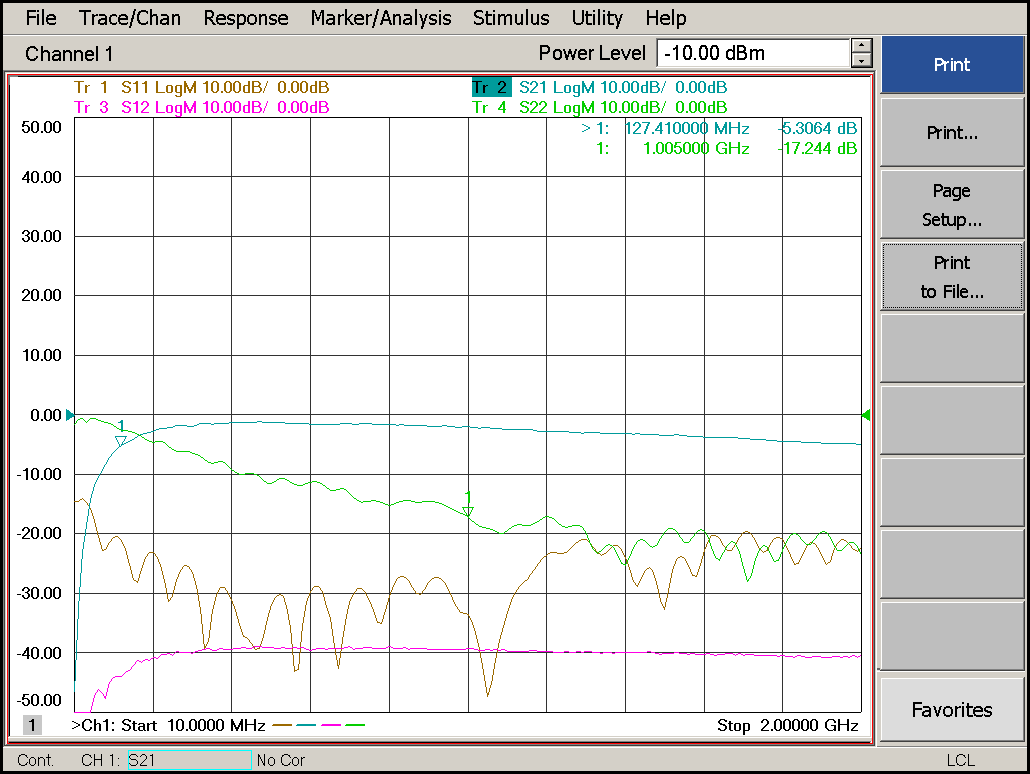
\includegraphics[width=.9\linewidth]{Documentation/figures/Correct_10_atten.png}
 \caption{Desired VNA Display for 10 Attenuation}
 \label{fig:Attenuation_10}
 \end{figure}

 \item set the attenuation to 20: Attemplifier -n 1 -a 20
 
 \begin{figure}[H]
 \centering
 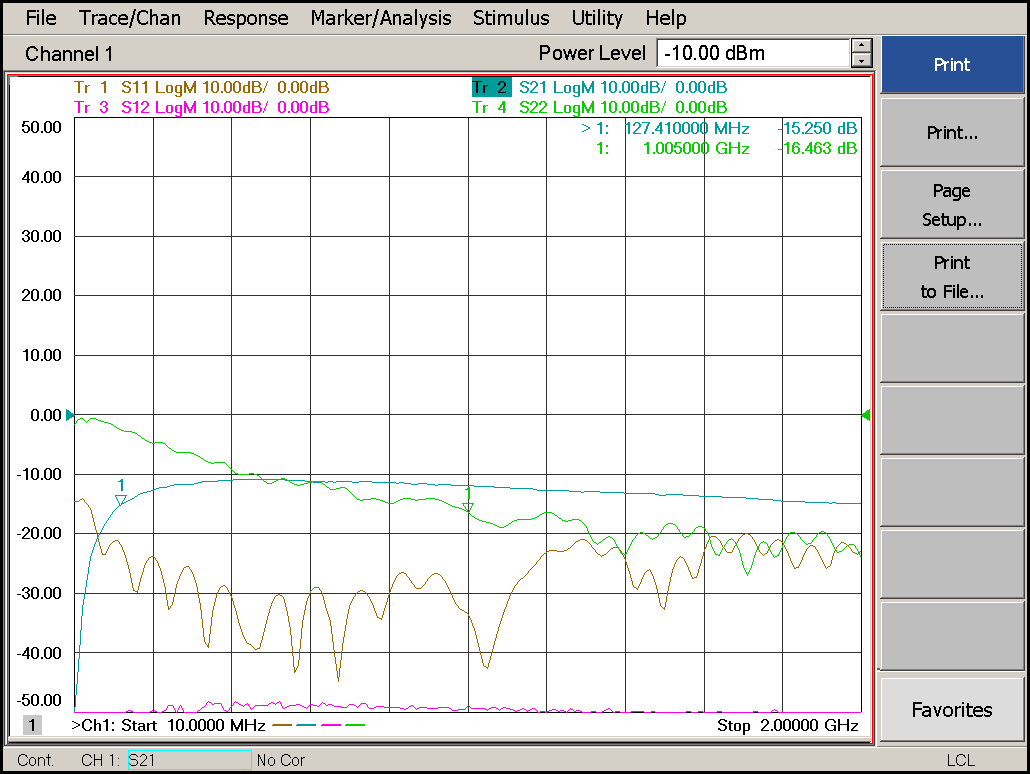
\includegraphics[width=.9\linewidth]{Documentation/figures/Correct_20_atten.png}
 \caption{Desired VNA Display for 20 Attenuation}
 \label{fig:Attenuation_20}
 \end{figure}
 
\end{enumerate}

Once completed on the first attemplifier, this process is repeated for the other fifteen. Note that the SMA cables must be moved to the next set of IN and OUT feed throughs as well as the number after the -n in the attenuation commands for each subsequent attemplifier. Refer to Table \ref{tab:Front_to_attemp} regarding which IN and OUT feed throughs connect to which attemplifier. 

\subsection{Troubleshooting}
\label{sec:8.3}
% ----------------------------------------------------------------

During testing, not all the attemplifiers had the desired results. This section will highlight problematic VNA results and their cause. Note that because this section only reflects the the problems that were experienced while testing the ATA's twenty two Attemplifier Modules, not all \emph{possible} problems that one can experience while testing are listed here.

The most common issue that was encountered was all or half of the attemplifiers not responding to commands and being stuck on one of the three incorrect graphs in Figure \ref{fig:three graphs}. This problem is caused by a short in at least one attemplifiers. If the graph displayed is Figure \ref{fig:shortout_yellow}, then the short is caused by a clock (yellow) wire. If the graph displayed is Figure \ref{fig:shortout_white}, then the short is caused by a data (white) wire. If the graph displayed is Figure \ref{fig:shortout_red}, then the short is caused by a power (red) wire. Regarding this case, only half of the attemplifiers will be effected. This is because the attemplifiers are in two circuits, so when the power is shorted on one attemplifier, it only effects the attemplifiers in the same circuit.  These shorts were most often caused by one or more wires (yellow, white, green, and/or red) being swapped with its corresponding ground (black) wire in the connector. Figure \ref{fig:pinout} shows the proper pin out of an attemplifier connector. For a reminder of the functionality of each attemplifier wire, refer to Table \ref{table: Wire_func}. Shorts also occurred, though less often, from a messy solder job where the wire is connected to the attemplifier. The malfunctioning attemplifier is most easily identified by repeatedly trying to set the attenuation of one attemplfier while unplugging each of the other attemplifiers from the board until the VNA finally shows the correct display. 

\begin{figure}[H]
 \centering
 
 \begin{subfigure}[b]{.6\linewidth}
   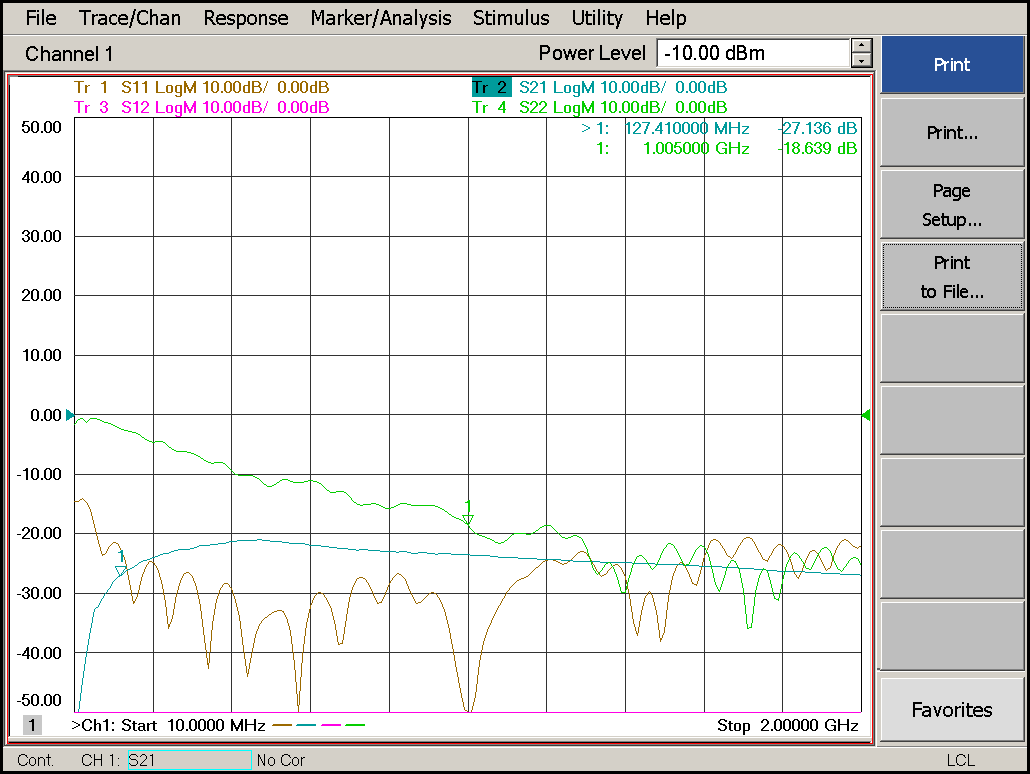
\includegraphics[width=1\linewidth]{Documentation/figures/short_yellow.png}
   \caption{}
   \label{fig:shortout_yellow}
 \end{subfigure}
 
 \begin{subfigure}[b]{.6\linewidth}
  \centering
   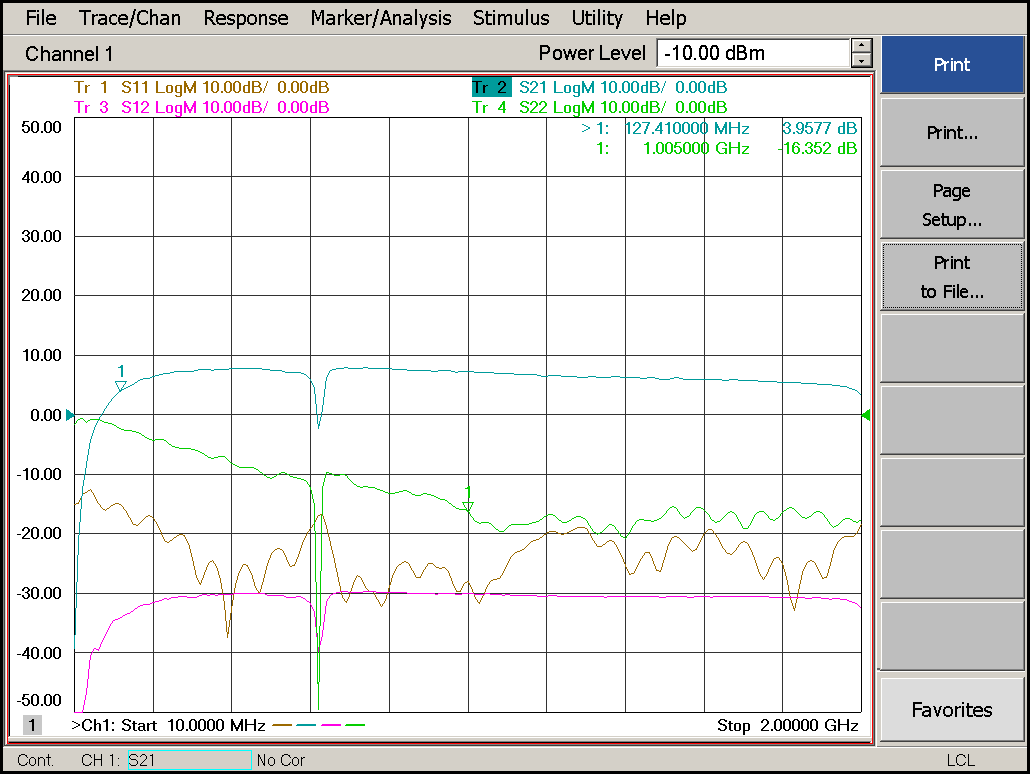
\includegraphics[width=1\linewidth]{Documentation/figures/short_white.png}
   \caption{}
   \label{fig:shortout_white}
 \end{subfigure}
 
 \begin{subfigure}[b]{.6\linewidth}
  \centering
  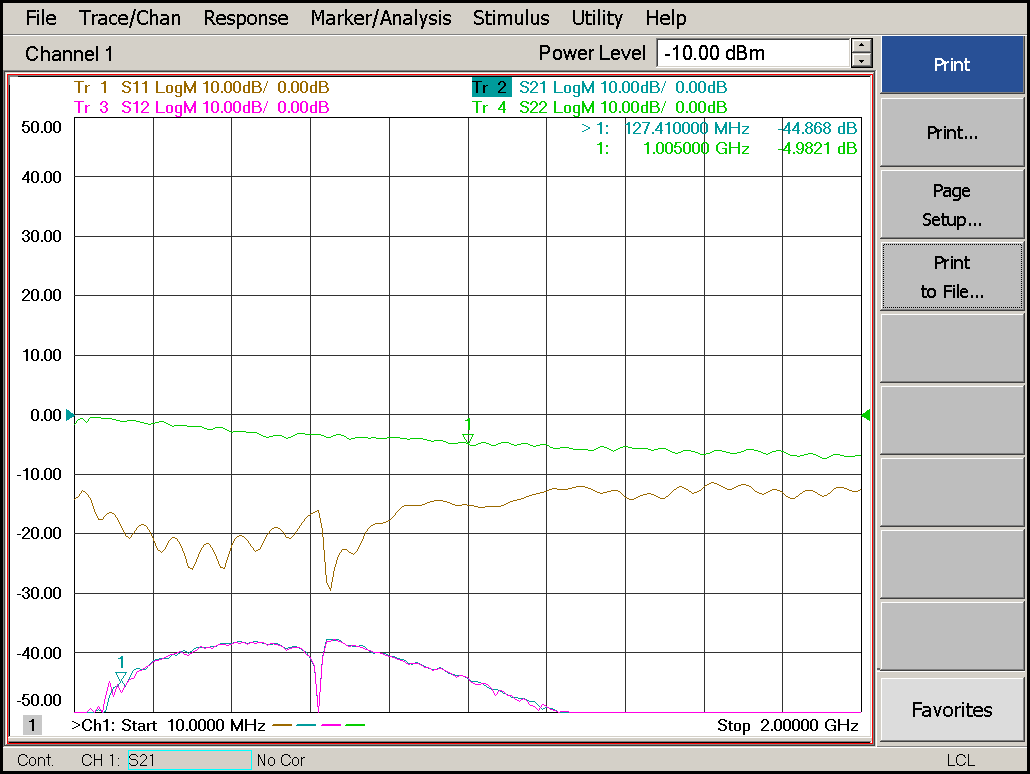
\includegraphics[width=1\linewidth]{Documentation/figures/short_power.png}
  \caption{}
  \label{fig:shortout_red}
 \end{subfigure}

 \caption{VNA Display of Different Attemplifier Wires Shorting Out}
 \label{fig:three graphs}
 
\end{figure}


Another common problem that was experienced was two neighboring attemplifier connectors being switched on the control board. This caused the first attemplifier to not respond to any command as shown in Figure \ref{fig:Before_atten}, but the second attemplifier to be set to an attenuation once the SMA cables were moved over. Thus, if this issue is suspected, leave the SMA cables attached to the first attemplifier while changing the attemplifier to the second in the command line.

An additional commonly encountered issue was a single attemplifier not responding to commands and being stuck on an incorrect graph. This problem has the most possible explanations. If the graph appears like Figure \ref{fig:shortout_yellow}, then the yellow wire is broken. If the graph appears like Figure \ref{fig:shortout_white}, then the white wire is broken. If the graph appears like Figure \ref{fig:shortout_red}, then the red wire is broken. If the graph appears like Figure \ref{fig:green_broken}, then the green wire is broken. 


 \begin{figure}[H]
 \centering
 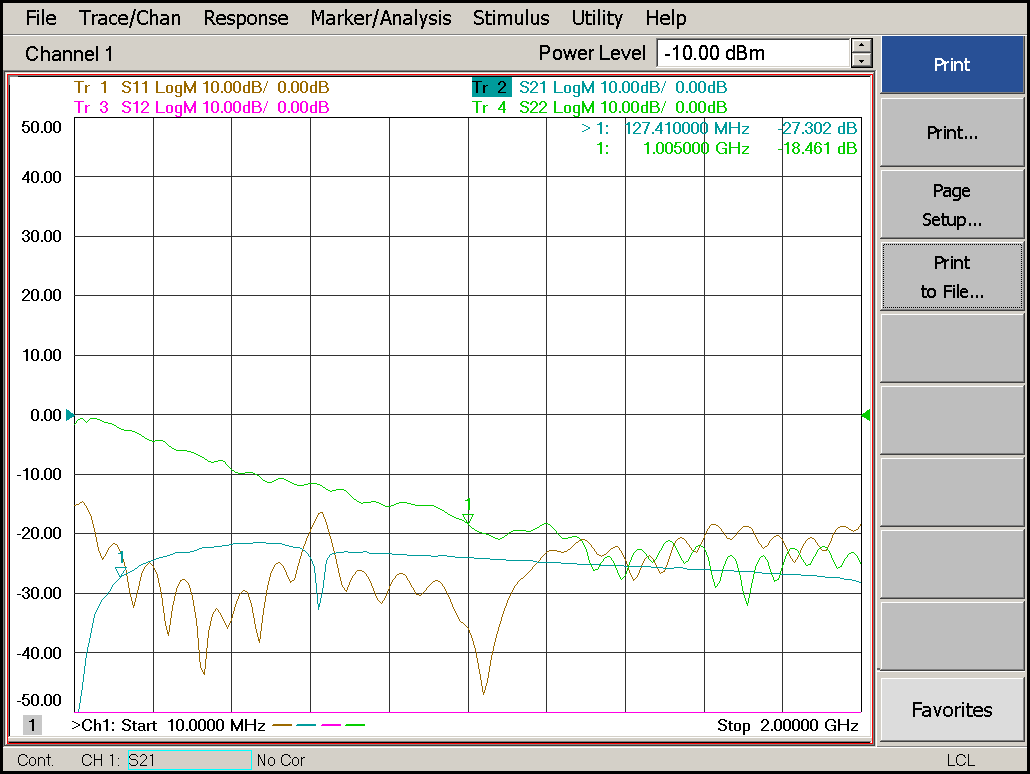
\includegraphics[width=1\linewidth]{Documentation/figures/green_broken.png}
 \caption{VNA Display when Green Wire is Broken}
 \label{fig:green_broken}
 \end{figure}
 
 Another possible cause of a single attemplifier not responding to commands is its green and corresponding ground wire being switched. If this is the case, the graph will appear as shown in Figure \ref{fig:shortout_yellow}.
 
 Finally, if none of the above are the root of the problem, the attemplifier itself may be broken. This only occurred once while testing all twenty two attemplifier modules, and the resulting graph is shown in Figure \ref{fig:broken_attemplifier}. Note that are multiple ways an attemplifier can break meaning that not all broken attemplifiers will have a graph like Figure \ref{fig:broken_attemplifier}. 
 
 \begin{figure}[H]
 \centering
 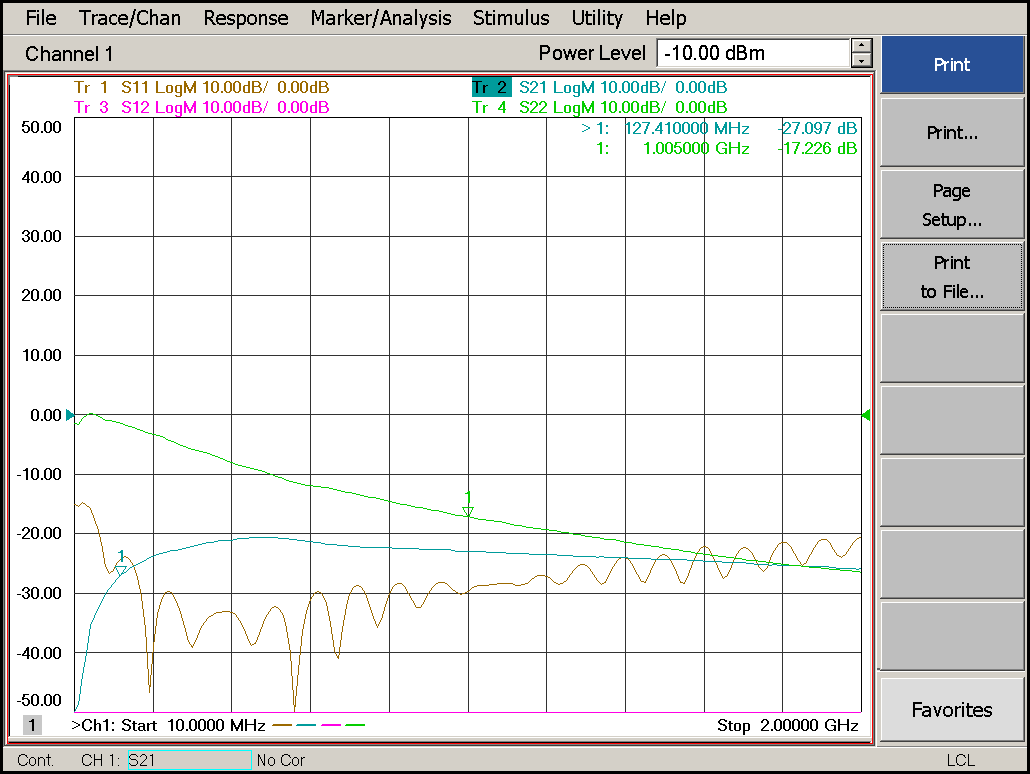
\includegraphics[width=1\linewidth]{Documentation/figures/broken_attemp.png}
 \caption{VNA Display when an Attemplifier is Broken}
 \label{fig:broken_attemplifier}
 \end{figure}
 
 Recall that all the above troubleshooting is not a complete list of all the problems that can be experienced with an Attemplifier Module. Instead, they are just the issues encountered when testing the ATA Attemplifier Modules.
 
 \newpage
 
%----------------------------------------------------------------------------------------
%	Appendix A: Attemplifier Module Enclosure Drawings
%----------------------------------------------------------------------------------------

\appendix
% ----------------------------------------------------------------


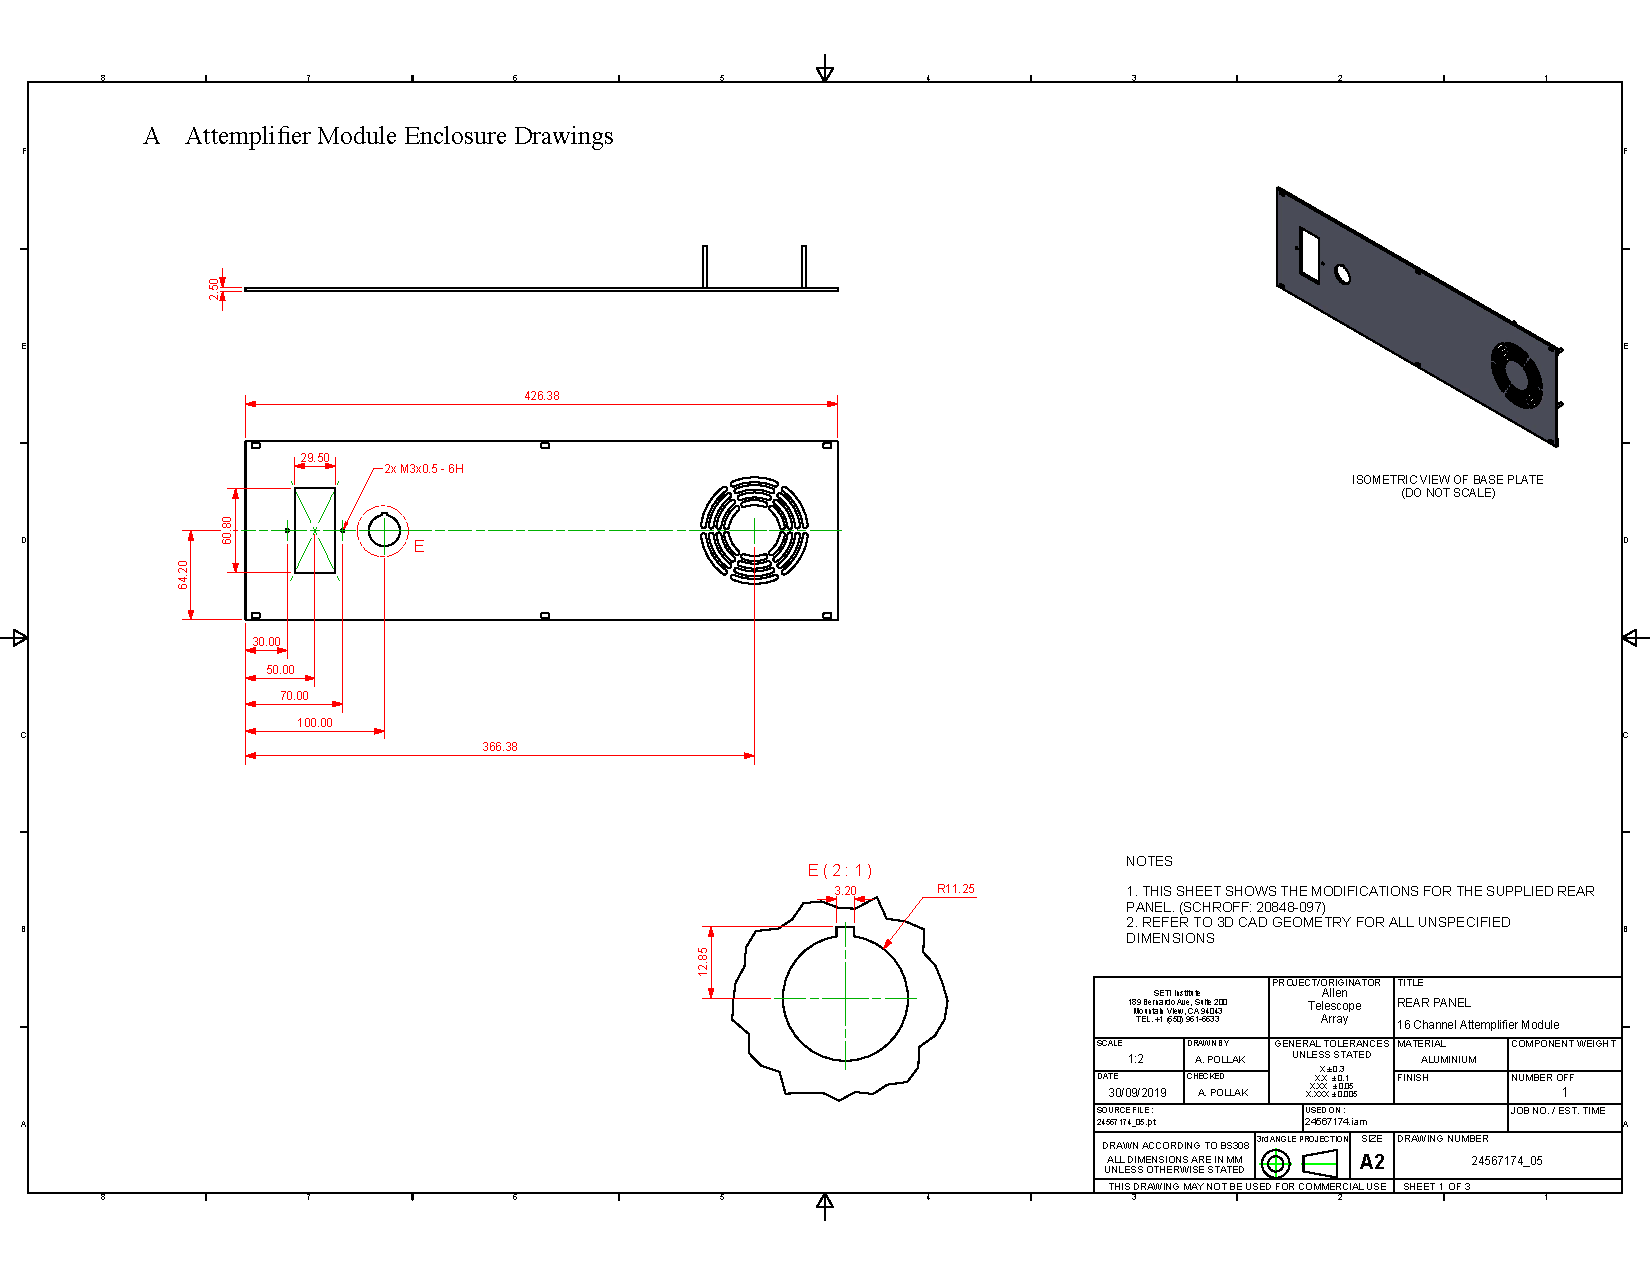
\includepdf[pages=-, landscape=true]{Documentation/PDFs/24567174_05(copy).pdf}
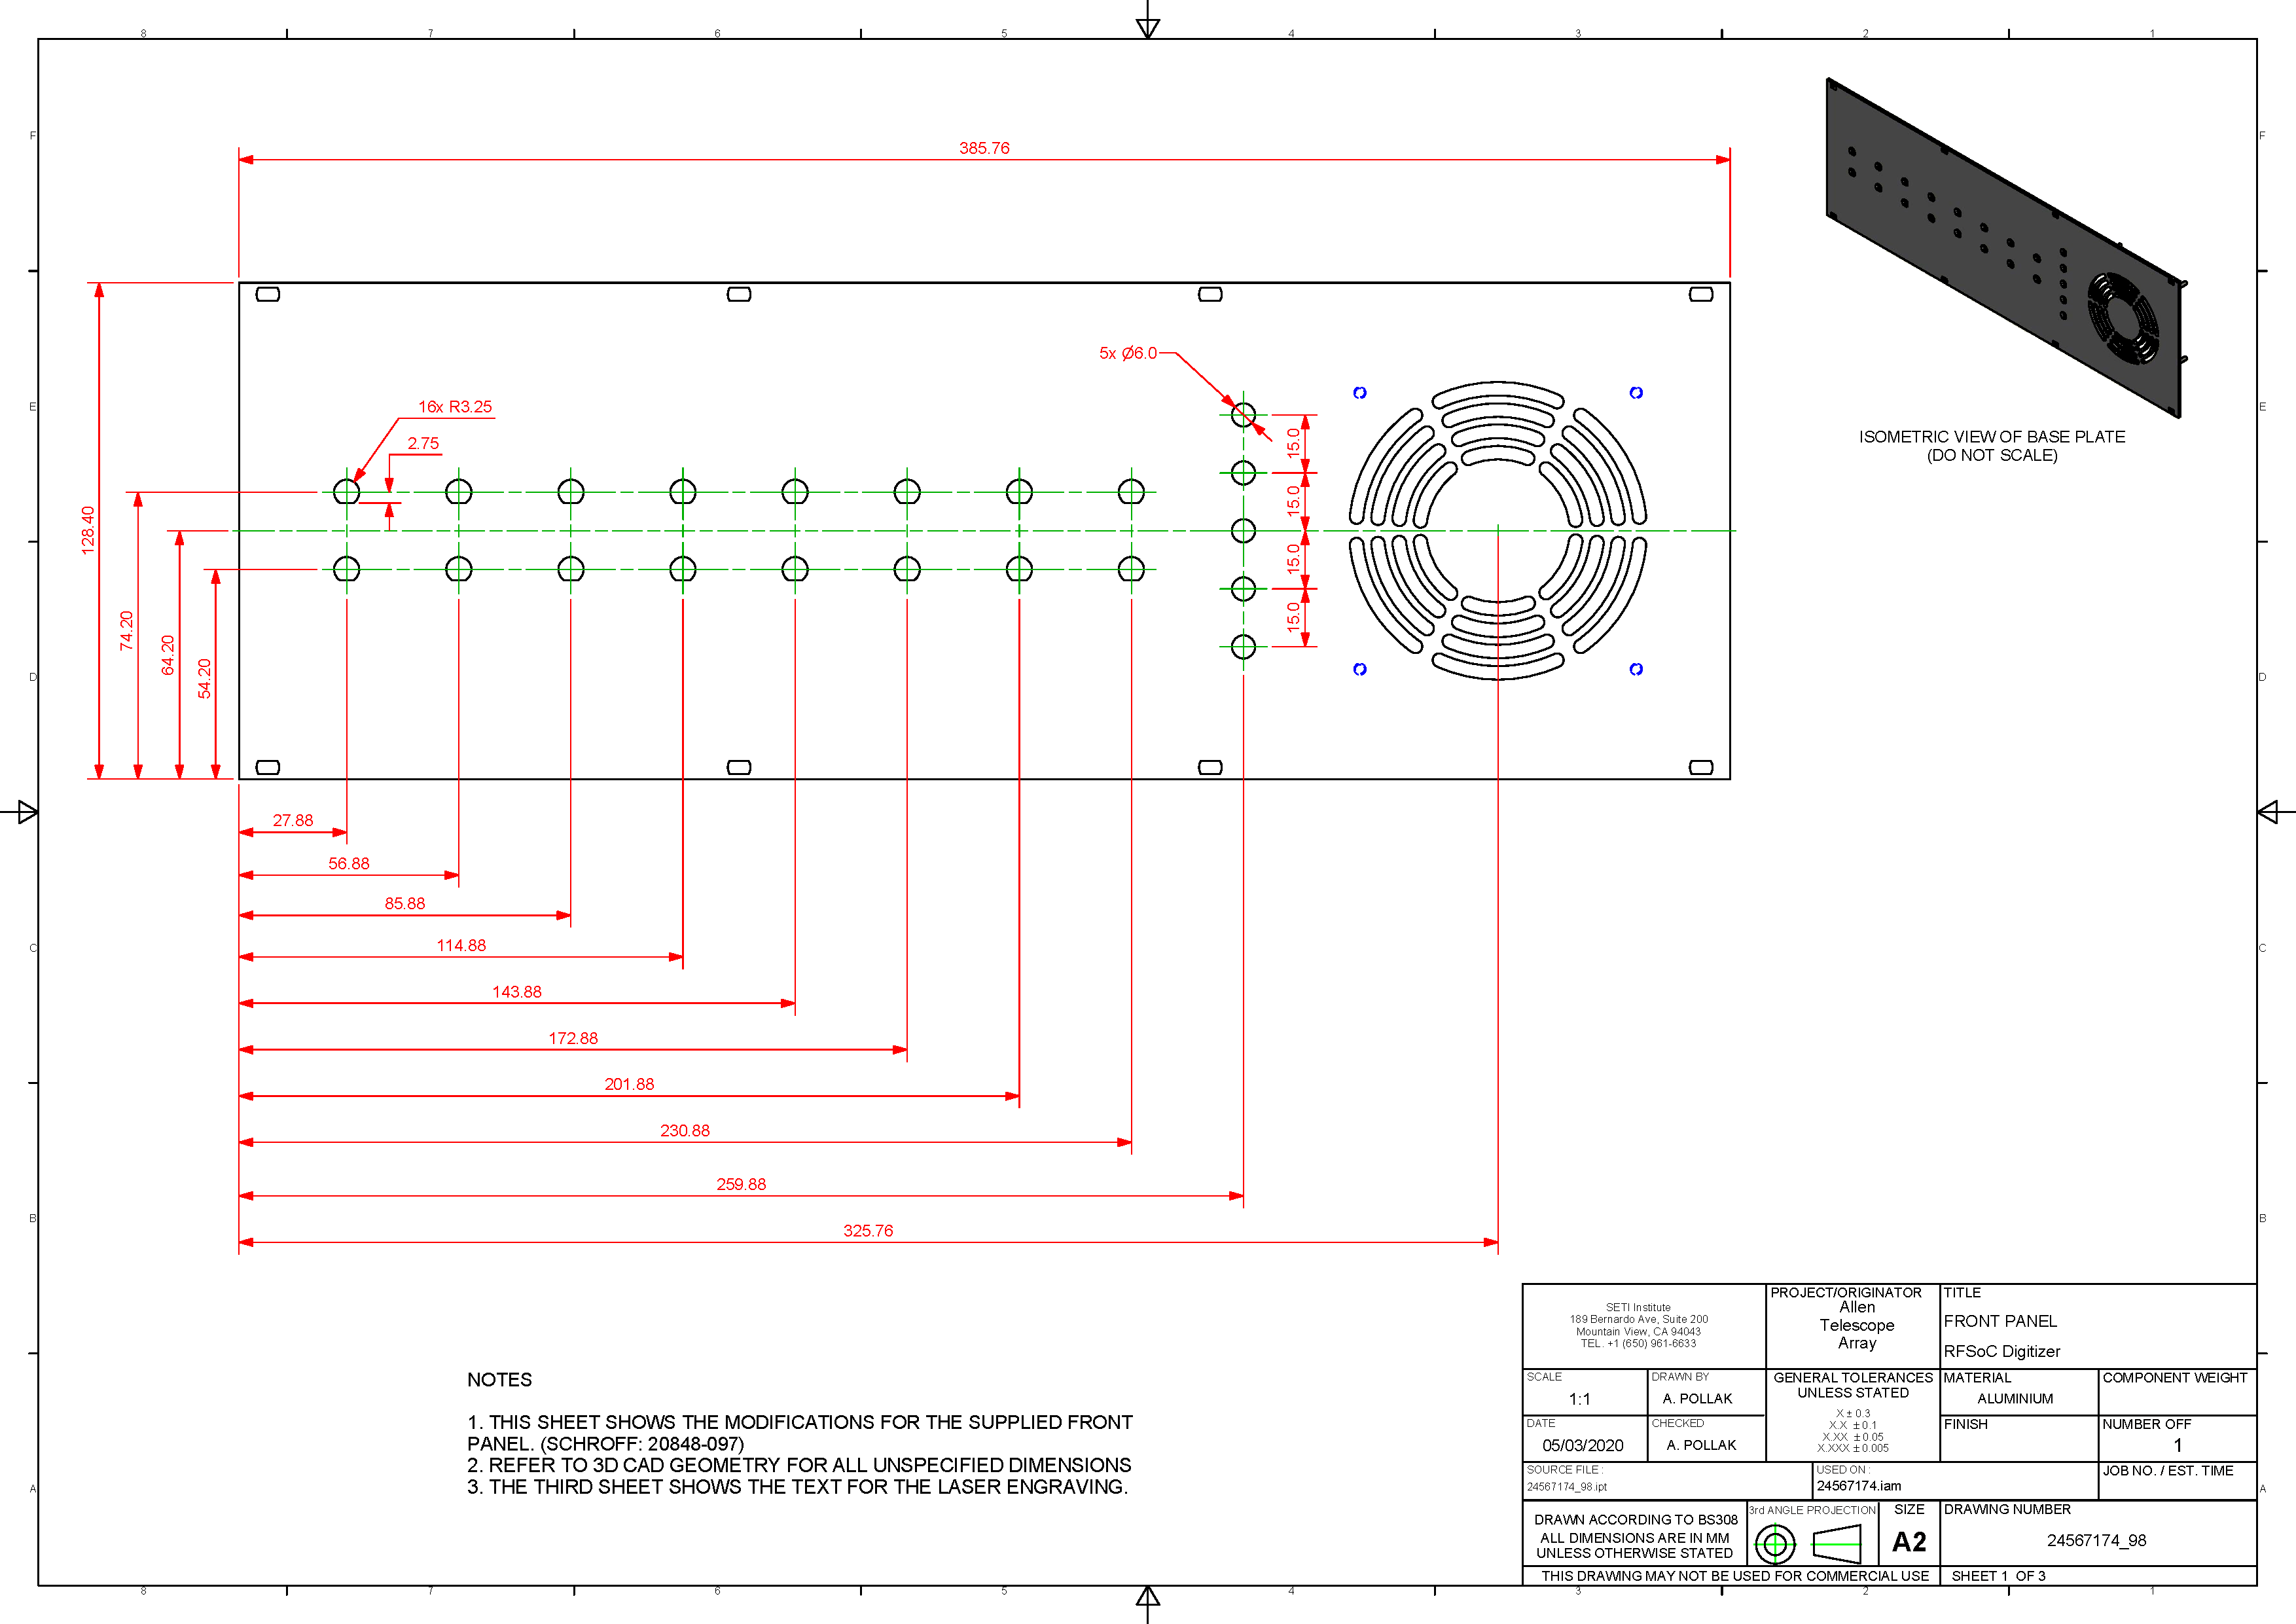
\includepdf[pages=-, landscape=true]{Documentation/PDFs/24567174_98.pdf}
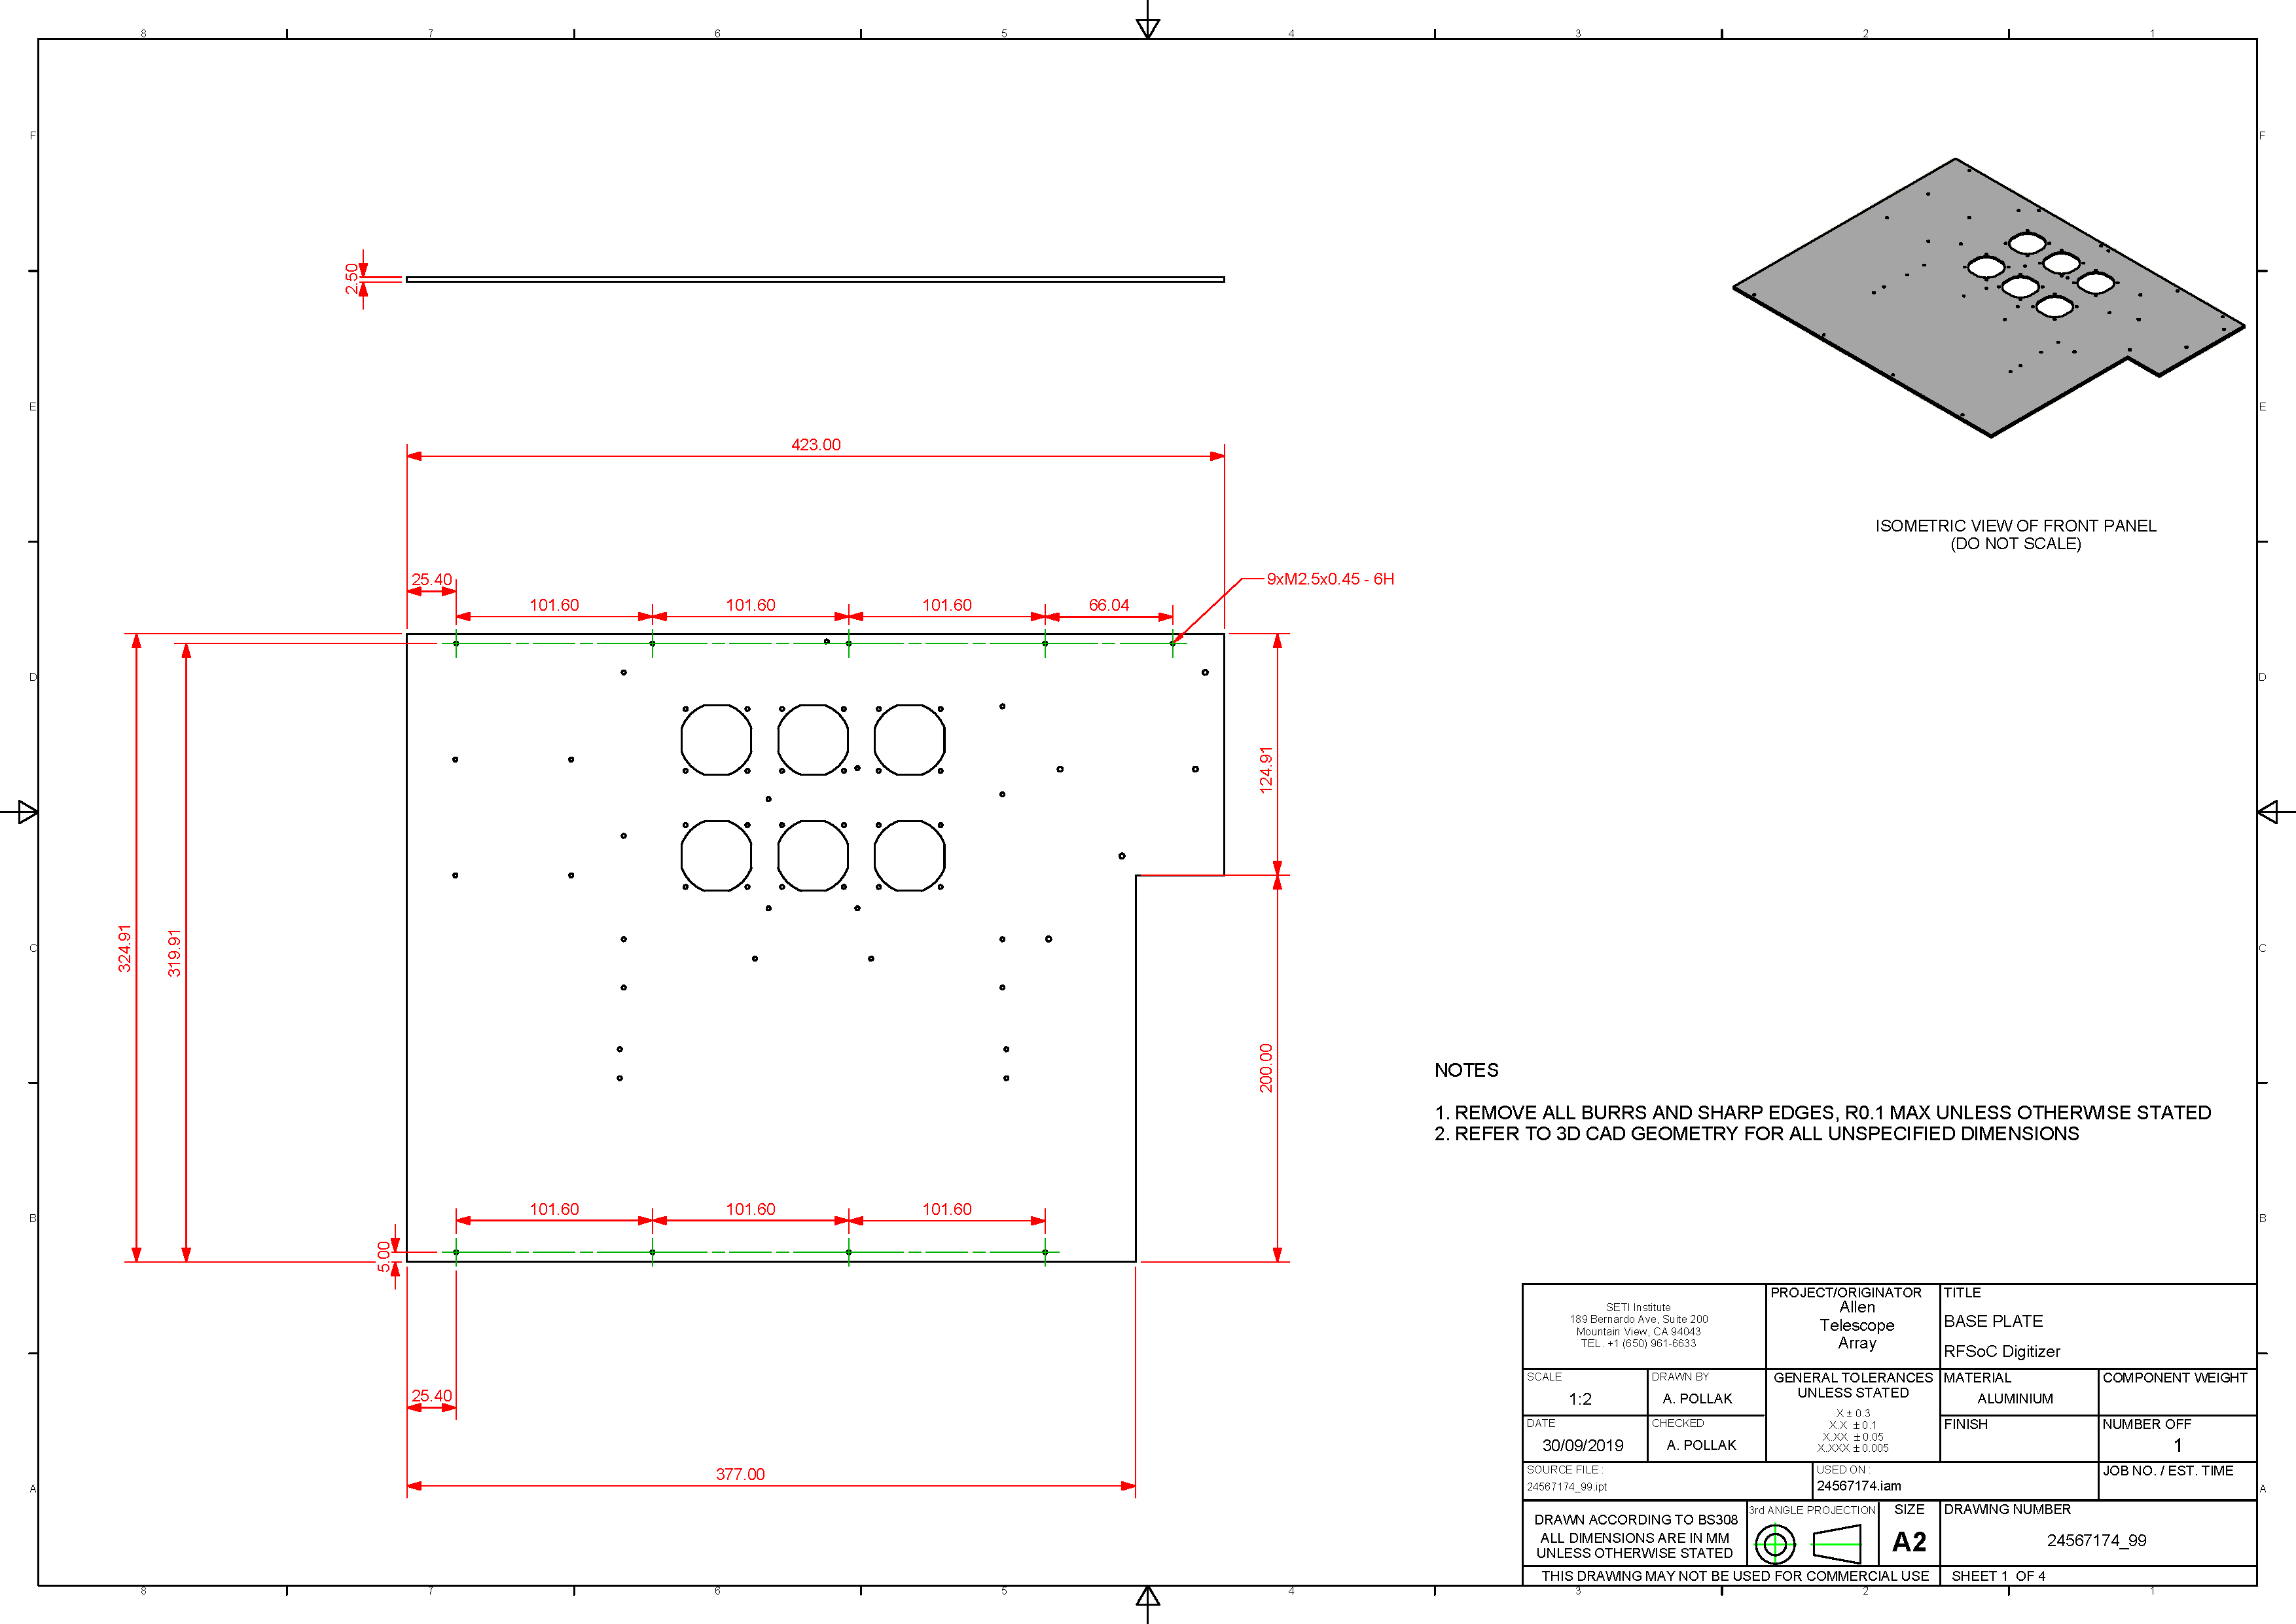
\includepdf[pages=-, landscape=true]{Documentation/PDFs/24567174_99.pdf}
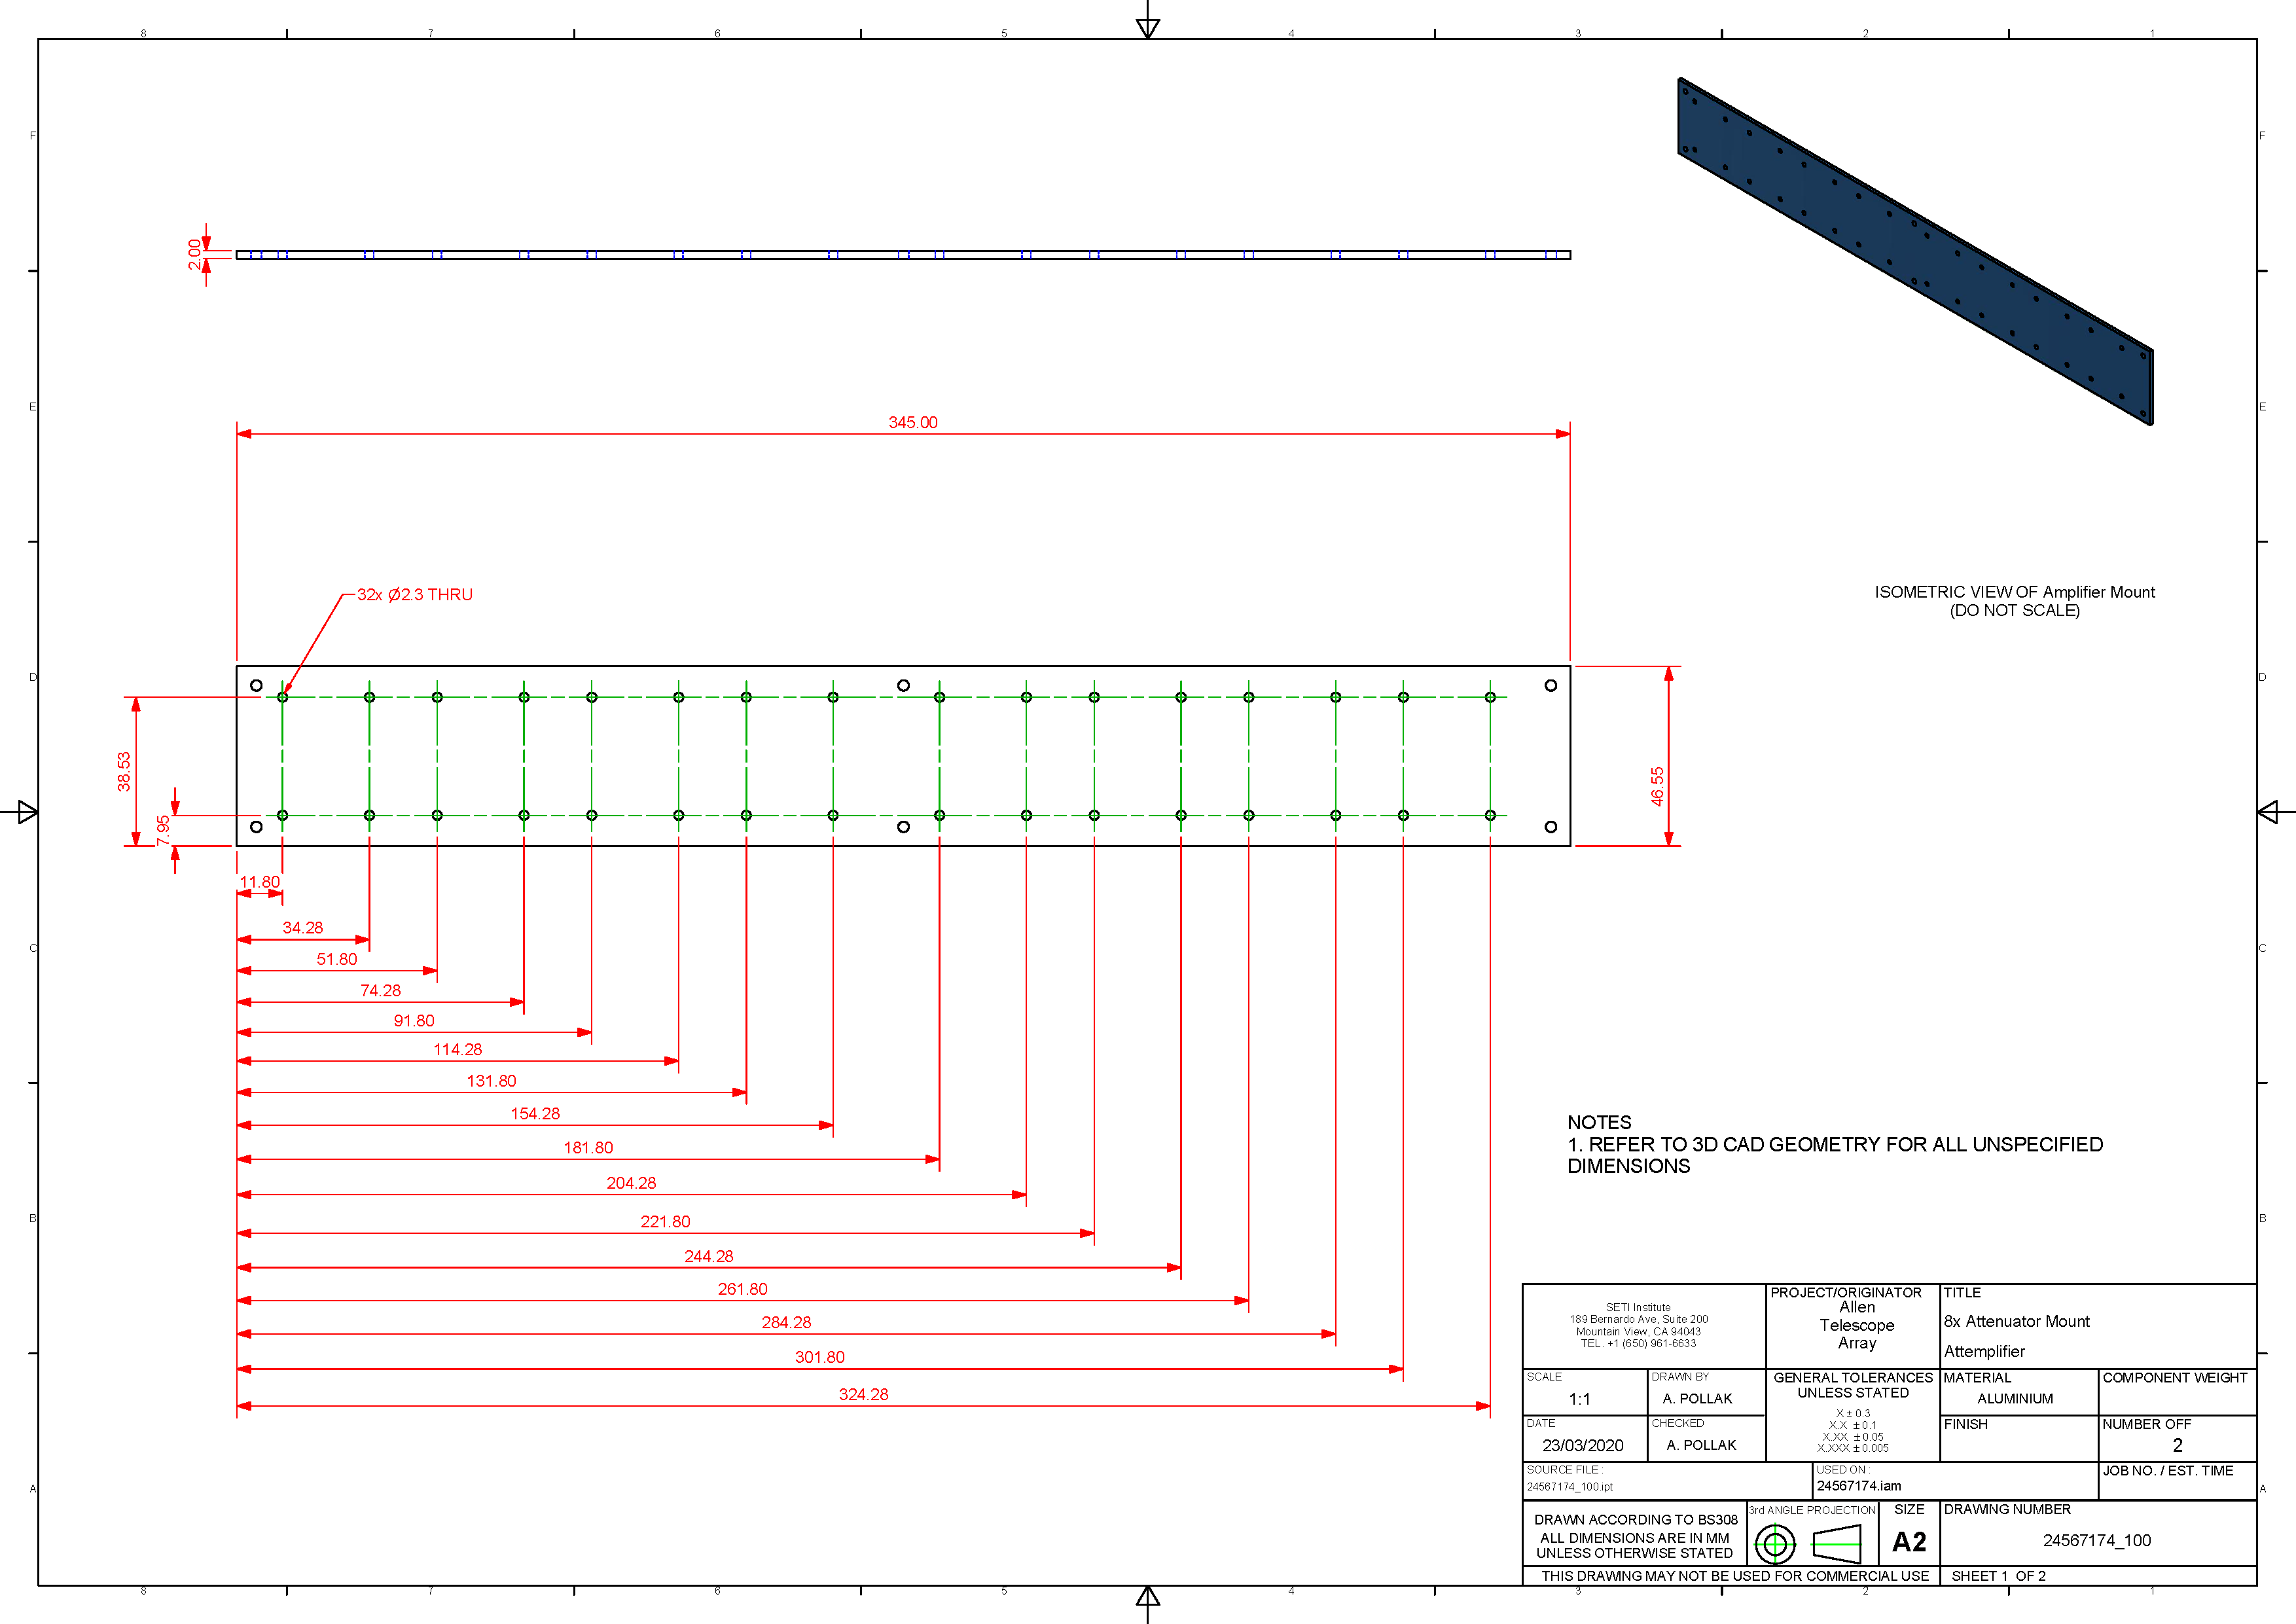
\includepdf[pages=-, landscape=true]{Documentation/PDFs/24567174_100.pdf}

%----------------------------------------------------------------------------------------
%	Appendix B: Attemplifier Module Component List
%----------------------------------------------------------------------------------------
\begin{landscape}
\section*{B \hspace{.5cm} Component List of Attemplifier Module}

% ----------------------------------------------------------------

\begin{table}[H]
\centering
\resizebox{1.5\textwidth}{!}{%
\begin{tabular}{@{}lllllll@{}}
\toprule
Qty & Unit & Description & Manufacturer & PN Manufacturer & Distributor & PN Distributor\\
\midrule
1 & Each & EuropacPRO kit, heavy design, shielded, with front handles & Schroff & 
24563-174 \\
1 & Each & Linear regulators, single 12V 4.2A & Schroff & 13105-012\\
1 & Each & Front Panel PSG 14 HP 19" AC/DC Linear & Schroff & 21005-474\\
1 & Each & Connector H 15 F, FASTON connection & Schroff & 69001-733\\
1 & Pack & Enclosure Accessory, Grey, Plastic Sleeve & Schroff & 21100-464 & Newark & 74M6491\\
1 & Pack & 21101-101 -  COLLAR SCREW, PK100 & Schroff & 21101-101 & Newark & 74M6493\\
1 & Each & Front Panel & Front Panel Express, LLC & ATA-AP-24567174\_98.fpd\\
1 & Each & Rear Panel & Front Panel Express, LLC & ATA-AP-24567174\_05.fpd\\
1 & Each & Base Plate & Front Panel Express, LLC & ATA-AP-24567174\_99.fpd\\
2 & Each & Attemplifier Mount & Front Panel Express, LLC & ATA-AP-24567174\_100.fpd\\
1 & Each & USB 2.0 connection cable, USB B male Micro B, open end & Amazon\\
1 & Each & 40p to 40p GPIO Ribbon Cable for Raspberry Pi 4/3 / Zero / 2 (8" 20cm) & Amazon\\
1 & Each & 1ft (0.3m) Cat6 Snagless Unshielded (UTP) PVC CM Ethernet Network Patch Cable, Blue & FS & C6-UTPSGPVCBE-0.3M\\
1 & Each & 4304.4005 -  INLET FILTER, IEC, C14, FKH, 10A & Schurter & 43,044,005 & Newark & 83T7492\\
1 & Each & Modular Connector, RJ45 Plug & Schneider Electric & XB5PRJ45 & Newark & 49AC2992\\
1 & Each & RPI2-MODB-V1.2 & RASPBERRY-PI & RPI2-MODB-V1.2 & Newark & 95Y1948\\
1 & Each & MEAN WELL RS-15-5 AC to DC Power Supply Single Output, 5V 3 Amp 15W & Mean Well & RS-15-5 & Newark & 44AC7311\\
1 & Pack & Machine Screw, M2, 6mm & TR FASTENINGS & M26 CSSTMCZ100- & Newark & 53M8644\\
1 & Pack & Socket Screw, M3, 16mm & TR FASTENINGS & M3 16 SO12CS S100 & Newark & 53M8745\\
1 & Pack & Socket Screw, M3, 10mm & TR FASTENINGS & M3 10 SO12CS S100 & Newark & 53M8712\\
1 & Pack & Machine Screw, M2.5, 5mm & TR FASTENINGS & 173-202579H & Newark & 25M0782\\
1 & Pack & Machine Screw, M3, 6 mm & TR FASTENINGS & M3 6 KRSTMC Z100 & Newark & 53M8781\\
1 & Pack & Machine Screw, M2.5, 10 mm & TR FASTENINGS & M2.510 CSSTMCZ100- & Newark & 53M8599\\
1 & Pack & Machine Screw, M3, 16 mm & TR FASTENINGS & M316 KSSTMCZ100- & Newark & 53M8739\\
1 & Each & Modular Connector, RJ45 Plug & SCHNEIDER ELECTRIC & XB5PRJ45 & Newark & 49AC2992\\
6 & Each & Terminal, Locking, CLS Series, 22AWG to 18AWG, M3.5, \#6 & MULTICOMP & CLS-TV-1806 & Newark & 14T2409\\
1 & Each & Fuse, Cartridge, Slow Blow, 1 A, 250 V & Littlefuse & 0217001.HXP & Newark & 26K8001\\
1 & Pack & Guide Rail, Red, 160mm, 10 Pieces, Plug‐in and Frame Type Units, EuropacPRO Series & Schroff & 24560-351 & Newark & 44W8824\\
1 & Pack & Quick Disconnect Terminal, FDFD1 Series & MULTICOMP PRO & FDFD1-250 & Newark & 89K2088\\
1 & Pack & Quick Disconnect Terminal,PBDD2 Series, Female Piggyback Disconnect, 6.35mm x 0.81mm & MULTICOMP PRO & PBDD2-250 & Newark & 89K2146\\
1 & Each & DC Fans DC Fan, High Airflow Series, 80x80 & Sunon & PF80251V1-1000U-A99 & Mouser & 369-PF80251V11UA99\\
2 & Each & LED Panel Mount Indicator, Blue, 3.8 VDC, 6 mm, 20 mA & APEM & Q6F7BXXB02E & Mouser & 642-Q6F7BXXB02E\\
3 & Each & LED Panel Mount Indicator, Yellow, 2.0 VDC, 6 mm, 20 mA & APEM & Q6F3GXXY02E & Mouser & 642-Q6F3GXXY02E\\
3 & Each & LED Panel Mount Indicator, Green, 2.0 VDC, 6 mm, 20 mA & APEM & Q6F1CXXG24E & Mouser & 642-Q6F1CXXG24E\\
12 & Each & STANDOFF, HEX MALE-FEMALE, 25MM, M2.5 & RAF & M2120-2545-AL & Mouser & 761-M2120-2545-AL\\
8 & Each & STANDOFF, HEX MALE-FEMALE, 10MM, M2 & Wurth Elektronik & 971100244 & Mouser & 710-971100244\\
20 & Each & Headers \& Wire Housings 2 PIN SIL HOUSING & Harwin & M20-1060200 & Mouser & 855-M20-1060200\\
16 & Each & SMA Male to SMA Female Bulkhead Semi-Flexible Precision Cable 12 Inch Length Using PE-SR405FLJ Coax, LF Solder, RoHS & Pasternack & PE39433-12 & Pasternack & PE39433-12\\
16 & Each & SMA Male to SMA Female Bulkhead Semi-Flexible Precision Cable 9 Inch Length Using PE-SR405FLJ Coax, LF Solder, RoHS & Pasternack & PE39433-9 & Pasternack & PE39433-9\\
16 & Each & SMA Female to SMA Female Adapter & Pasternack & PE9070 & Pasternack & PE9070\\

\bottomrule            
\end{tabular}}
\label{tab:Attemp_components}
\end{table}

\newpage

%----------------------------------------------------------------------------------------
%	Appendix C: Control Board Component List
%----------------------------------------------------------------------------------------

\section*{C \hspace{.5cm} Control Board Component List}

% ----------------------------------------------------------------

\begin{table}[H]
\centering
\resizebox{1.5\textwidth}{!}{%
\begin{tabular}{@{}lllllll@{}}
\toprule
Qty & Unit & Description & Manufacturer & PN Manufacturer & Distributor & PN Distributor\\
\midrule

1 & Each & Attemplifier Module Control Board & AP\\
1 & Each & PCB V2.0 & AP\\
1 & Each & Littelfuse 1A T Non-Resettable Surface Mount Fuse, 125 V & Littlefuse & 0154001.DRT & Newark & 98K4354\\ 
1 & Each & Fuse, Surface Mount, 1.5 A, NANO 452 Series, 125 VAC, 32 VDC, Time Delay, SMD & Littlefuse & 045201.5MRL & Newark & 12J2905\\
1 & Each & Electrolytic Capacitor, 220 µF, 35 V, M Series, ± 20\%, Radial Leaded, 8 mm & Panasonic & ECA-1VM221 & Newark & 96K9201\\
1 & Each & Surface Mount Tantalum Capacitor, 100 µF, 25 V, 2917 [7343 Metric], T491 Series, ± 10\%, -55 °C & Kemet & T491X107K025AT & Newark & 89W0515\\
3 & Each & KEMET C0805C224K1RACTU 220nF Multilayer Ceramic Capacitor MLCC 100V dc ±10\% Tolerance SMD & Kemet & C0805C224K1RACTU & Newark & 70R0966\\
3 & Each & KEMET C0805C104K5RACTU 100nF Multilayer Ceramic Capacitor MLCC 50V dc ±10\% Tolerance SMD & Kemet & C0805C104K5RACTU & Newark & 19C6015\\
1 & Each & DECODER/DEMULTIPLEXER, 4:16 & NEXPERIA & 74HC154PW,118 & Newark & 72Y1235\\
2 & Each & LM340AT-5.0/NOPB Linear Voltage Regulator, 2.4A 5 V, ±2\%, 3-pin TO-220 &  Texas Instruments & LM340AT-5.0/NOPB & Newark & 28AH3328\\
1 & Each & Inverter, Schmitt Trigger, MC14584, 1 Input, 8.8 mA, 3 V to 18 V, SOIC-14 & ON SEMICONDUCTOR & MC14584BDG & Newark & 45J1140\\
1 & Each &  LINEAR VOLT REG, 5V, 1.5A, TO-263-3 & Texas Instruments & LM340SX-5.0/NOPB & Newark & 33AH4171\\
4 & Each & LED, QuasarBrite, Green, SMD, 1206, 20 mA, 2.2 V, 565 nm & LUMEX & SML-LX1206GW-TR & Newark & 77K7035\\
3 & Each & LED, QuasarBrite, Yellow, SMD, 1206, 20 mA, 2 V, 590 nm & LUMEX & SML-LX1206SYC-TR & Newark & 75K1450\\
8 & Each & 0805 [2012 Metric], 200 ohm, ERJP06 Series, 400 V, Thick Film, 500 mW & Panasonic & ERJ-6ENF2000V & Newark & 65T8714\\
17 & Each & 0805 [2012 Metric], 150 ohm, ERJP06 Series, 400 V, Thick Film, 500 mW & Panasonic & ERJ-P06J151V & Newark & 53W3980\\
2 & Each & Optocoupler, Transistor Output, 4 Channel, DIP, 16 Pins, 60 mA, 5.3 kV, 100 \% & VISHAY & ILQ2 & Newark & 59K0212\\
8 & Each & $4.7k\Omega$ ERA Series Metal Film Thin Film Surface Mount Fixed Resistor 0805 Case  ±0.1\% 0.125W ±25ppm/°C & Panasonic & ERA6AEB472V & Newark & 62W9080\\
2 & Each & TO220 extruded heat sink,17.9degC/W & RS & 263-251 & RS-Components & 263-251\\
1 & Each & 2.54mm CGrid Hdr Shrd /Slt .38AuLF 40Ckt & Molex & 70246-4001 & Newark & 80AH0697\\
16 & Each & Wire-To-Board Connector, 2 mm, 10 Contacts, Header, DF11 Series, Through Hole, 2 Rows & HIROSE(HRS) & DF11-10DP-2DSA(24) & Newark & 49P5014\\
16 & Each & Wire-To-Board Connector, 2 mm, 10 Contacts, Receptacle, DF11 Series, Crimp, 2 Rows & HIROSE(HRS) & DF11-10DS-2C & Newark & 49P5015\\
136 & Each & Contact, DF11 Series, Socket, Crimp, 24 AWG, Tin Plated Contacts, DF11 Socket Housings & HIROSE(HRS) & DF11-2428SC & Newark & 49P5045\\
1 & Each & Crimp Tool, Hand, Hirose DF11-2428SC, DF11-2428SCA \& DF11A-2428SC Socket Contacts, DF11 Series & HIROSE(HRS) & DF11-TA2428HC & Newark & 49P5012\\
1 & Each &  COMBICON MCV, 3.81mm Pitch, 2 Way, 1 Row, Straight PCB Terminal Block Header & Phoenix Contact & 1803426 & Newark & 71C4212\\
1 & Each & 2 way cable mount screw terminal,3.81mm & Phoenix Contact & 1803578 & Newark & 71C4221\\
1 & Each & Thermal Insulator, Insulating Kit, TO-220, Silicone Rubber, 1.6 W/m.K, 6 kV, 0.23 mm, 10 ohm-cm & MULTICOMP & MK3306/TG & Newark & 45P5588\\
1 & Each & SCREW SOCKET, CAP, S/S, A2, M3X8 & TR FASTENINGS & M38 SOA2CSS50- & Newark & 53M8805\\
5 & Each & 2.54mm Pitch 2 Way 1 Row Straight PCB Header, Solder Termination & Molex & 22-28-4023  & Newark & 92C2171\\
1 & Each & Crimpers / Crimping Tools 2.54mm HAND CRIMP TOOL & Harwin & Z20-320 & Mouser & 855-Z20-320\\
10 & Each & Headers Wire Housings F/M CRIMP TERM GOLD/TIN & Harwin & M20-1180042 & Mouser & 855-M20-1180042\\



\bottomrule            
\end{tabular}}
\label{tab:Attemp_components}
\end{table}

\newpage

%----------------------------------------------------------------------------------------
%	Appendix D: Control Board Schematics
%----------------------------------------------------------------------------------------

\section*{D \hspace{.5cm} Control Board Schematics}

% ----------------------------------------------------------------

%
\begin{figure}[H]
\centering
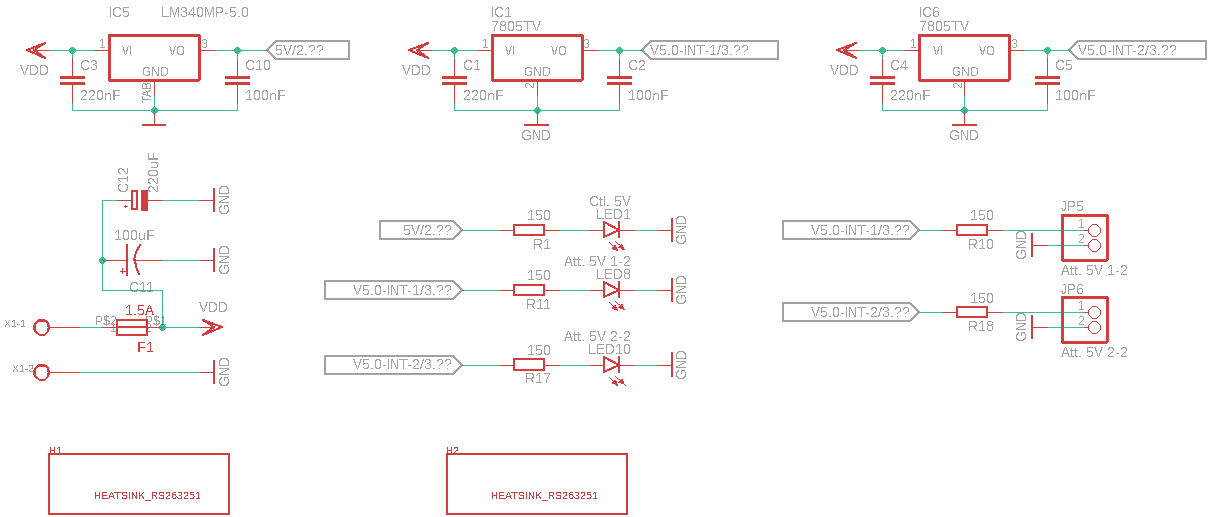
\includegraphics[width=1\linewidth]{Documentation/figures/control_board_schematic_1.png}
\caption{Control Board Schematic Part 1}
\label{fig:control_sch1}
\end{figure}
%

\end{landscape}

%
\begin{figure}[H]
\centering
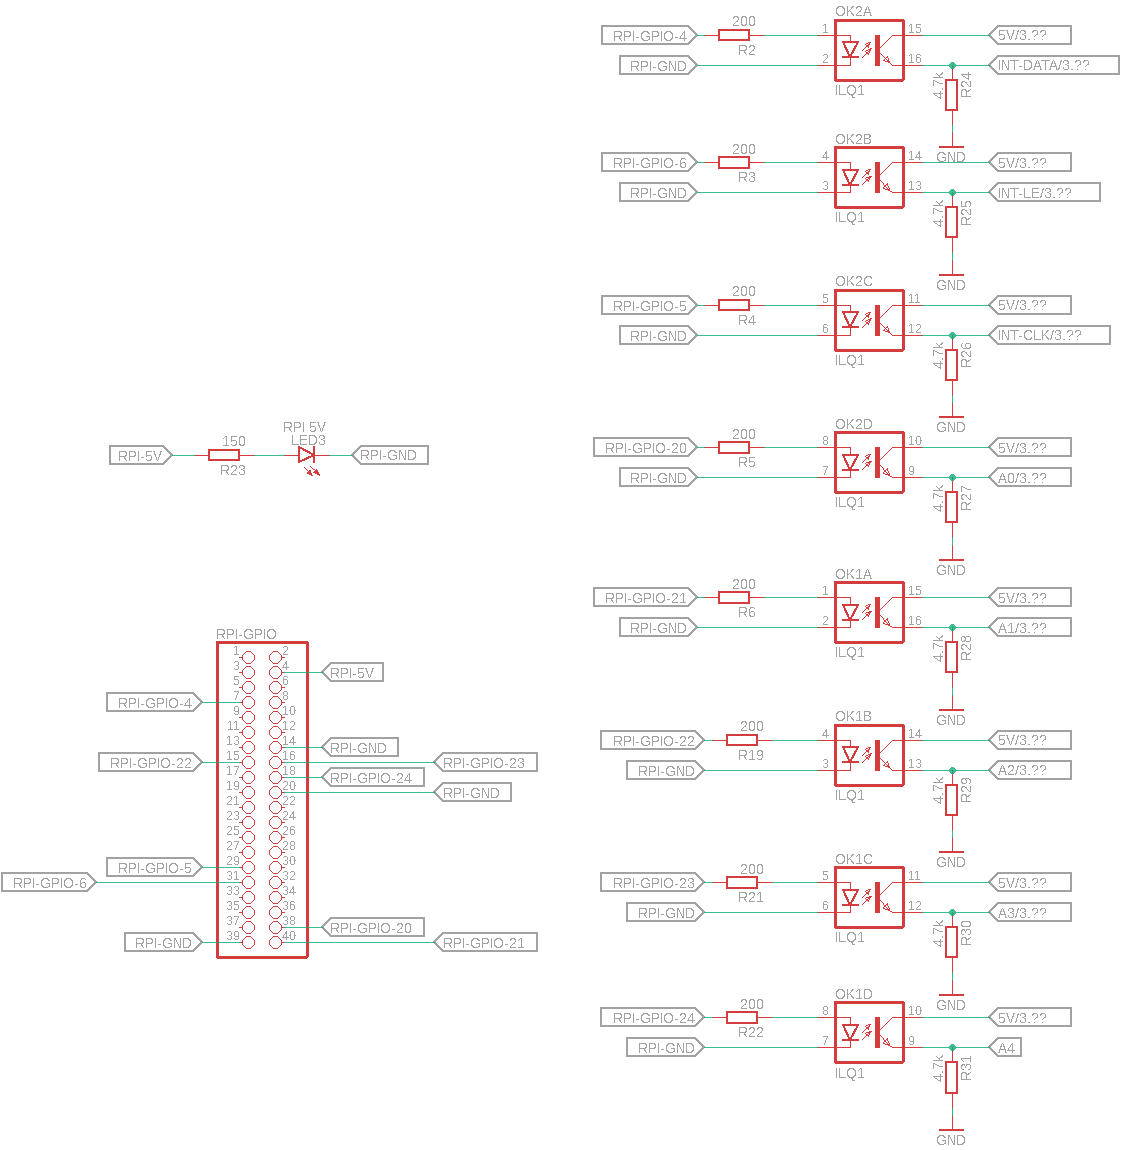
\includegraphics[width=1\linewidth]{Documentation/figures/control_board_schematic_2.png}
\caption{Control Board Schematic Part 2}
\label{fig:control_sch2}
\end{figure}
%

%
\begin{figure}[H]
\centering
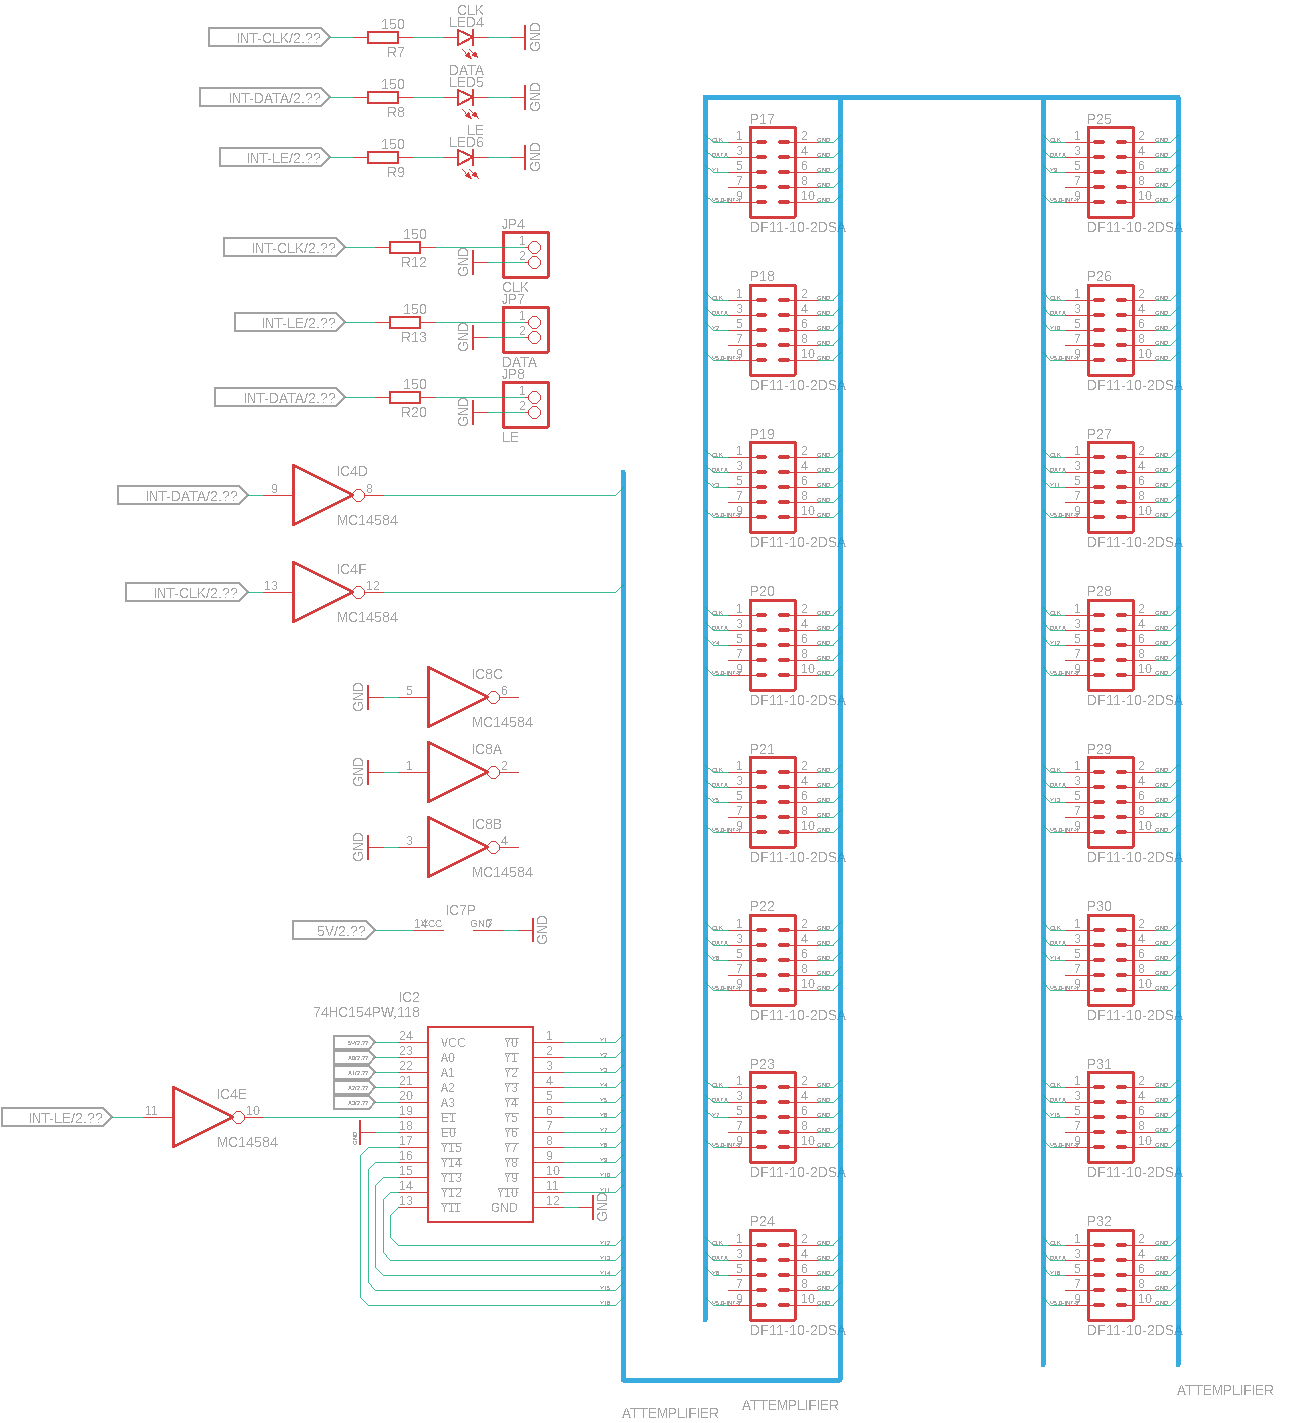
\includegraphics[width=1\linewidth]{Documentation/figures/control_board_schematic_3.png}
\caption{Control Board Schematic Part 3}
\label{fig:control_sch3}
\end{figure}
%

%----------------------------------------------------------------------------------------
%	Appendix E: Attemplifier Enclosure Drawings
%----------------------------------------------------------------------------------------
\begin{landscape}
\section*{E \hspace{.5cm} Attemplifier Enclosure Drawings}

% ----------------------------------------------------------------

 \begin{figure}[H]
 \centering
 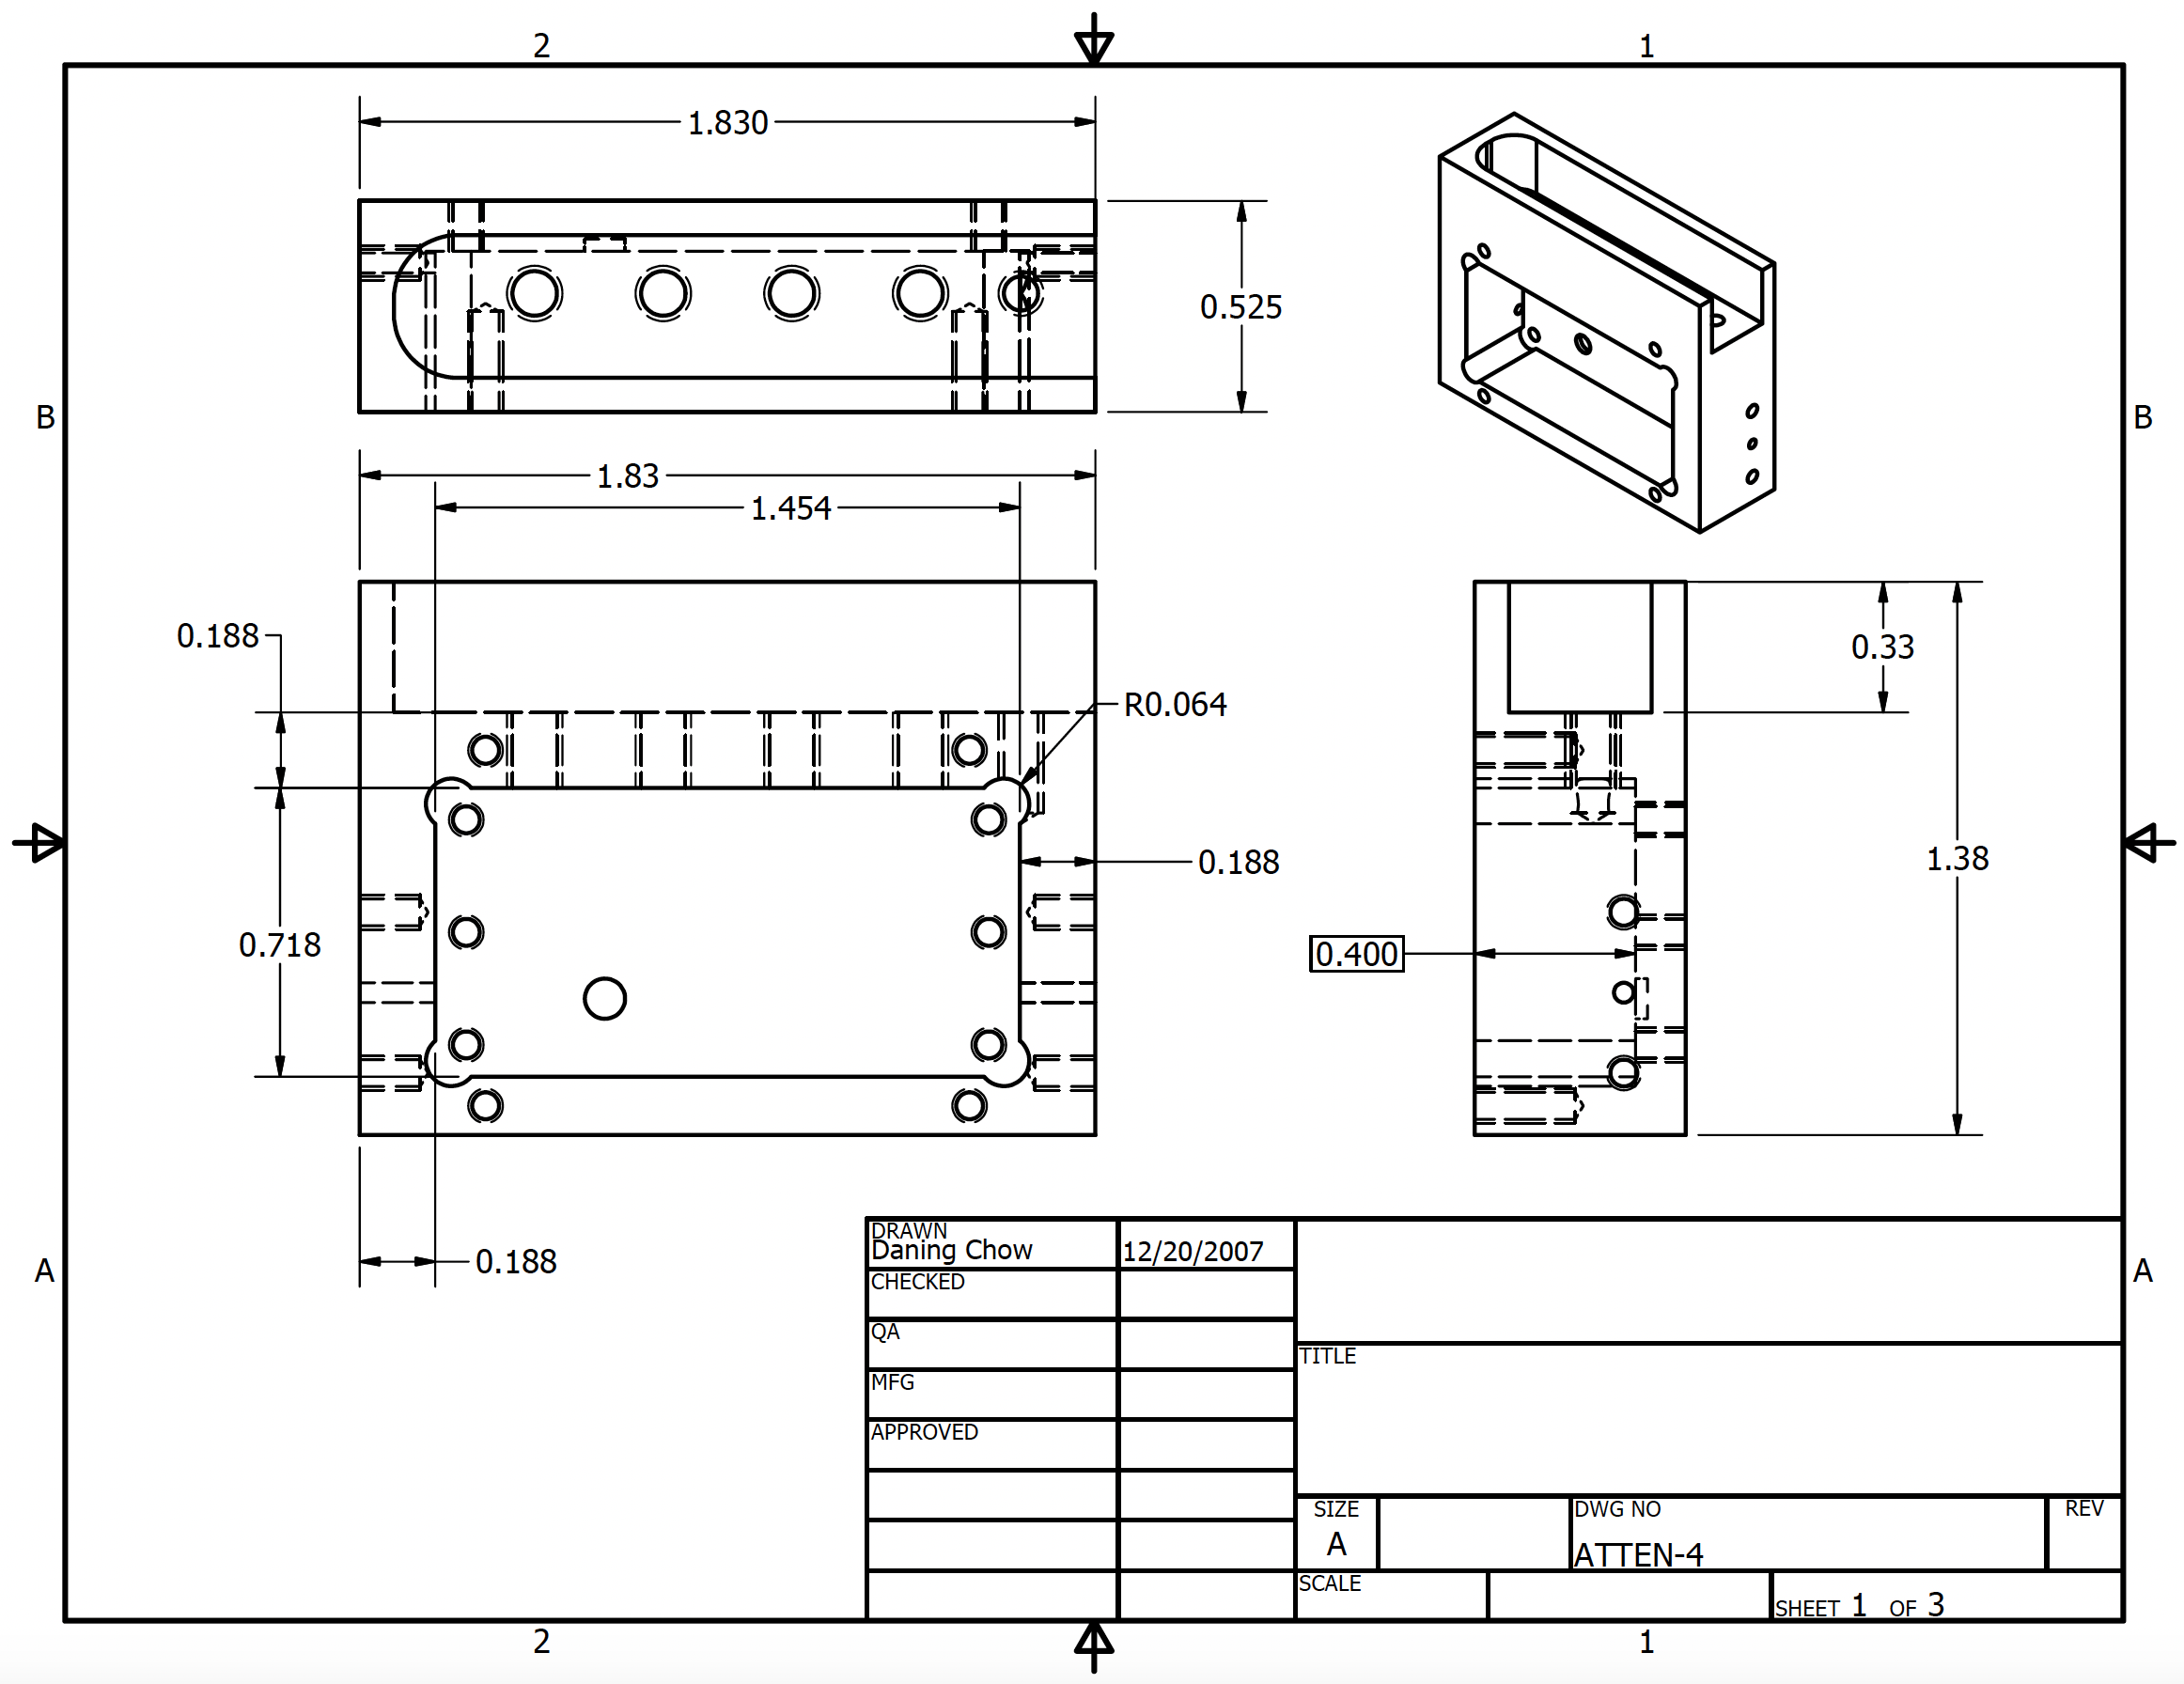
\includegraphics[width=.6\linewidth]{Documentation/figures/Attemp_Enc1.png}
 \caption{1050-A Attemplifier Enclosure Drawing 1}
 \label{fig:Attemp_Enc1}
 \end{figure}
 
 \begin{figure}[H]
 \centering
 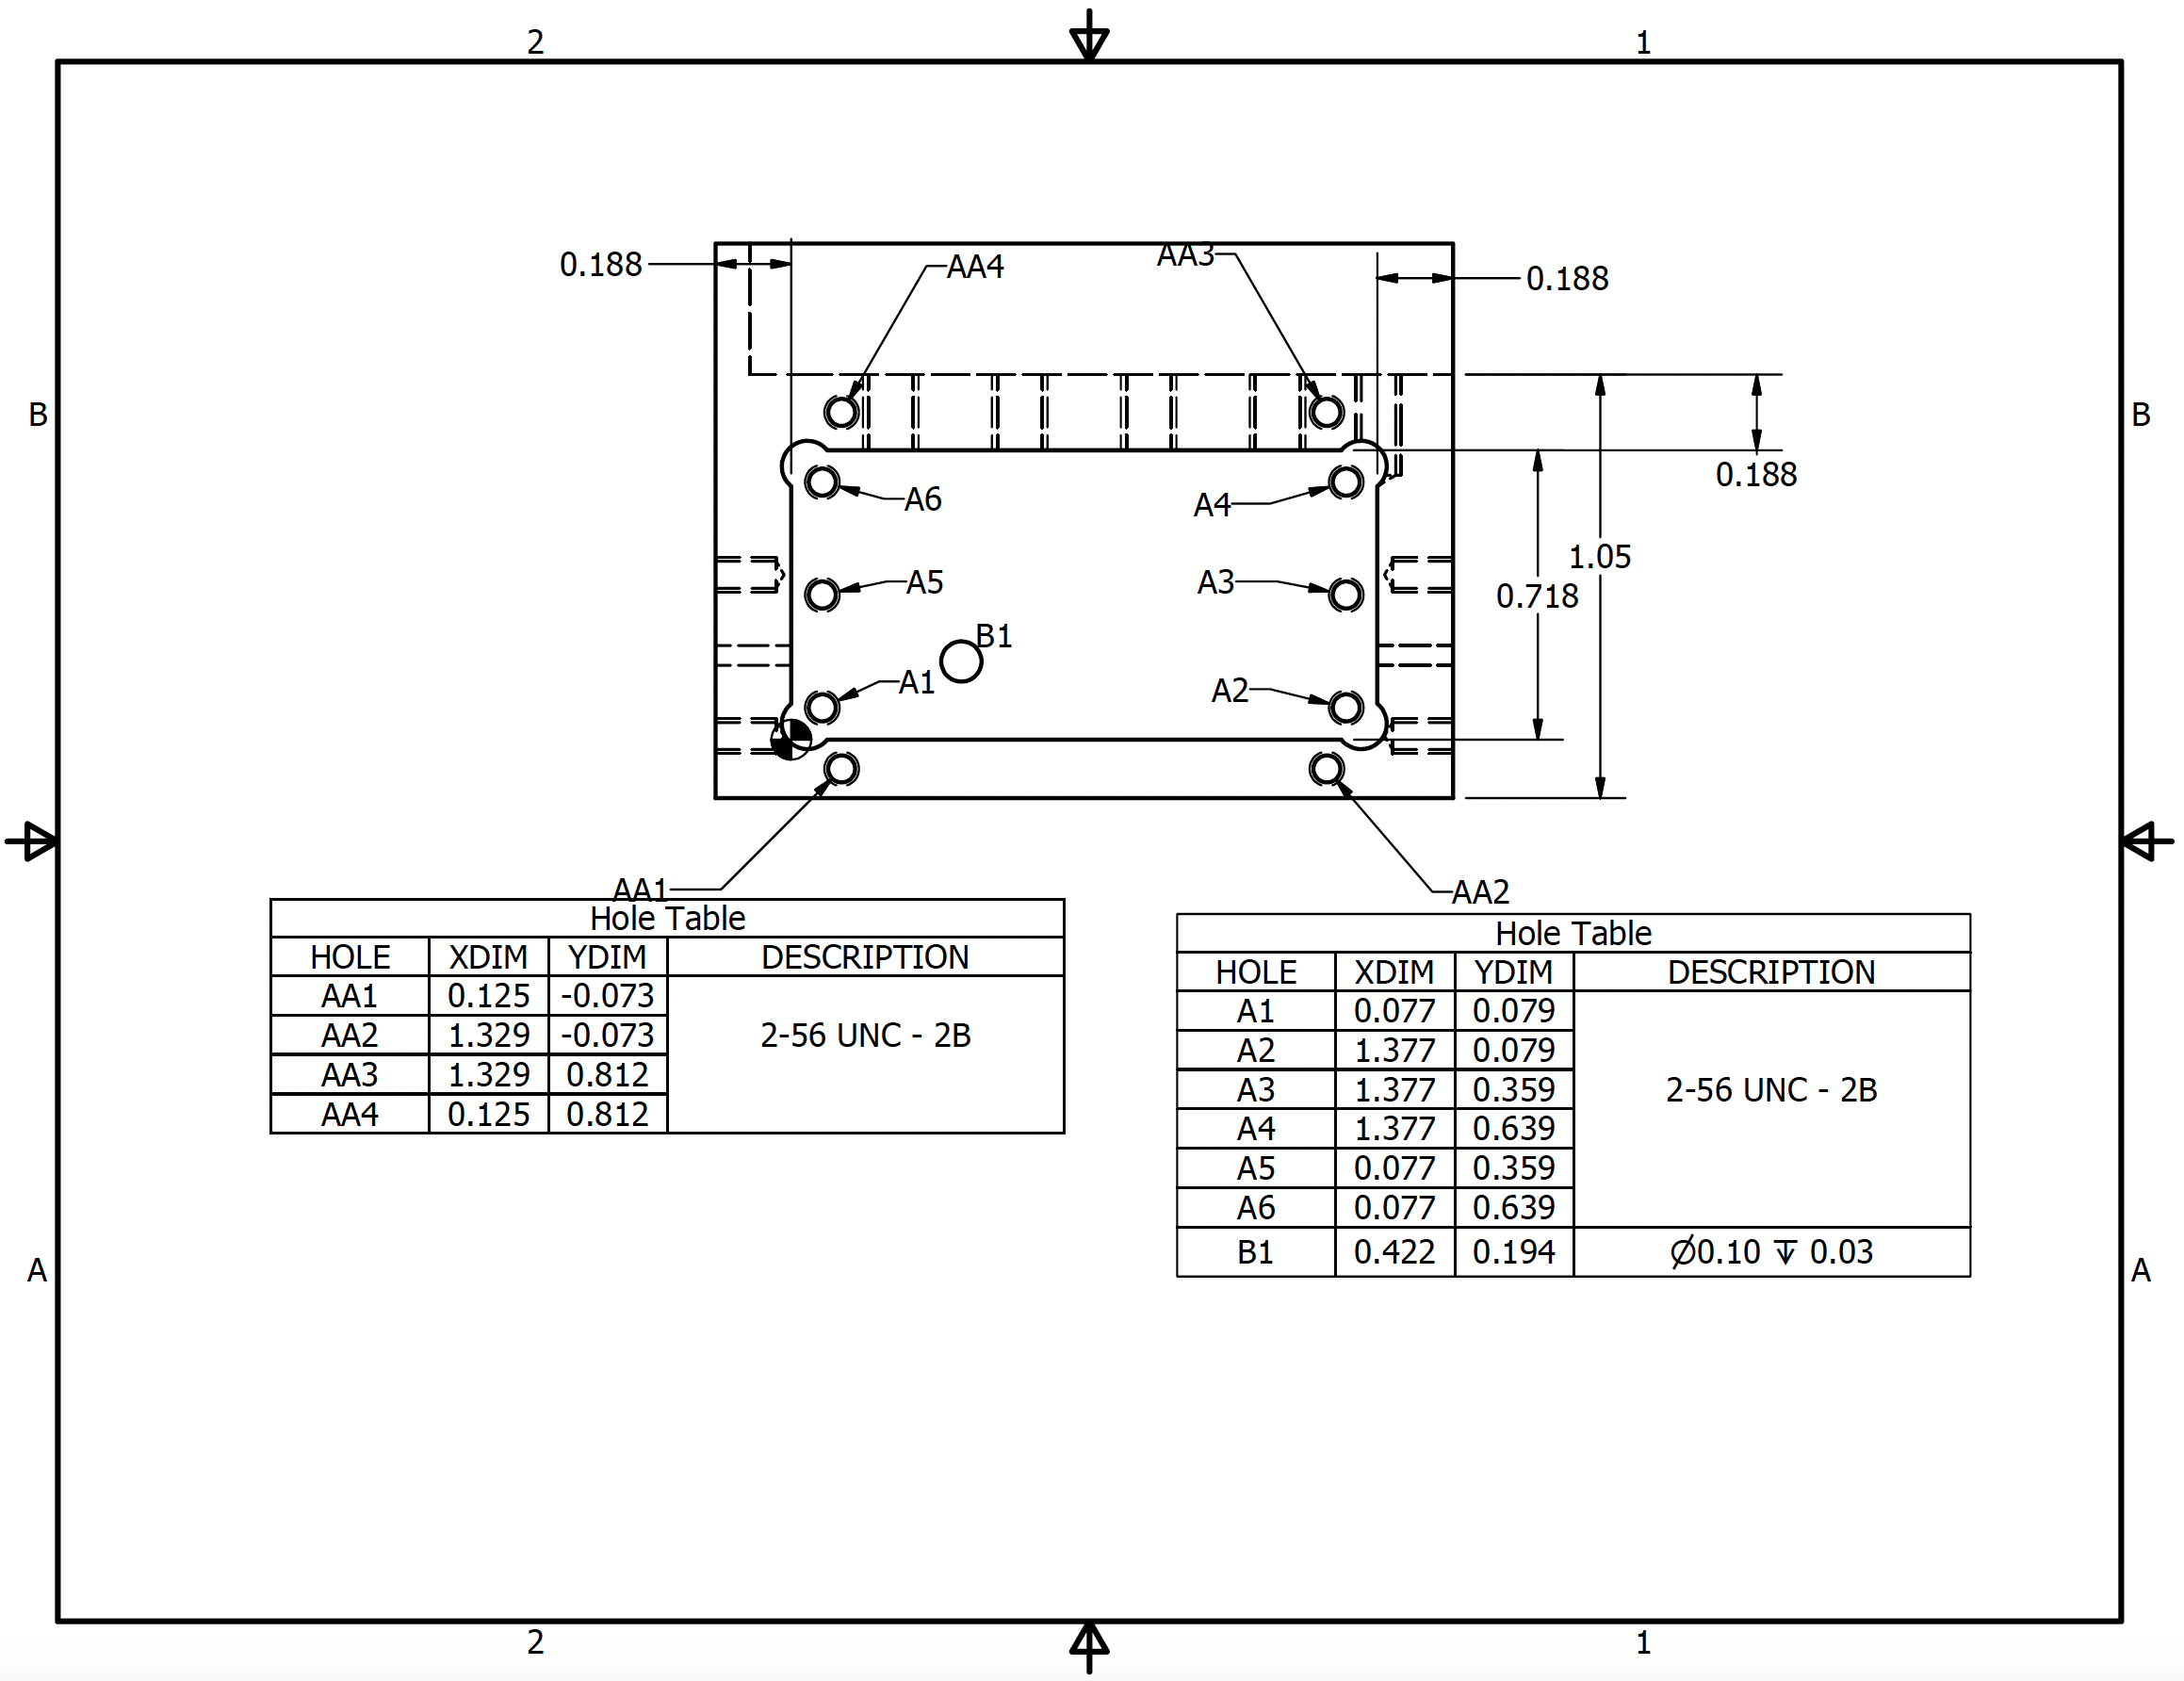
\includegraphics[width=.8\linewidth]{Documentation/figures/Attemp_Enc2.png}
 \caption{1050-A Attemplifier Enclosure Drawing 2}
 \label{fig:Attemp_Enc2}
 \end{figure}
 
 
 \begin{figure}[H]
 \centering
 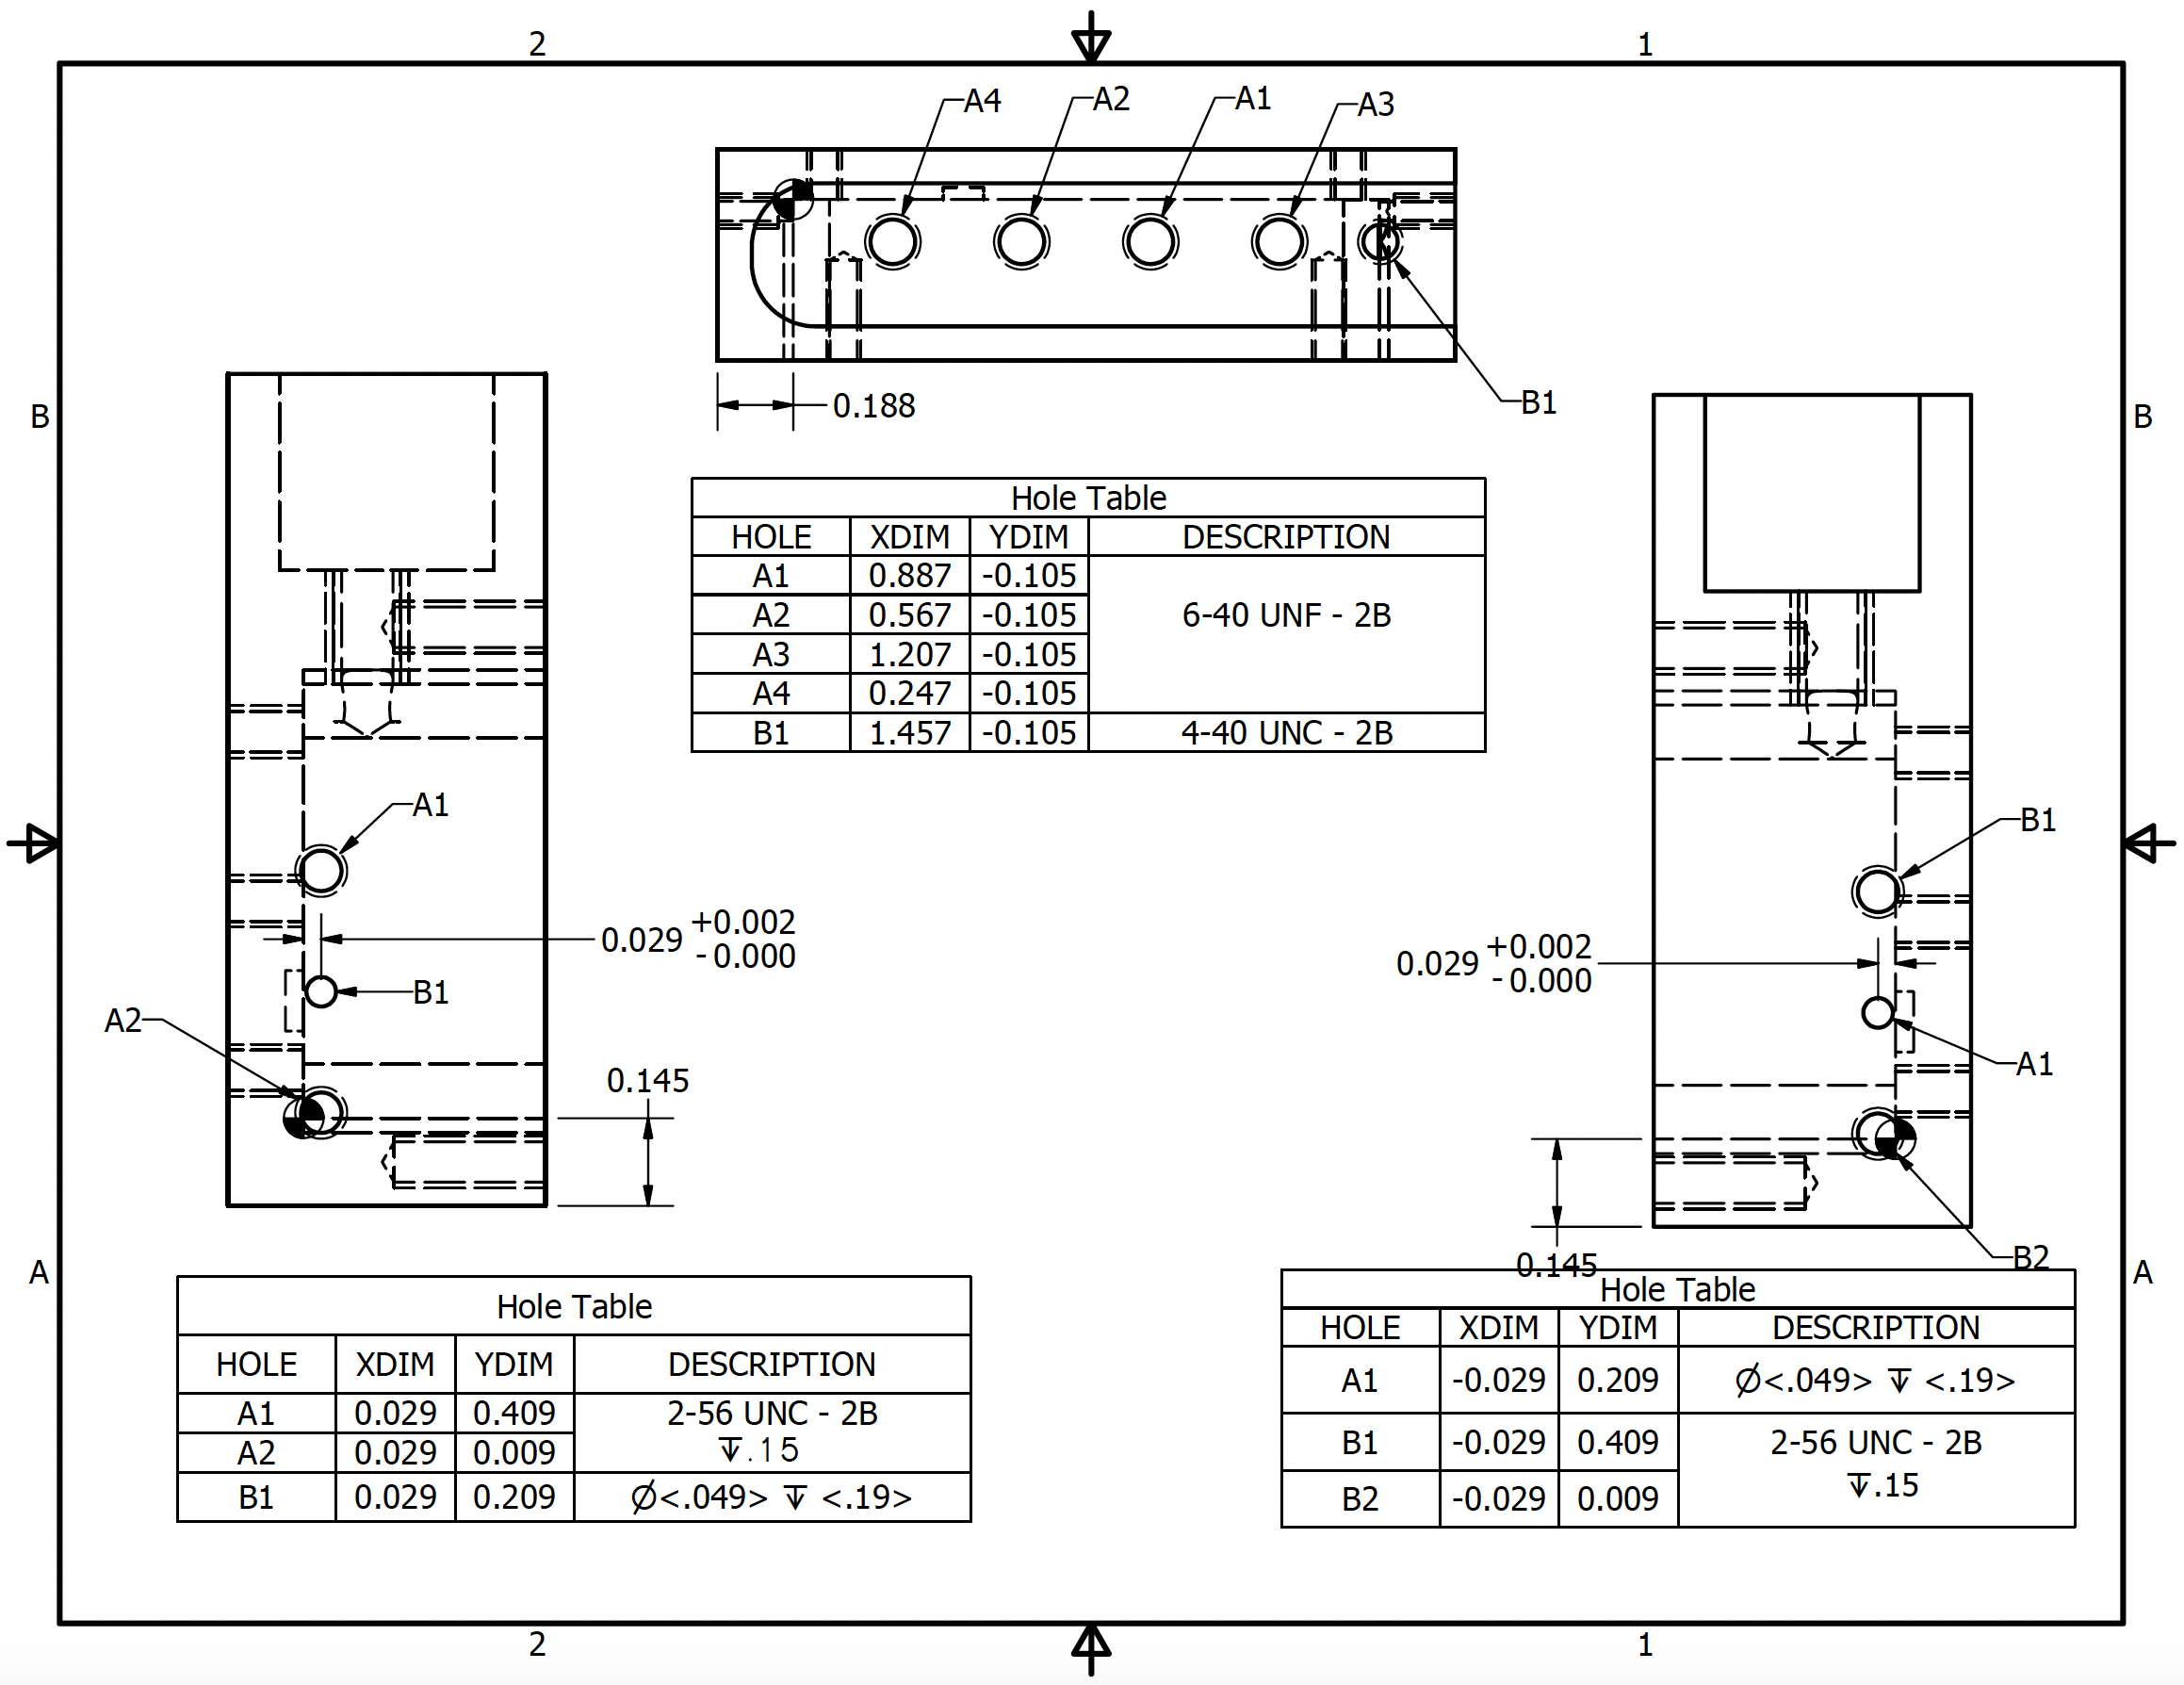
\includegraphics[width=.8\linewidth]{Documentation/figures/Attemp_Enc3.png}
 \caption{1050-A Attemplifier Enclosure Drawing 3}
 \label{fig:Attemp_Enc3}
 \end{figure}

\end{landscape}

\end{document}
